%\setcounter{chapter}{7}
\chapter{Module Production for the Phase I CMS Pixel Detector Upgrade}\label{ch:phase1}

As discussed in chapter \ref{ch:lhcandcms}, radiation has a big impact on the CMS pixel detector causing damage to its components throughout its lifetime, therefore this detector needs to be periodically upgraded. The first version of the detector was known as phase 0, it was installed in 2008 and became fully operational in 2010 after a magnet failure caused a delay in the LHC original starting date. In 2017 the pixel detector was replaced during the phase I pixel upgrade. From 2013 to 2106 the University of Nebraska, high energy group (UNL-HEP) played a major role in assembling and testing, which then became part of the forward region of the pixel detector. The next generation of the pixel detector, the phase II upgrade, is projected to take place in 2025 when the current detector will be reaching its radiation limits and its performance will be deteriorated. In this chapter we describe why the phase 0 pixel detector needed an upgrade and the main changes done to it. We also present a description of the module assembly and testing process at UNL. Some of the steps in the process will be highlighted and in detailed as they were my contributions to the production campaign.

%Special attention is making and {\rojo{describe}} the work done by the UNL-HEP group.  %Specially the  and highlighting 

\section{The CMS Forward Pixel Detector Phase I Upgrade}
{\rojo{how many modules}} 768 or 672.\\ 
%The CMS pixel detector is composed of two sections, the barrel section (BPix) and the forward section (FPix). Each of these sections (for phase 0) was composed of three layers originally designed to record three 3D positions (tracks) of the particles emerging from the \ital{pp} collisions. As well as to provide information to reconstruct primary and secondary vertices of decaying particles. 
The phase 0 detector performed well during the LHC run I, taking data at a peak luminosity close to $7$ x $10^{33} cm^{-2} s^{-1}$ and energy of 8 TeV. This data was used in many physics analysis including the discovery of the Higgs bosson published in 2013. But after a few years of operation the pixel detector started to degrade due to radiation damage, causing an increase of fake rates as well as loose on resolution. Moreover, for run II the LHC physics program planned three major updates: to more than double its luminosity with successive increment until it reaches its peak of $2$ x $10^{35} cm^{-2} s^{-1}$, to increase the center of mass energy to 13 TeV and finally to its design value of 14 TeV, reduce the bunch crossing from 50 ns to 25 ns hence increasing the amount of pile up per interaction. As it was designed the phase 0 pixel detector could not withstand such collision conditions. Therefore plans began to design and construct a new and improved detector that could perform effectively in the new LHC running conditions. Figure \ref{redperf} shows a comparison in performance of the previous (top) and the current (bottom) pixel detector under different luminosity  and pile-up conditions. %It is evident 
%A simulation of the performance of the pixel detector under different luminosity conditions can be seen in figure \ref{fig:red_perf}. 

\begin{figure}[!h]
	\centering
	\includegraphics[width=0.6\textwidth]{ch7/reducedperformance}
	\includegraphics[width=0.6\textwidth]{ch7/reducedperformance}
	\caption[Simulated performance comparison of previous and current]{Simulated performace of the previous pixel detector (top) and current (bottom) under different conditions using a $t\bar{t}$ sample: a) track-finding efficiency; b) fake rate. Conventions are the same for both plots, considering zero pileup (blue squares), average pileup of 25 (red dots), average pileup of 50 (black diamonds), and average pileup of 100 (magenta triangles) {\rojo{find figure}}.\cite{pix_tdr}.}
	\label{redperf}
\end{figure}

%Figure \ref{pixeloldandnew} compares the old and the new pixel detector 


For the current pixel detector a new layer was added to the barrel and the forward region, as shown in figure \ref{pixeloldandnew}. The three FPix endcap disks are located at 29.1 cm, 39.6 cm, and 51.6 cm from the interaction point. Compared to the old FPix, the innermost disk is 4.4 cm closer to the interaction point. This provides a four-hit coverage for tracks ranging up to $\pm$ 2.5 in pseudorapidity. To reduce the extra material added by the extra layer of the pixel detector a lightweight support was used, a CO2 cooling system was adopted, and inactive materials were moved away from the tracking area. % To avoid the increase of material that an additional layer signifies, several step by the addition of the extra layer
Figure \ref{pixelmaterial} shows the amount of material needed for both the old and the current pixel detector as a function of eta.


\begin{figure}[!h]
	\centering
	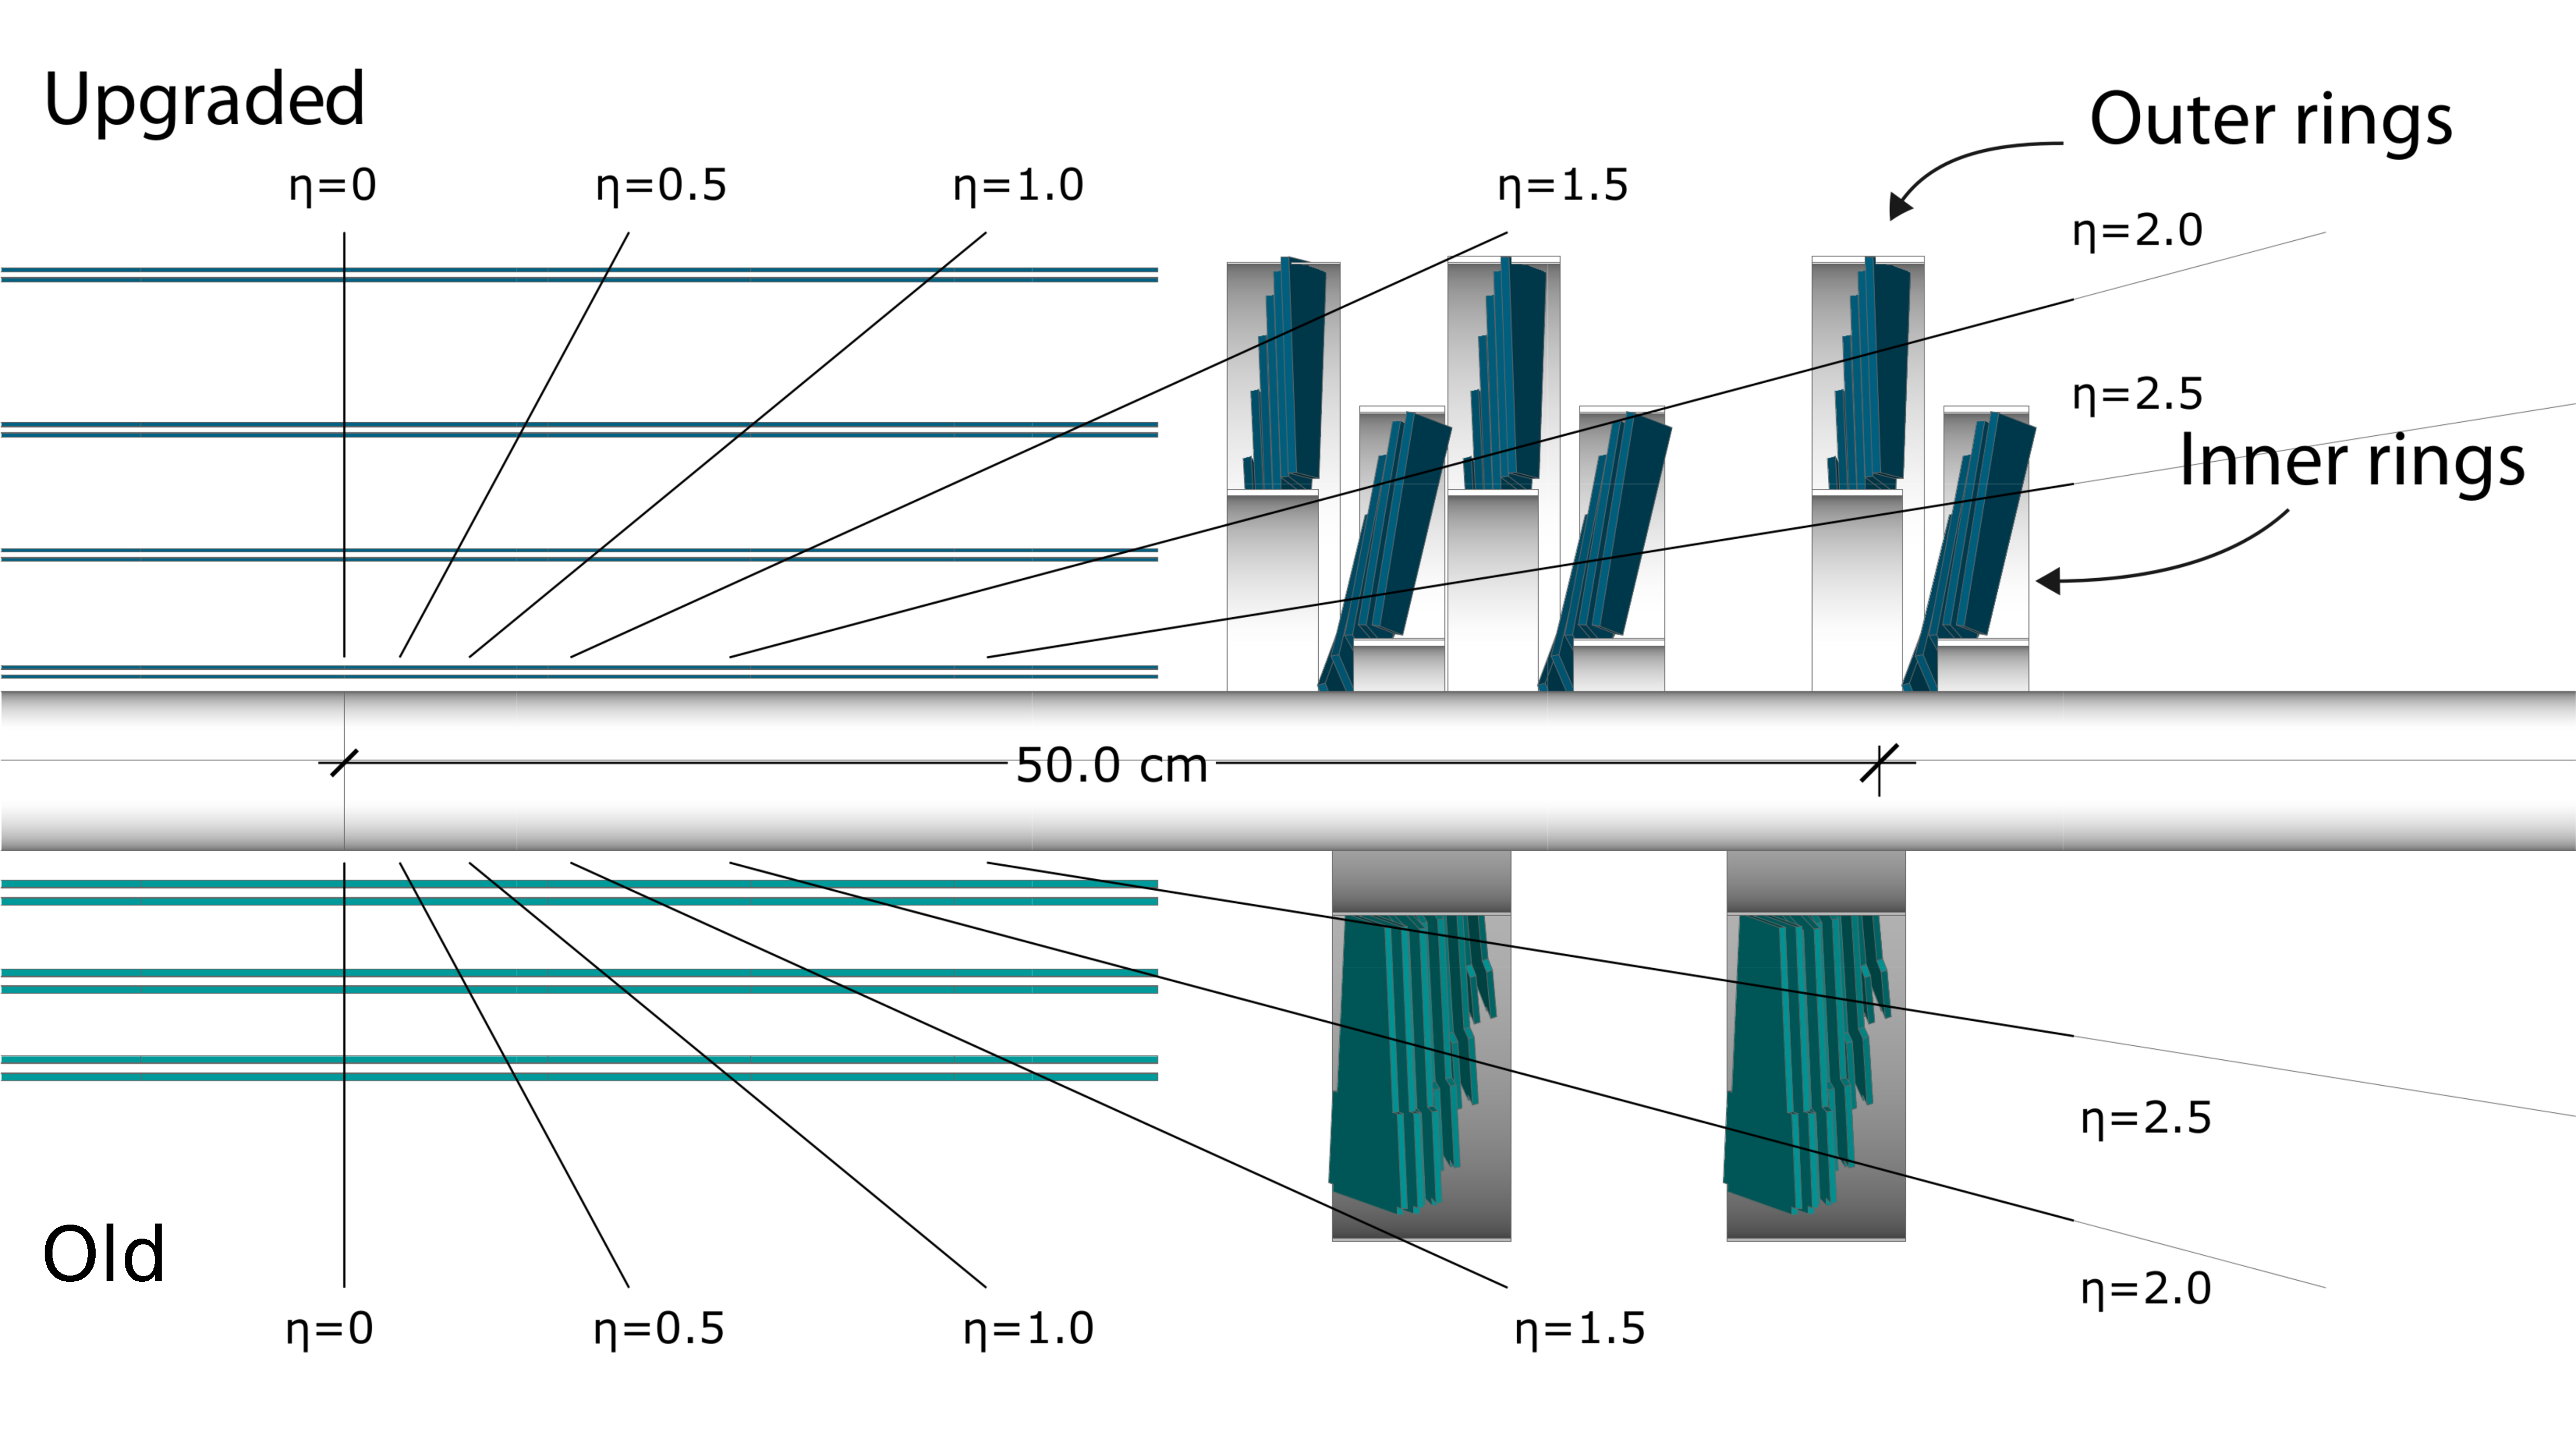
\includegraphics[width=0.6\textwidth]{../images/ch7/fpix.pdf}
	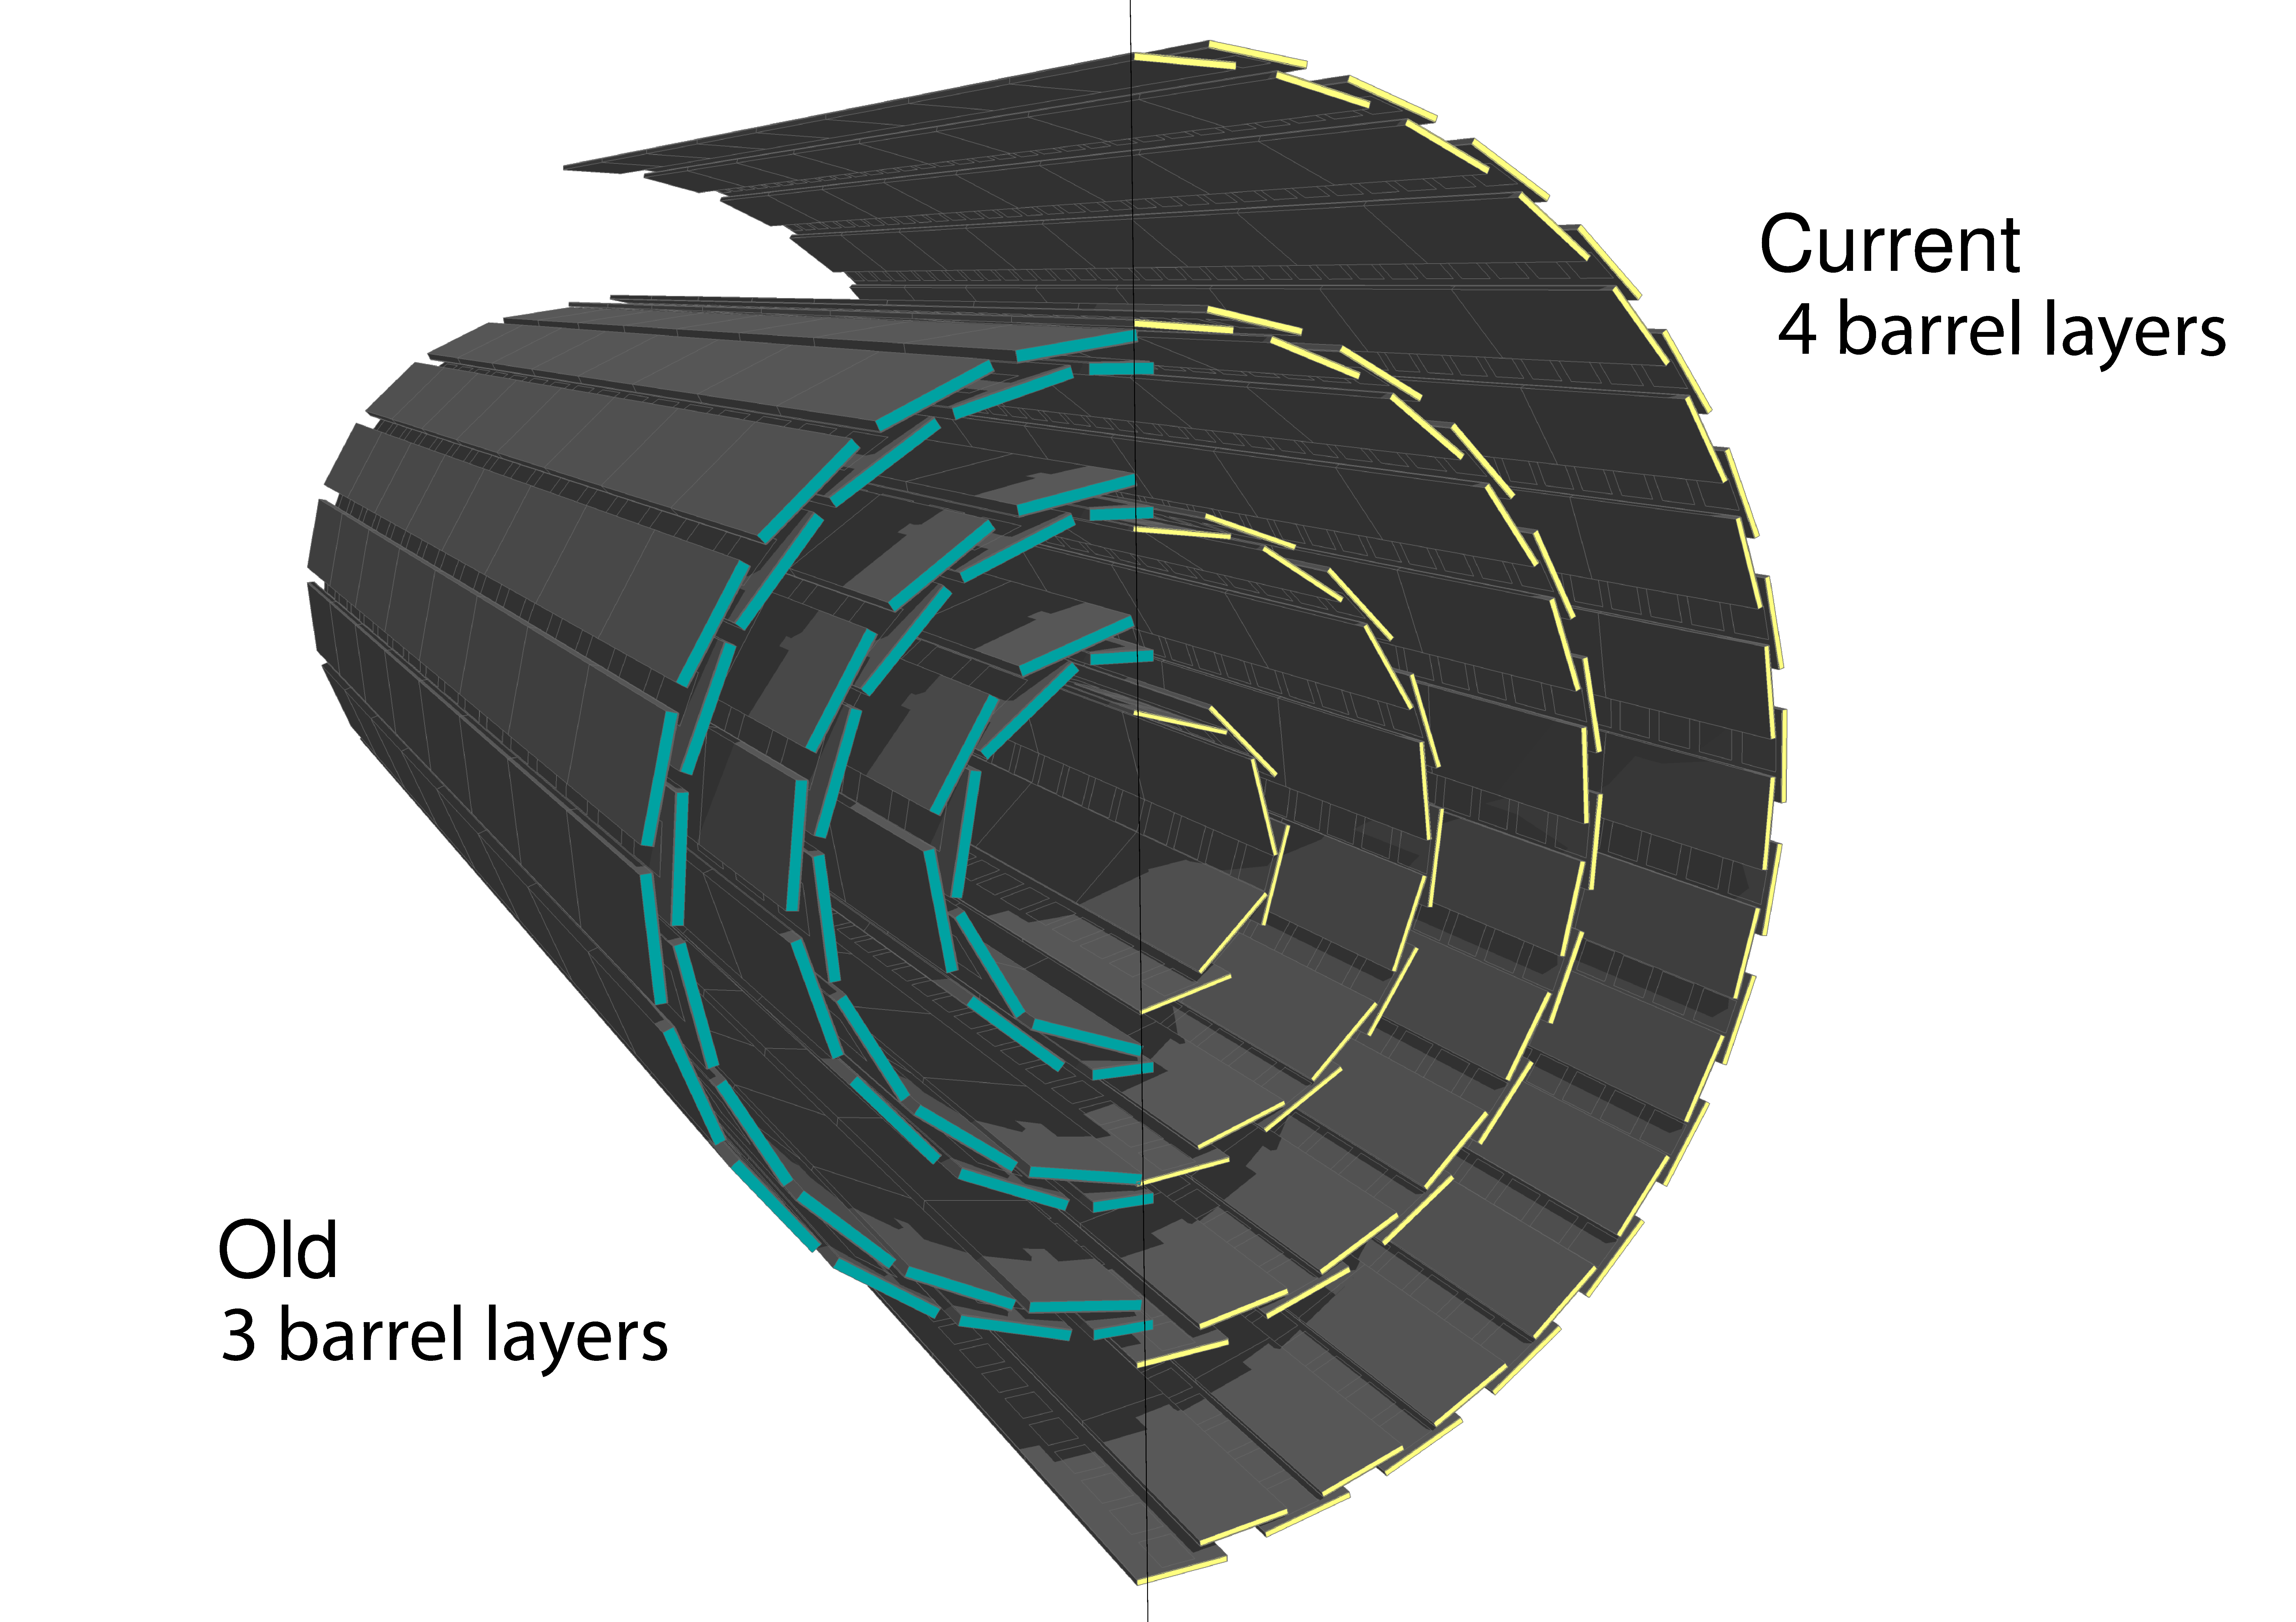
\includegraphics[width=0.39\textwidth]{../images/ch7/bpix.pdf}
	\caption[Layout of the upgraded and old pixel detectors.]{Layout and comparison of the layers and disks in the upgraded (Phase I) and old (Phase 0) pixel detectors \cite{pix_tdr}.}
	\label{pixeloldandnew}
\end{figure}

%\begin{figure}[!h]
%	\centering
%	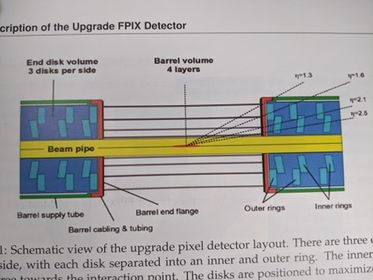
\includegraphics[width=0.9\textwidth]{ch7/schematic_pixel_det}
%	%\includegraphics[width=0.9\textwidth]{pixel/reducedperformance}
%	\caption[Schematic view of the pixel detector]{Schematic view of the pixel detector highlighing the positions of the disks to maximize the 4 hit eta coverage \cite{pix_tdr}.}
%	\label{schematicofpixeldetector}
%\end{figure}



%\begin{figure}[!h]
%	\centering
%	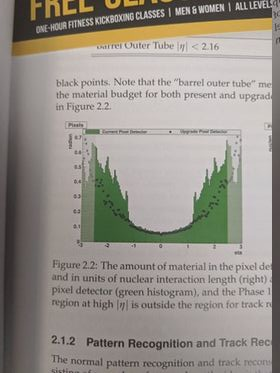
\includegraphics[width=0.9\textwidth]{ch7/pixel_material}
%	\caption[Material used by the pixel detector]{Material used by the old (green histograms) and current (black dots) pixel detector \cite{pix_tdr}.}
%	\label{pixelmaterial}
%\end{figure}

In general the geometry of the current FPix is similar to the old detector. The three disks are vertically divided into half-disks, and are composed of inner and outer disks. This allows for easy assembly and disassembly for repairs when necessary. Each of these three disks are mounted on half cylinders, which also contains the CO2 cooling tubes and the readout electronics as shown in figure \ref{halfdisk}. Each half disk contains 56 modules bringing the total number of modules for the FPix to 672. One key difference between the old and current detector is the use of one single module type in a 2x8 array. This made easier the installation compared to the old detector.   

\begin{figure}[!h]
	\centering
	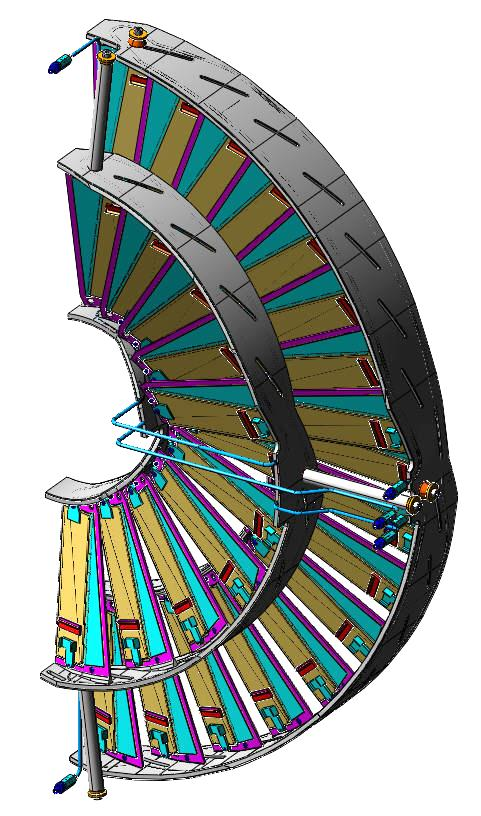
\includegraphics[width=0.2\textwidth]{ch7/half_disk}
	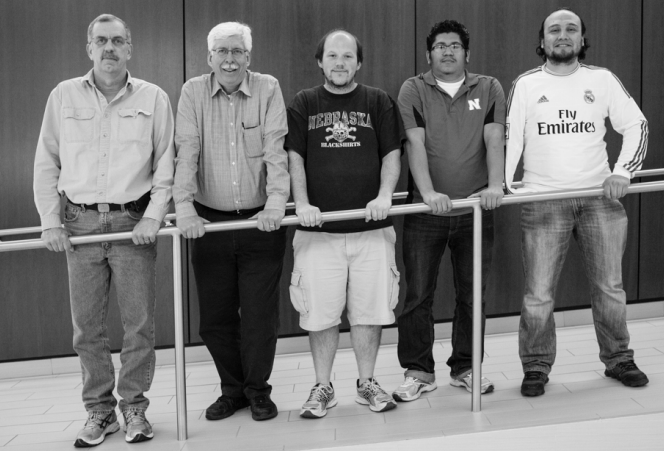
\includegraphics[width=0.2\textwidth]{ch7/aaaa}
	\caption[Half disks and half cylinder]{Half disks and half cylinder for the forward pixel detector \cite{pix_tdr}.}
	\label{halfdisk}
\end{figure}
Modules are composed of 16 read out chips (ROCs) and each ROC is form by 4160 pixels of 100mm x 150 mm. {\rojo{improve of module and readout}}
Modules are mounted on the inner and outer half disks and not attached to the half cylinder. This allows damaged modules to be replaced without having to disassembly the half cylinder. The modules in the inner ring are rotated by 12 degrees towards the interaction point to improve resolution in both the azimuthal and radial direction.

\section{Module Production at UNL}
The module production for the FPix was a join effort among several US institutions. University of Nebraska and Purdue University were assembly sites, Kansas University was x-ray testing site, and modules were finally tested and incorporated to the disks in the silicon laboratory detector at FermiLab.

The assembly process workflow at UNL was designed to follow a pipeline-like structure as shown in figure \ref{fig:unlworkflow}. This allows for different batches of modules to be going through it at different stages without stopping the workflow. Following is a short description of the tests and procedures performed during the production in the UNL silicon Lab. Special emphasis will be made in IV test, visual inspection and electrical test, the stages where the author of this work made a lot of contributions {\rojo{improve}}. 

%{\rojo{mention 4 sites}}

\begin{figure}[!h]
	\centering
	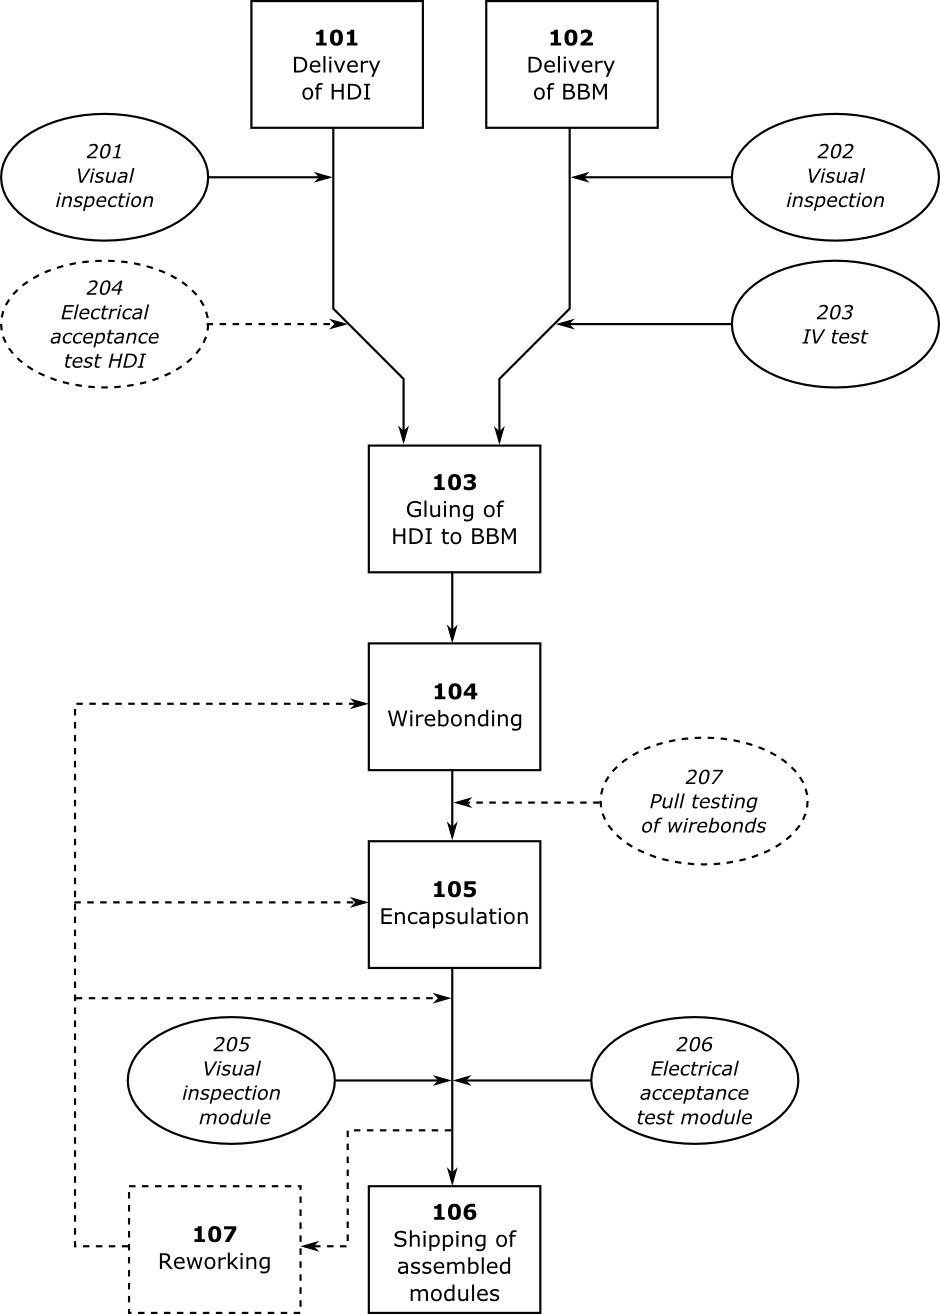
\includegraphics[width=0.7\textwidth]{../images/ch7/unl_workflow}
	\caption[UNL module assembly workflow]{UNL module assembly workflow. Dashed lines represent occasional quality testing and reworking procedures\cite{ph1_sop}.}
	\label{fig:unlworkflow}
\end{figure}

\subsection{Visual Inspections}
The UNL-HEP group assembly workflow started upon receiving two components: a Bare Bonded Module (BBM) and a High Density Interconnect (HDI), see figure \ref{fig:bbmyhdi}. The first stage of the module production was a visual inspection on these components to ensure they were in good conditions and able to continue into the production pipeline.

\begin{figure}[!h]
	\centering
	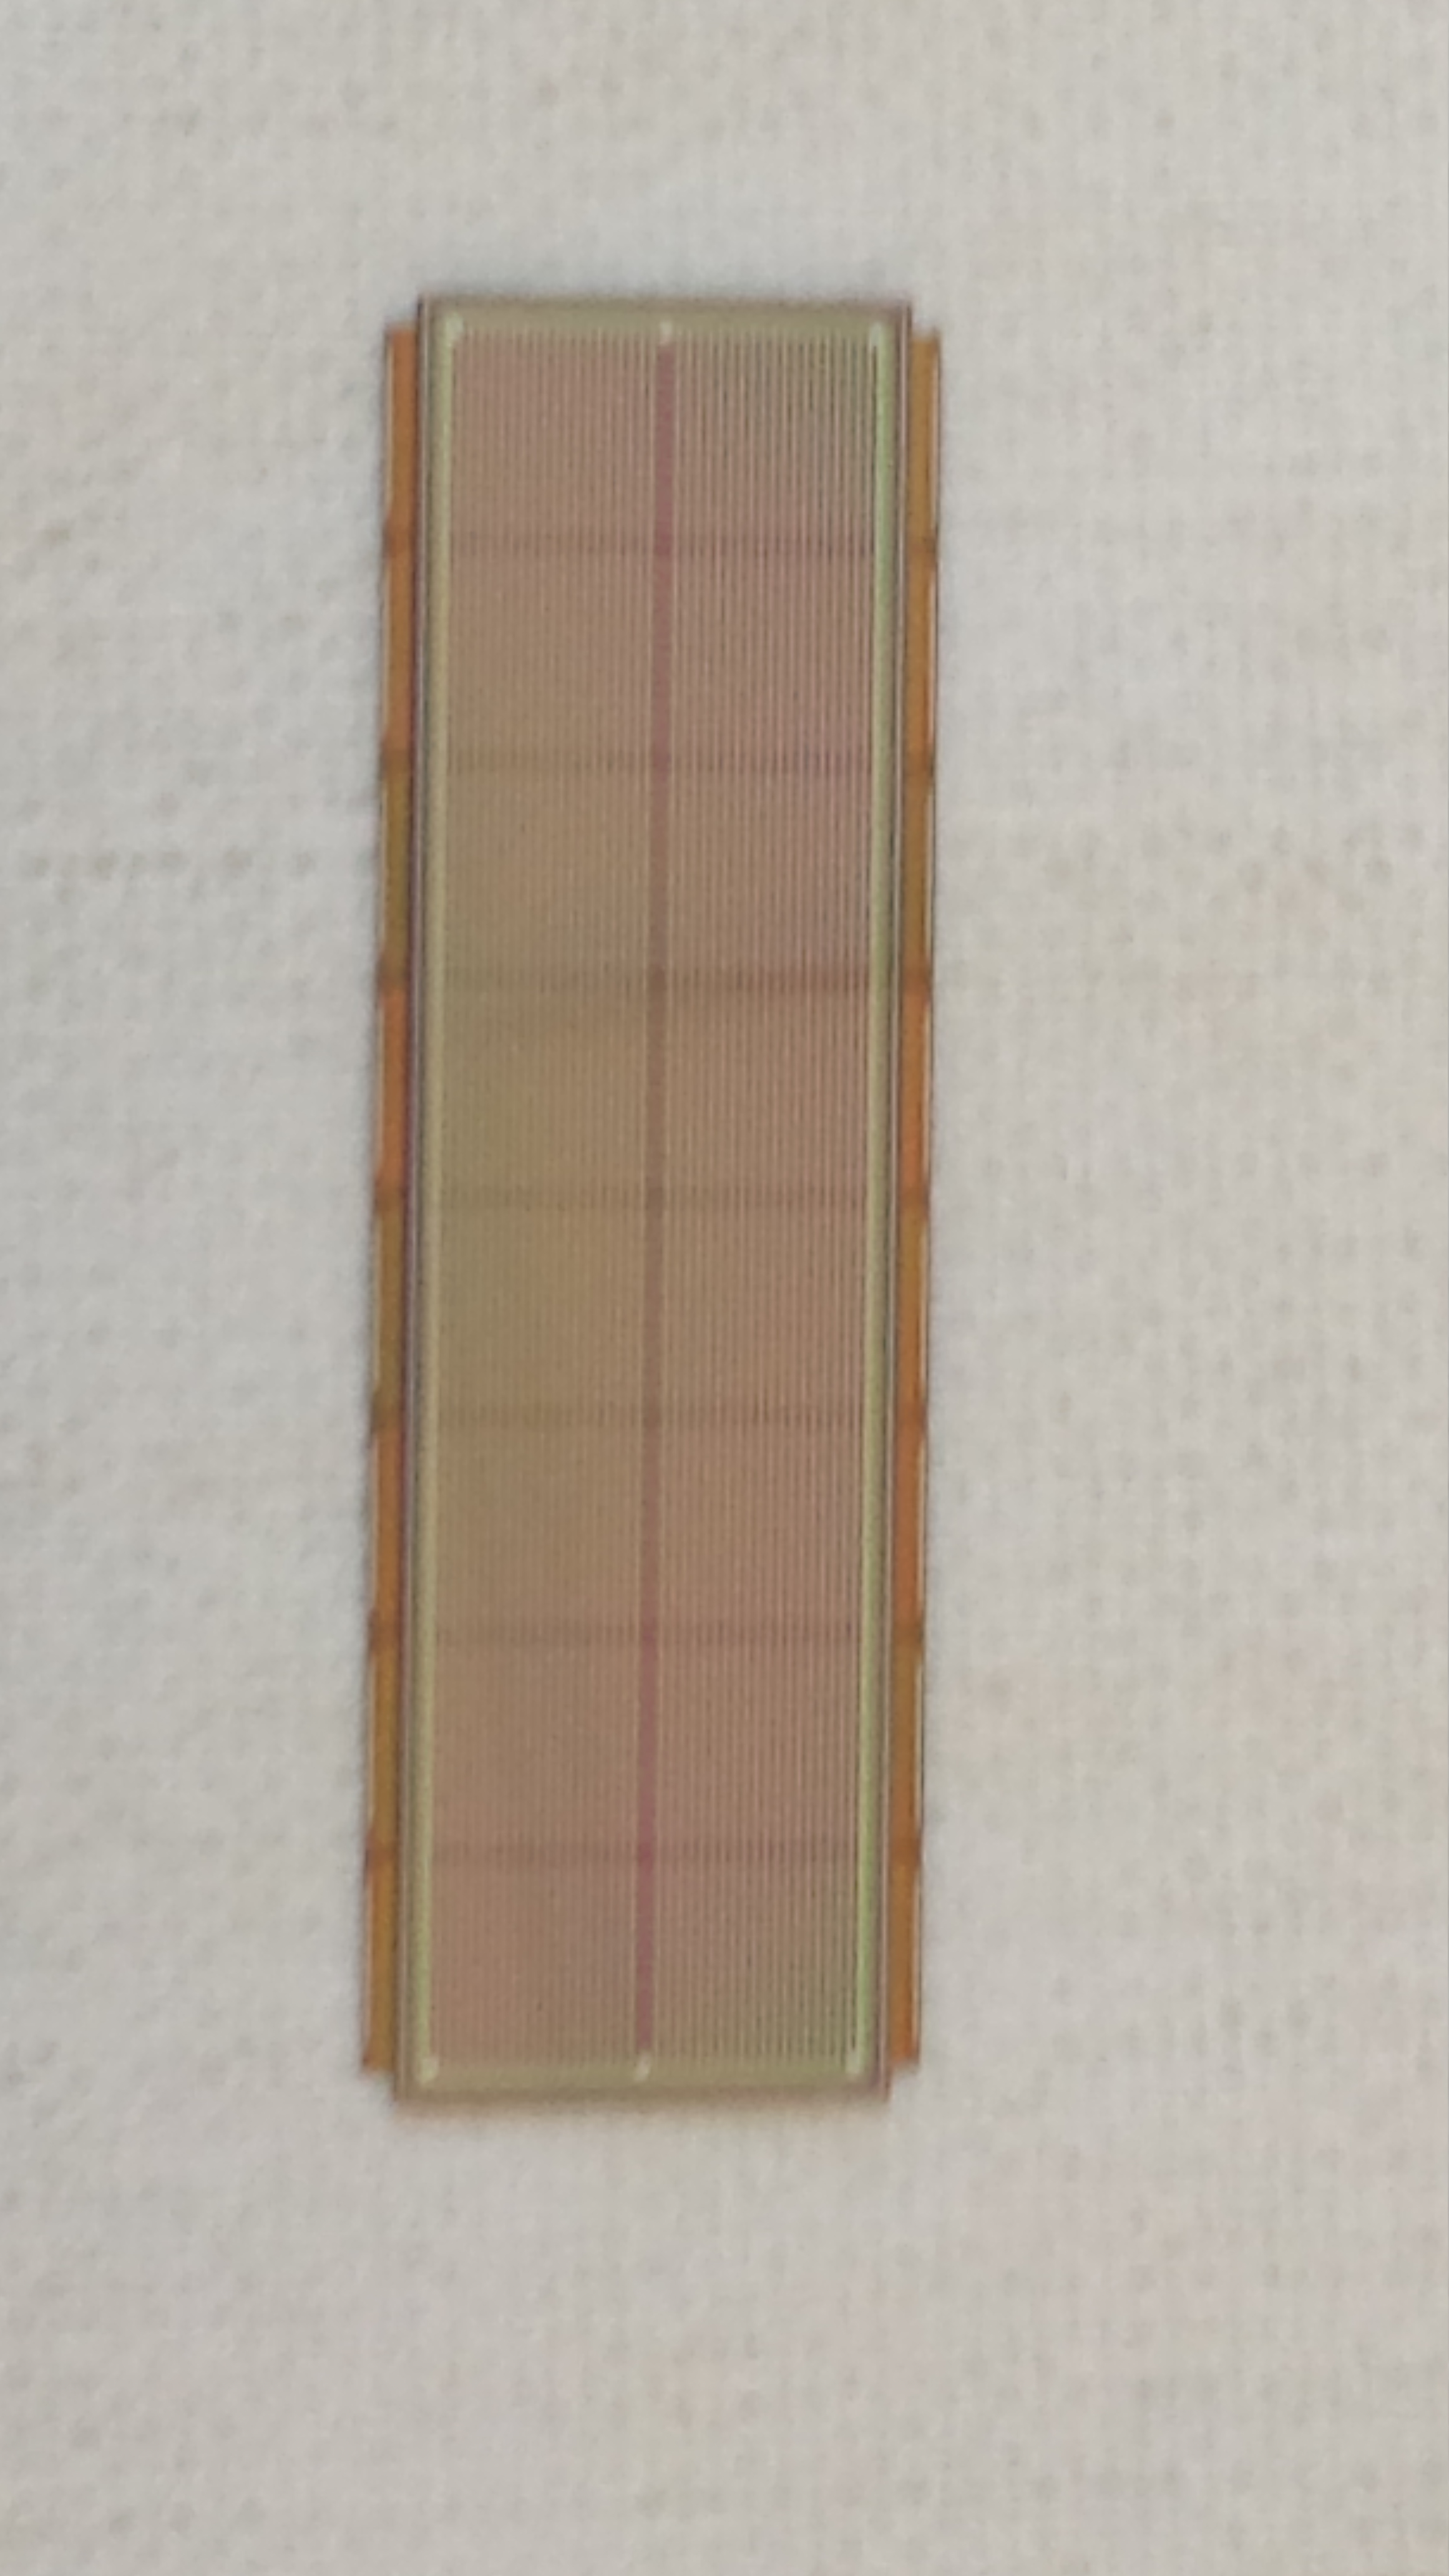
\includegraphics[width=0.3\textwidth]{ch7/bbm}
	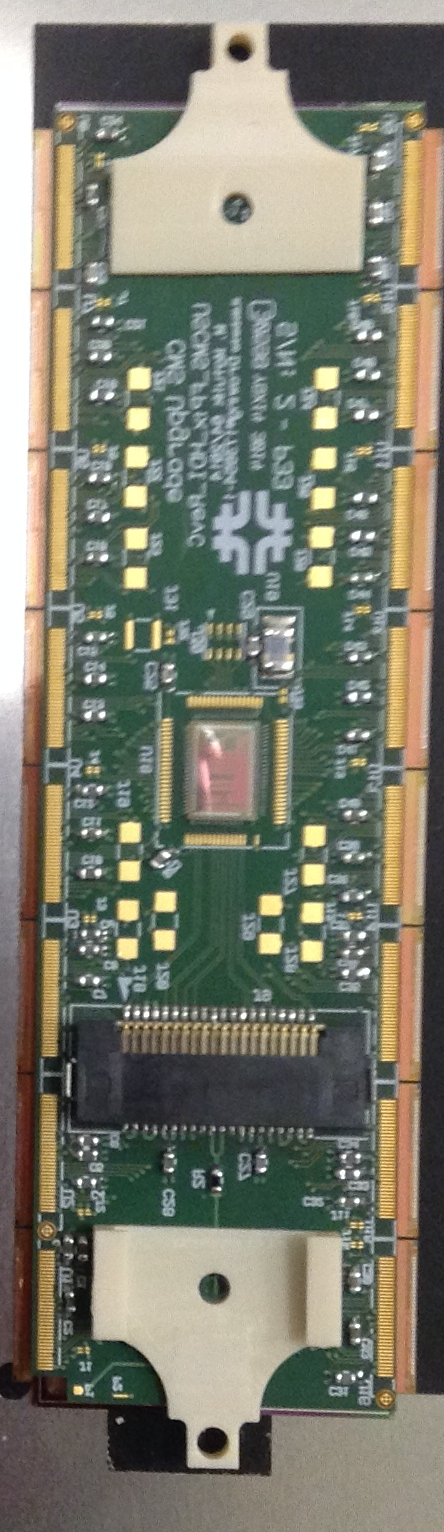
\includegraphics[width=0.3\textwidth]{ch7/hdi}
	\caption[Photograph of a BBM and HDI.]{Photograph of a BBM (left) and HDI (right) as received by the UNL-HEP group.}
	\label{fig:bbmyhdi}
\end{figure}

To get a good view of such a small components a powerful microscope with magnification of {\rojo{confirm}}, an attached camera, and LED ring illumination was used. A photograph of the set up, also referred to as probe station, is shown in figure \ref{fig:probe_station}. The entire set up was connected to a vacuum line to secure these component in place and avoid any damage during the visual inspection. BBMs were received in a gel pack while HDIs were usually received in their modules carriers. BBMs and HDIs were then moved into the probe station using a vacuum pen and taking the appropriate safety precaution: ESD wristband, gloves, face mask, etc.

\begin{figure}[!h]
	\centering
	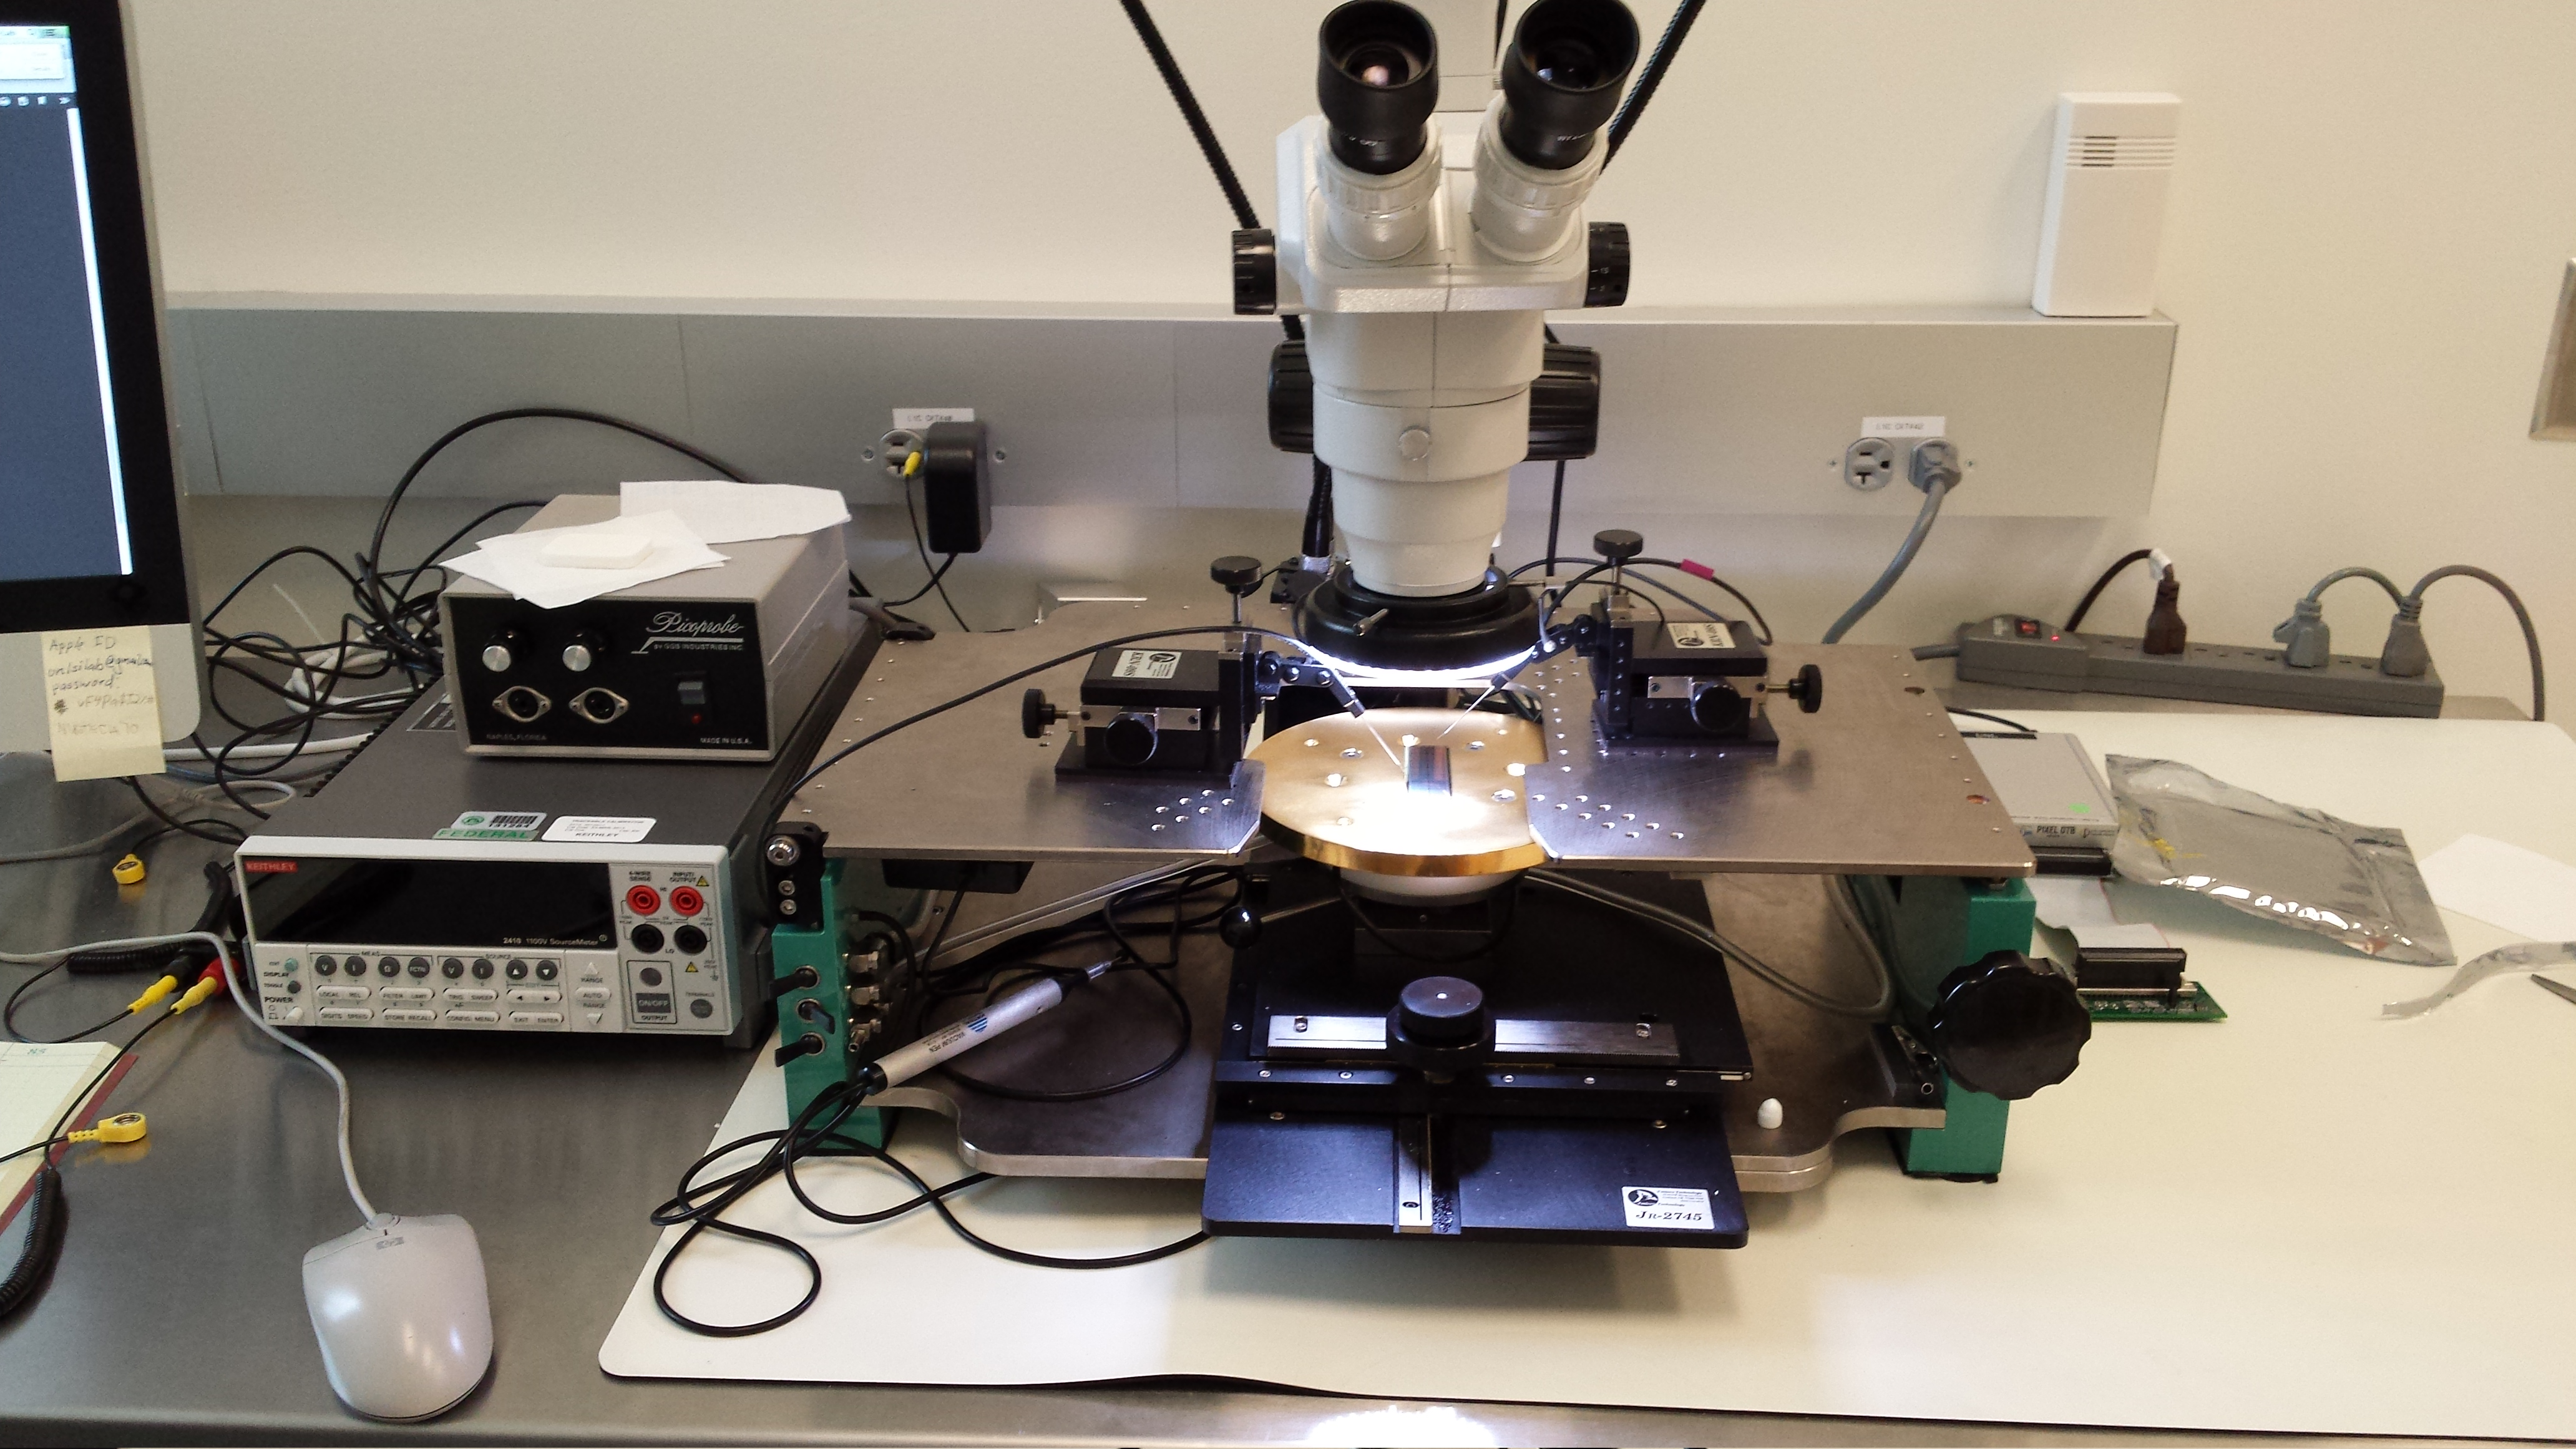
\includegraphics[width=0.7\textwidth]{ch7/probe_station}
	\caption[Photograph of the visual inspection and IV test station.]{Photograph showing a BBM under the microscope during a visual inspection. This station also served as IV test stand.}
	\label{fig:probe_station}
\end{figure}

During visual inspection BBMs were scanned for unusual features or sign of damage, special attention was given to the high voltage connection and bond pads. Figure \ref{fig:vis_insp_bbm} shows different parts of four different modules where defects on three of them could be observed. Some of these defects, bottom right figure, caused the module to be rejected immediately while others, bottom figures, will still undergo an IV test. While for the HDI the bond pads of the 16 ROCs, the wirebonds of the tbm, and the address pads were carefully checked. Figure \ref{fig:vis_insp_hdi} shows the TBM wirebonds as well as the bondpads of a ROC in a HDI.

\begin{figure}[!h]
	\centering
	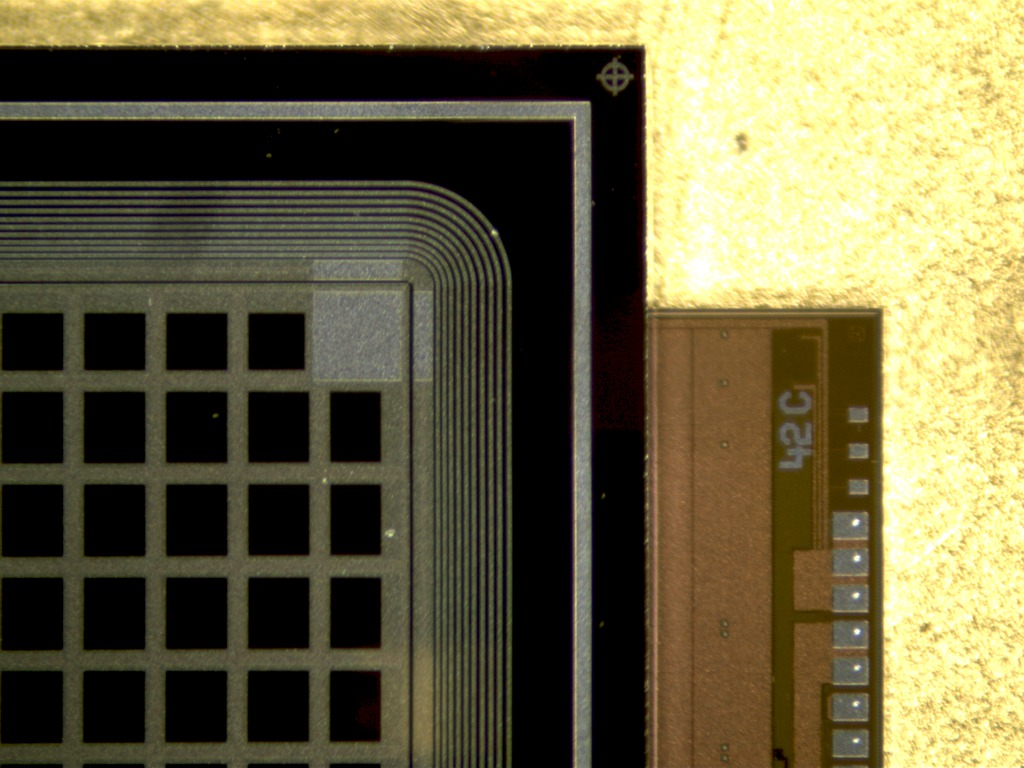
\includegraphics[width=0.4\textwidth]{ch7/vis_insp_1}
	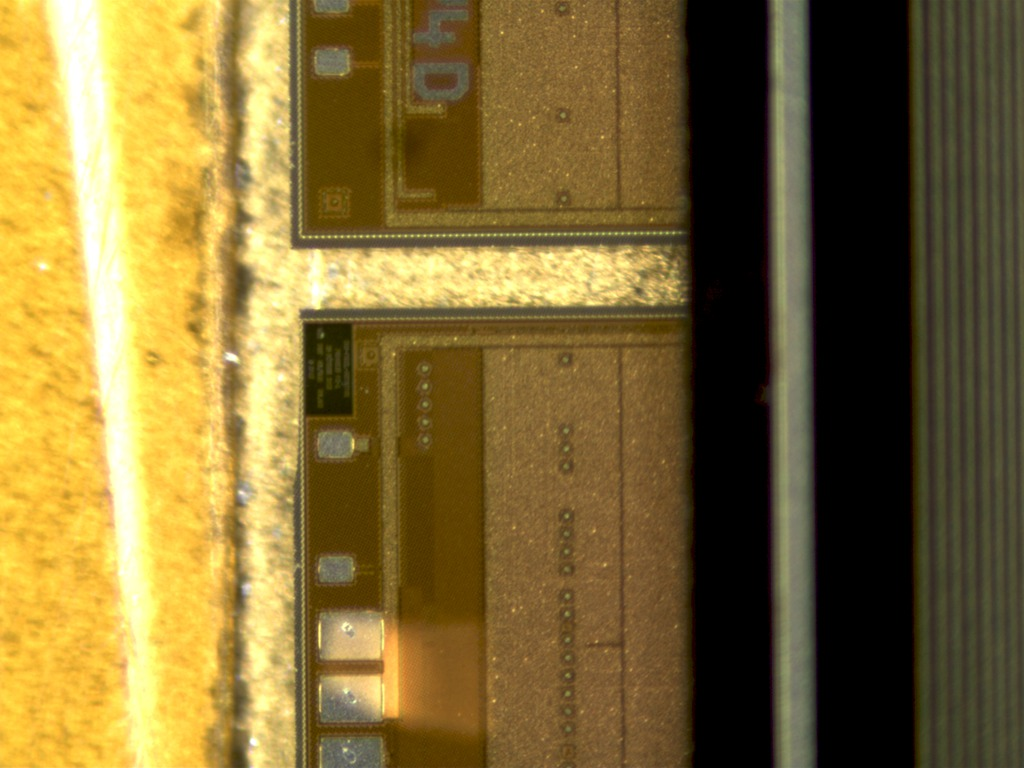
\includegraphics[width=0.4\textwidth]{ch7/vis_insp_5}
	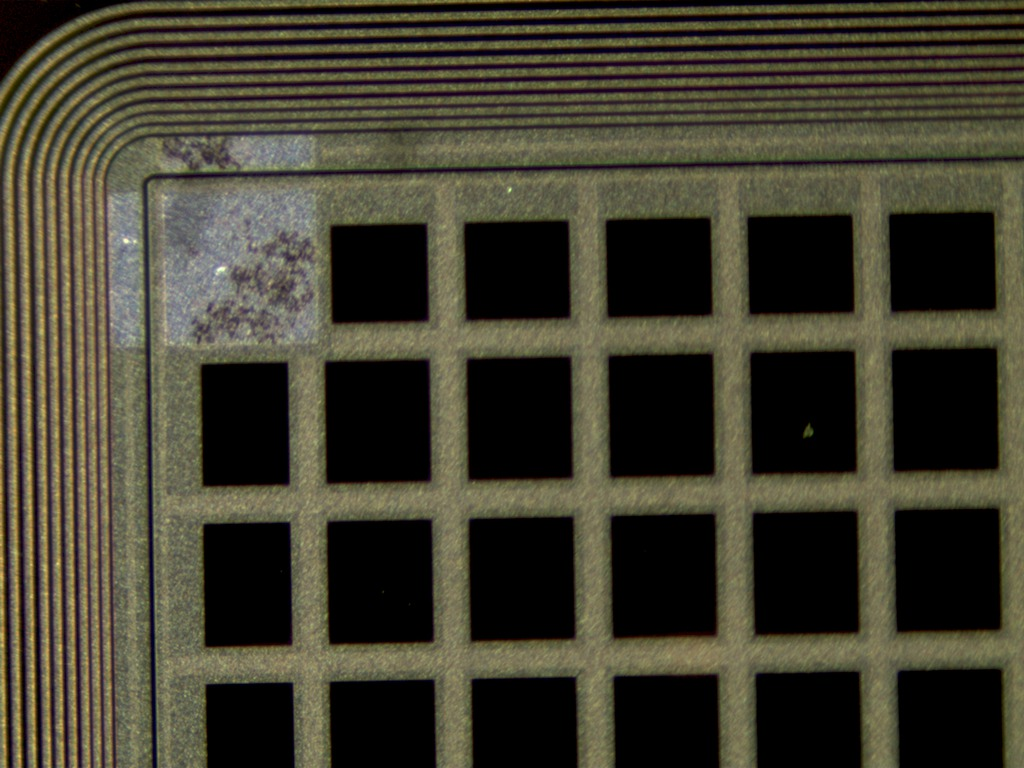
\includegraphics[width=0.4\textwidth]{ch7/vis_insp_2}
	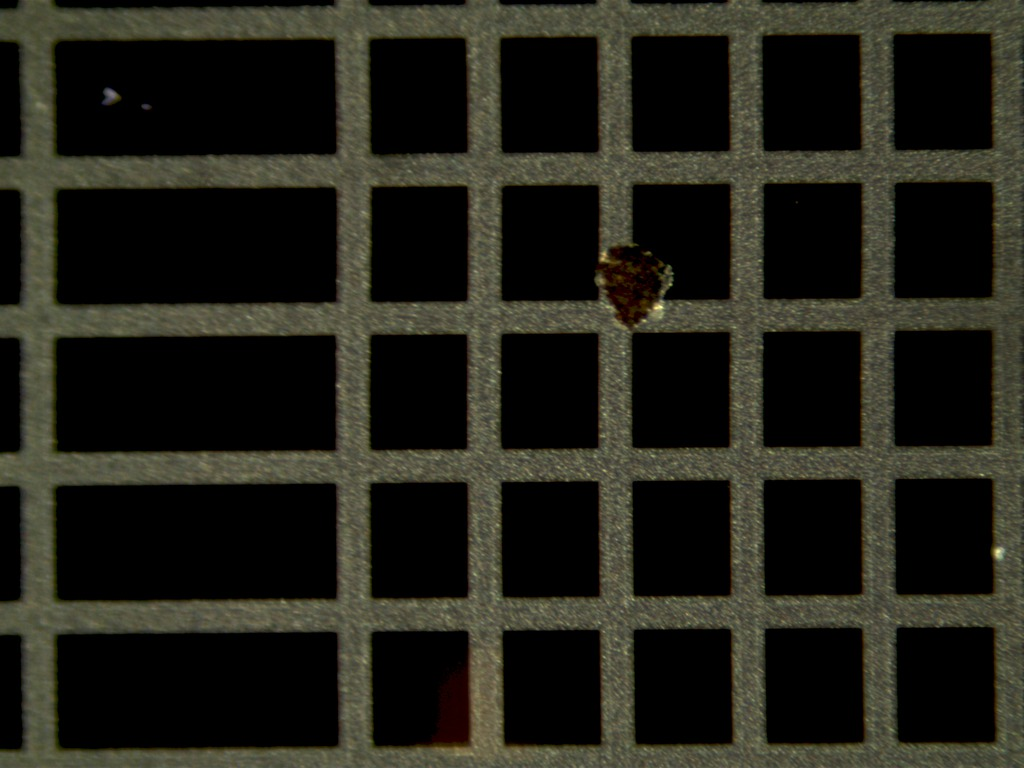
\includegraphics[width=0.4\textwidth]{ch7/vis_insp_3}
	\caption[Visual inspection of a bare module.]{Photograph of the visual inspection of a BBM showing few of the things observed during a visual inspection: A good module (top left), chipped ROC (top right), scratches on the high voltage connection pad (bottom left), and scratch on the midle of a ROC (bottom left)}
	\label{fig:vis_insp_bbm}
\end{figure}

\begin{figure}[!h]
	\centering
	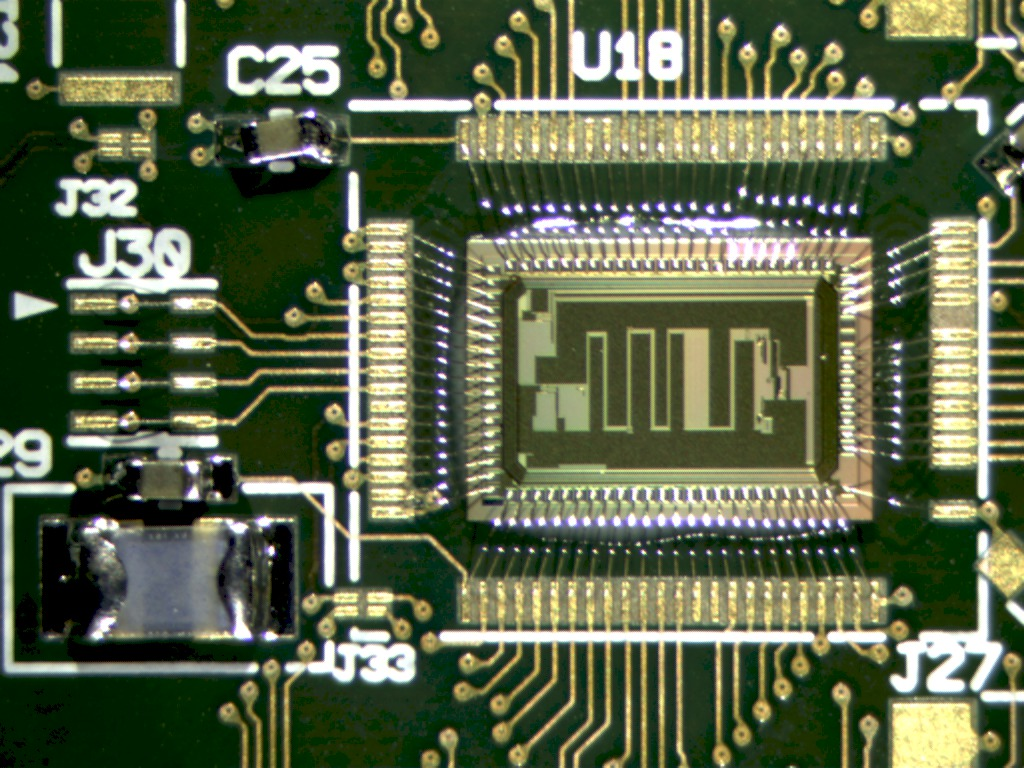
\includegraphics[width=0.4\textwidth]{ch7/hdi_tbm}
	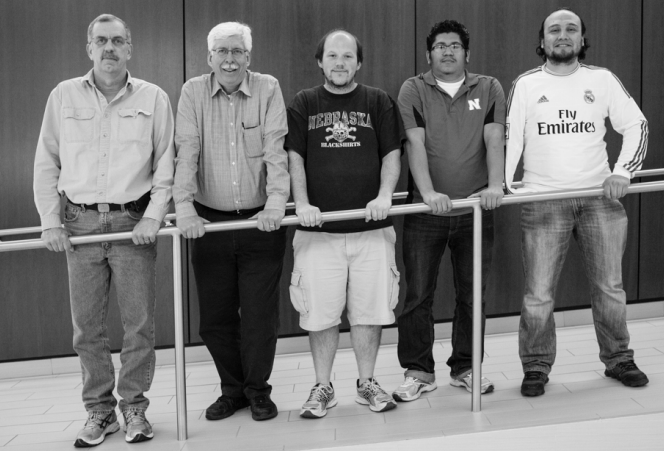
\includegraphics[width=0.4\textwidth]{ch7/aaaa}
	\caption[Visual inspection of a HDI.]{Photograph of the visual inspection of a HDI shwing the wirebonds of the TBM (left) and the bondpads of a ROC (right). {\rojo{right fig}}}
	\label{fig:vis_insp_hdi}
\end{figure}

Figures \ref{fig:vis_insp_bbm} and Fig. \ref{fig:vis_insp_hdi} also show a trend that was observed throughout the entire production phase. In general more unusual features and damage were observed in BBMs than on HDI. This was because BBM were derivered directly from the production company to our lab while HDIs were first delivered to the Fermi National Laboratory (FermiLab) where they were preliminary tested and inspected before they arrive at our testing facilities. 

\subsection{IV Test}\label{ivbbm}
After both BBM and HDI have succesfully passed the visual inspection the BBM continues to the probe station for a current vs voltage (IV) test. The test uses the fact that the sensor behaves like a diode. During operation a potential difference is applied to the sensor to draw the electrons created by a charge particle passing through the sensor towards the bump bond to be collected. If this potential difference is too small not all electron will collected in time and if it is large the sensor could break. This potential difference is known as a depletion voltage. The IV test is meant to find the operating range, a voltage where all the electron could be collected and the sensor will not break, for a given module (sensor). Figure \ref{fig:sensor_probe_positions} (left) shows the position of the probes to perform an IV on a BBM and figure \ref{fig:sensor_probe_positions} (right) shows IV results for a BBM in good operating condition.  

\begin{figure}[!h]
	\centering
	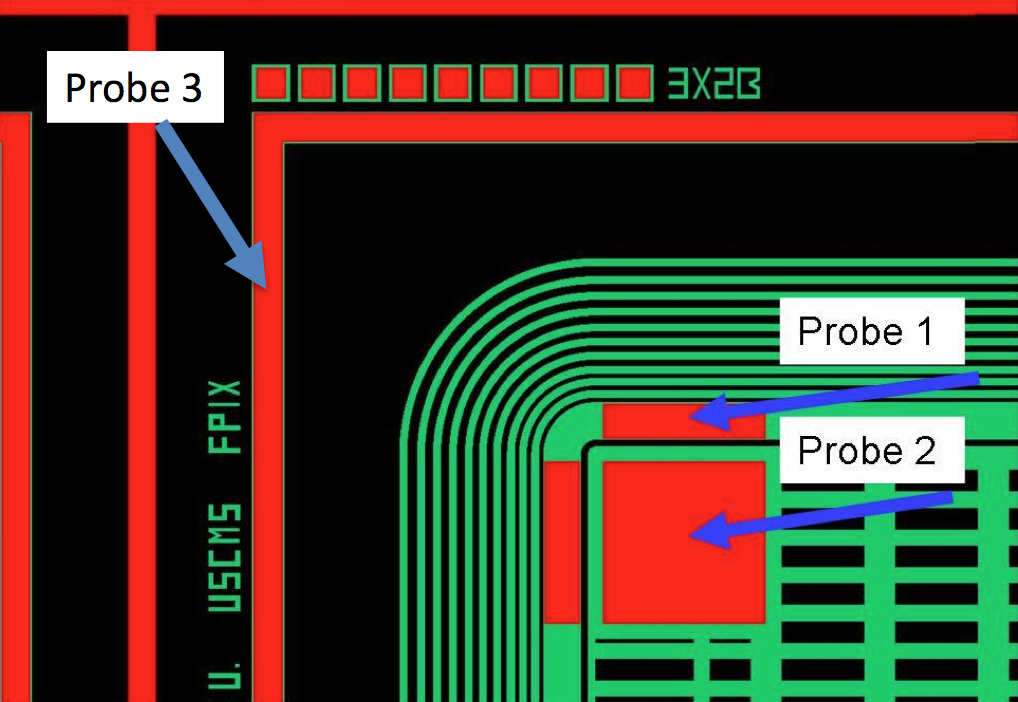
\includegraphics[width=0.5\textwidth, height= 0.42\textwidth]{ch7/sensor_probe_positions}
	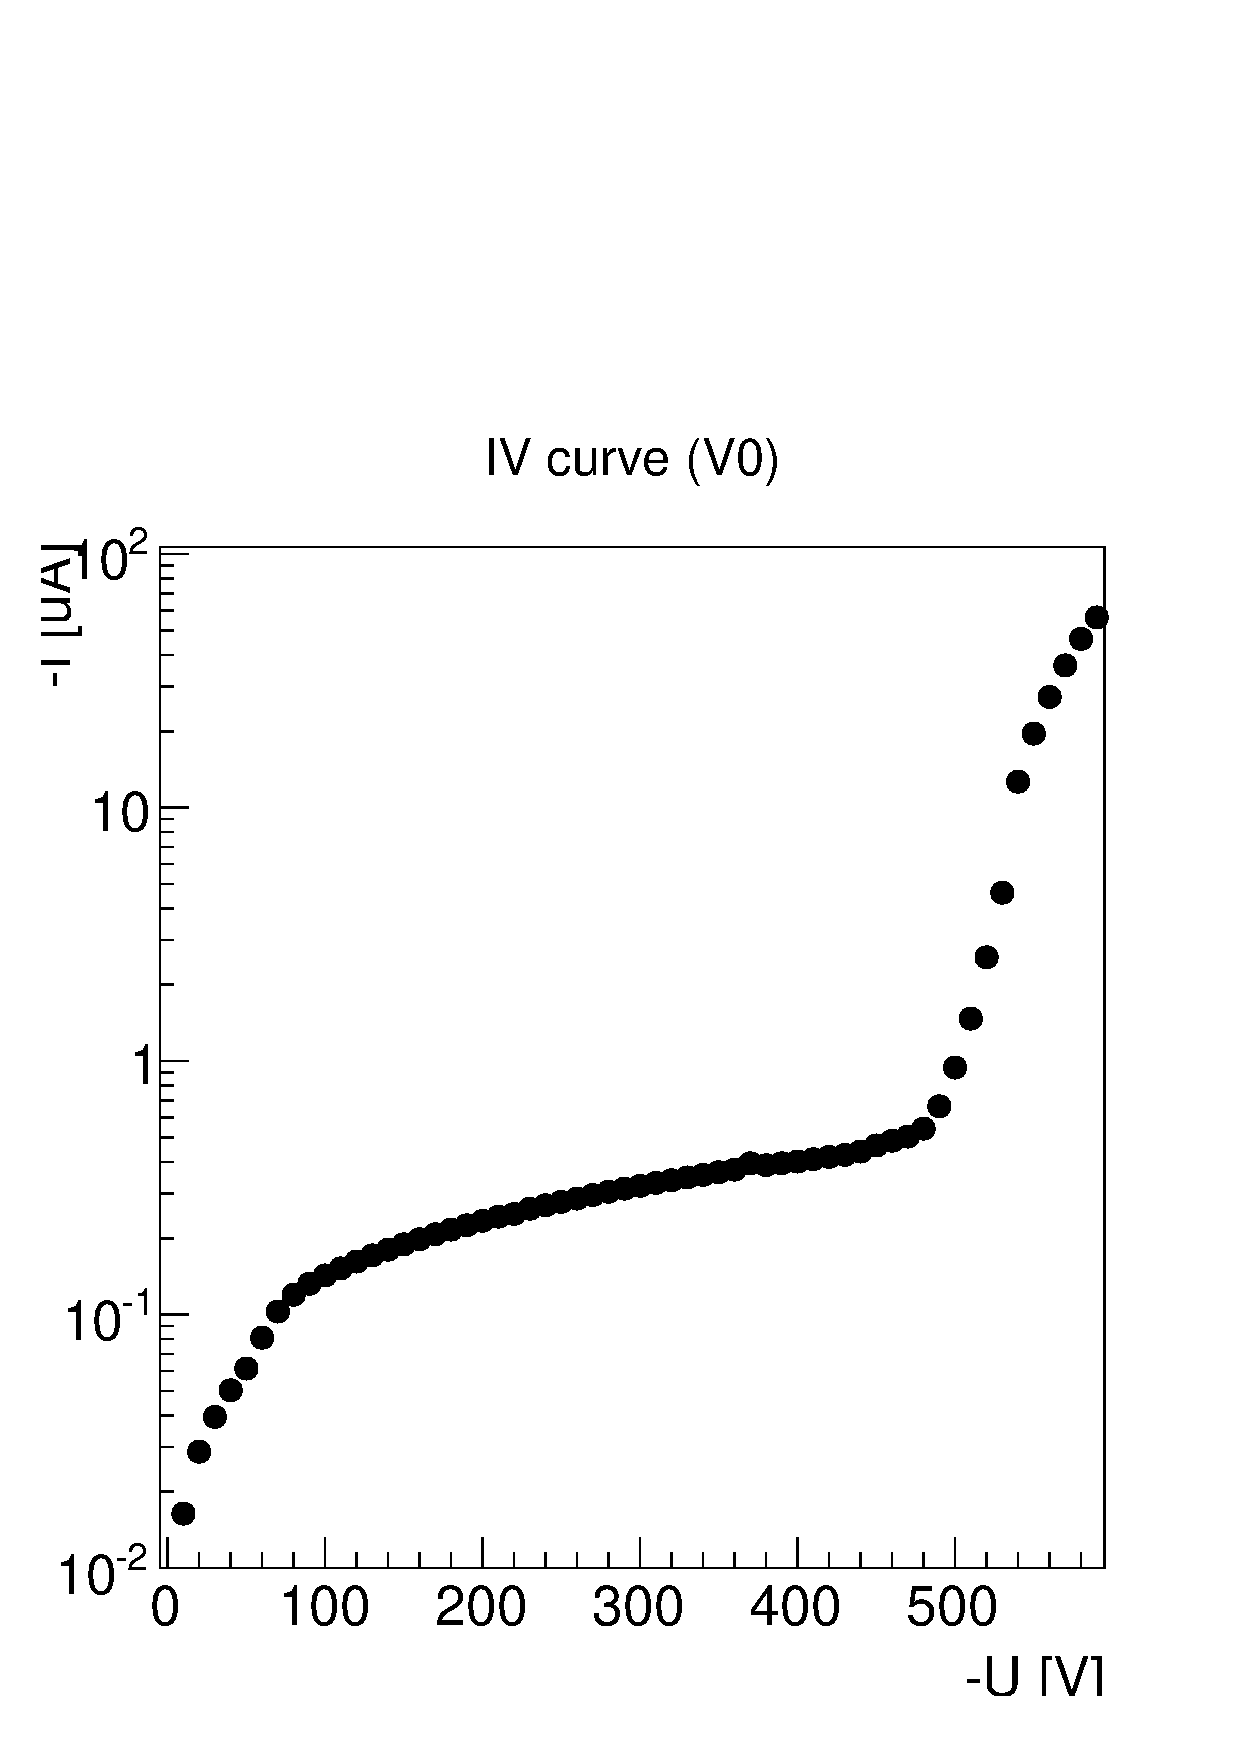
\includegraphics[width=0.4\textwidth]{ch7/iv_test}
	\caption[IV test of BBM]{Left: Probe position for an IV test on a BBM. Probe 2 is high voltage, probe 3 is ground, and probe 1 was not used \cite{ph1_sop}. Right: IV test results for a good BBM. The depletion voltage for this module is around {\rojo{confirm with right picture}}.}
	\label{fig:sensor_probe_positions}
\end{figure}

\subsection{Gluing}
The gluing routine was carefully design to perfectly match the HDI and BBM bondpads, in preparation for the wirebonding. This stage of the production was done using a custom made gantry, \ital{AGS15000 Series Gantry}, fabricated by Aerotech \cite{aerotech}. It offered translational motion in 3D as well as rotation in x-y (gantry table) plane. A camera was attached to the gantry head allowing the user to monitor the entire process. This camera was of particular importance during the development and improvement of the gluing and encapsulation routine. A video showing the gluing routine in action can be watched at \cite{gluing_frank} and a full description of the gluing routine and procedure can be found in \cite{and_the}. Figure \ref{fig:gantry} shows the gantry with the different tools used to glue a HDI on a BBM. The final product after the process is completed can be seen in Fig. \ref{fig:hdionbbm}.

\begin{figure}[!h]
	\centering
	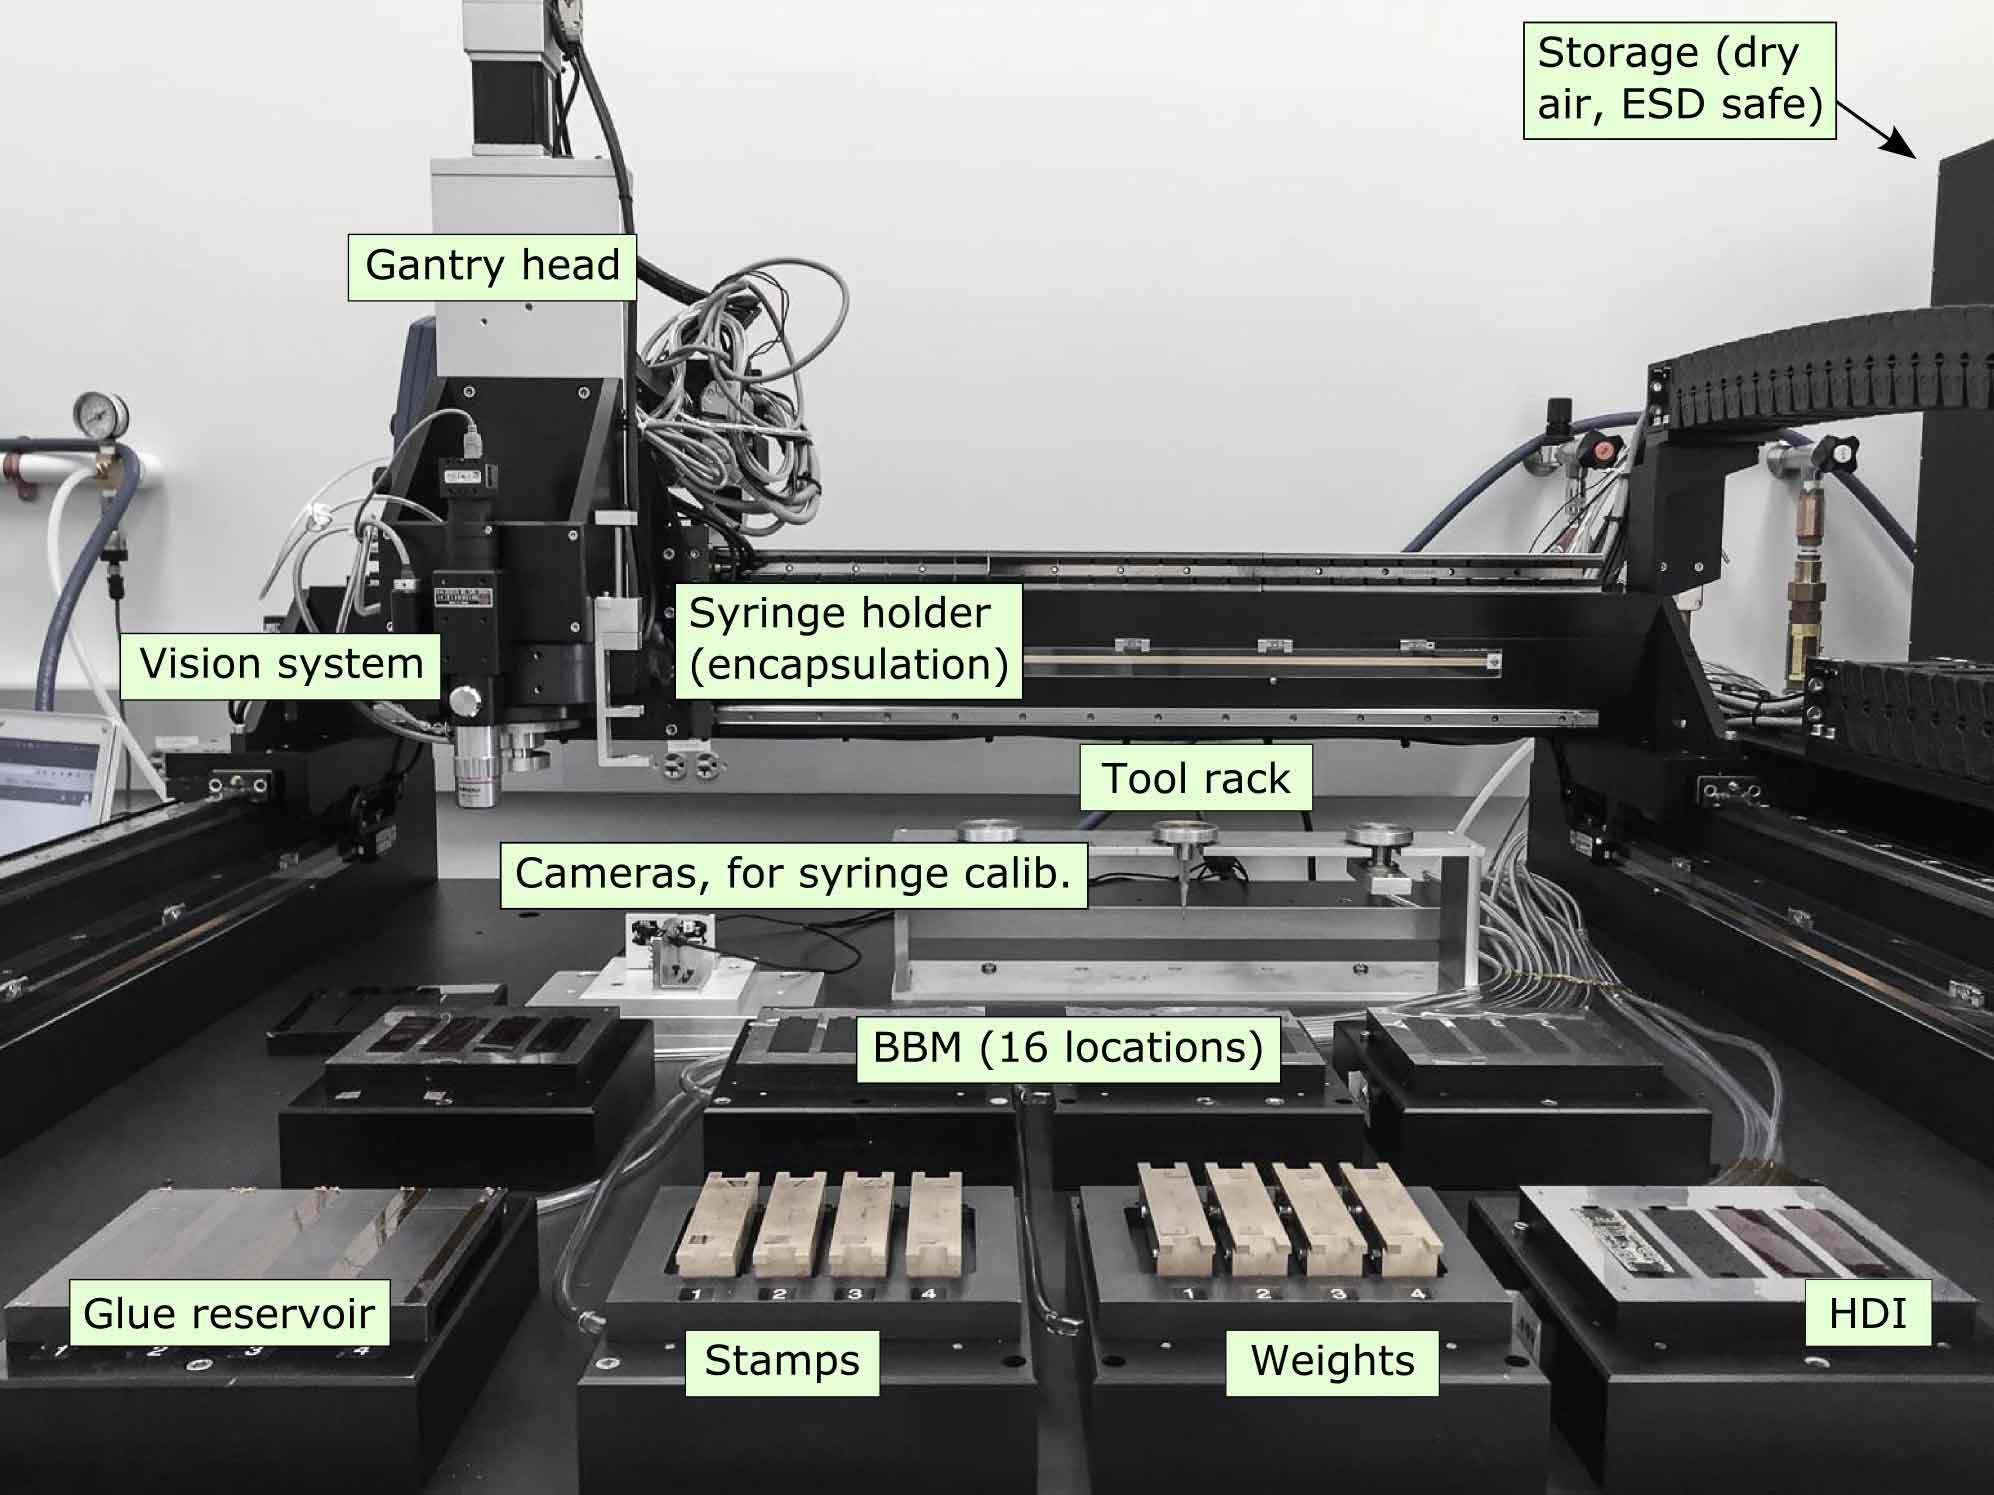
\includegraphics[width=0.7\textwidth]{ch7/gantry}
	\caption[Gluing and encapsulation set up]{Photograph of a gantry used for gluing and encapsulation showing different parts of the set up and tools. }
	\label{fig:gantry}
\end{figure}

\begin{figure}[!h]
	\centering
	\includegraphics[width=0.5\textwidth]{ch7/hdi_on_bbm}
	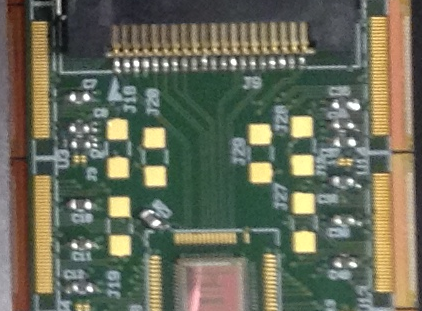
\includegraphics[width=0.5\textwidth]{ch7/hdi_on_bbm_close}
	\caption[Gluing result]{HDI glued on top of a BBM. For a batch of four modules (top) and zoom in view to note the almost perfect alignment between the HDI and BBM bondpads.}
	\label{fig:hdionbbm}
\end{figure}


\subsection{Wirebonding}
After an HDI is glued to a BBM the next step in the assembly process is to make electrical connection between them. To this end, a wirebonder machine, Delvotec 56XX, and aluminium wires of 25\,$\mu$m diameter were used. {\rojo{need more}}

Figures \ref{fig:wirebonder}, \ref{wirebondinaction} and \ref{fig:wirebond} show the set up the process and the final product respectively 
\begin{figure}[!h]
	\centering
  	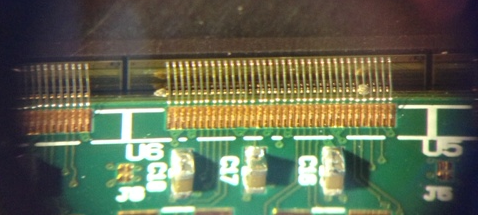
\includegraphics[width=0.7\textwidth]{ch7/wirebonder}
  	\caption[wirebonder machine]{Wirebonding set up {\rojo{find good picture of the wirebonder}}.}
  	\label{fig:wirebonder}
\end{figure}


\begin{figure}[!h]
	\centering
  	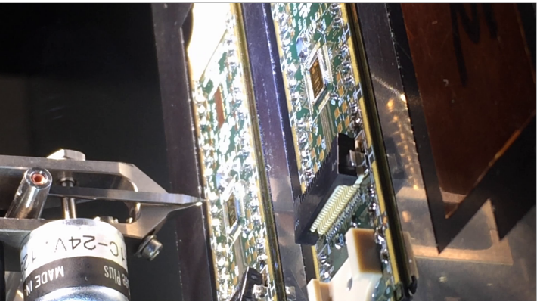
\includegraphics[width=0.7\textwidth]{ch7/wire_bond_fig}
  	\caption[wirebonder process]{Wirebonder in action with a batch of two modules \cite{brian_disc}.}
  	\label{wirebondinaction}
\end{figure}


\begin{figure}[!h]
  	\centering
  	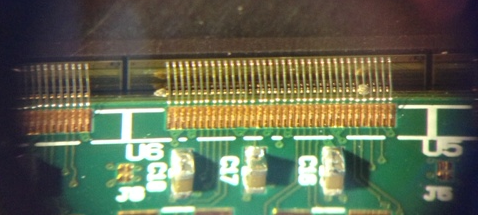
\includegraphics[width=0.7\textwidth]{ch7/wirebond}
  	\caption[Wirebonded module]{Close up view of the wirebonds for a single ROC on a wirebonded module.}
  	\label{fig:wirebond}
\end{figure}



\subsection{Encapsulation}
The final step in manufacturing a module is to protect (cover) the wirebonds with an encapsulant, wirebond encapsulation. This procedure is necessary to ensure that the wirebonds are secure at both HDI and BBM ends. The set up and the equipment used is the same as for gluing showed in figure \ref{fig:gantry}. Additional materials needed for this step are shown in figure \ref{fig:encapmate}. 
 
\begin{figure}[!h]
	\centering
	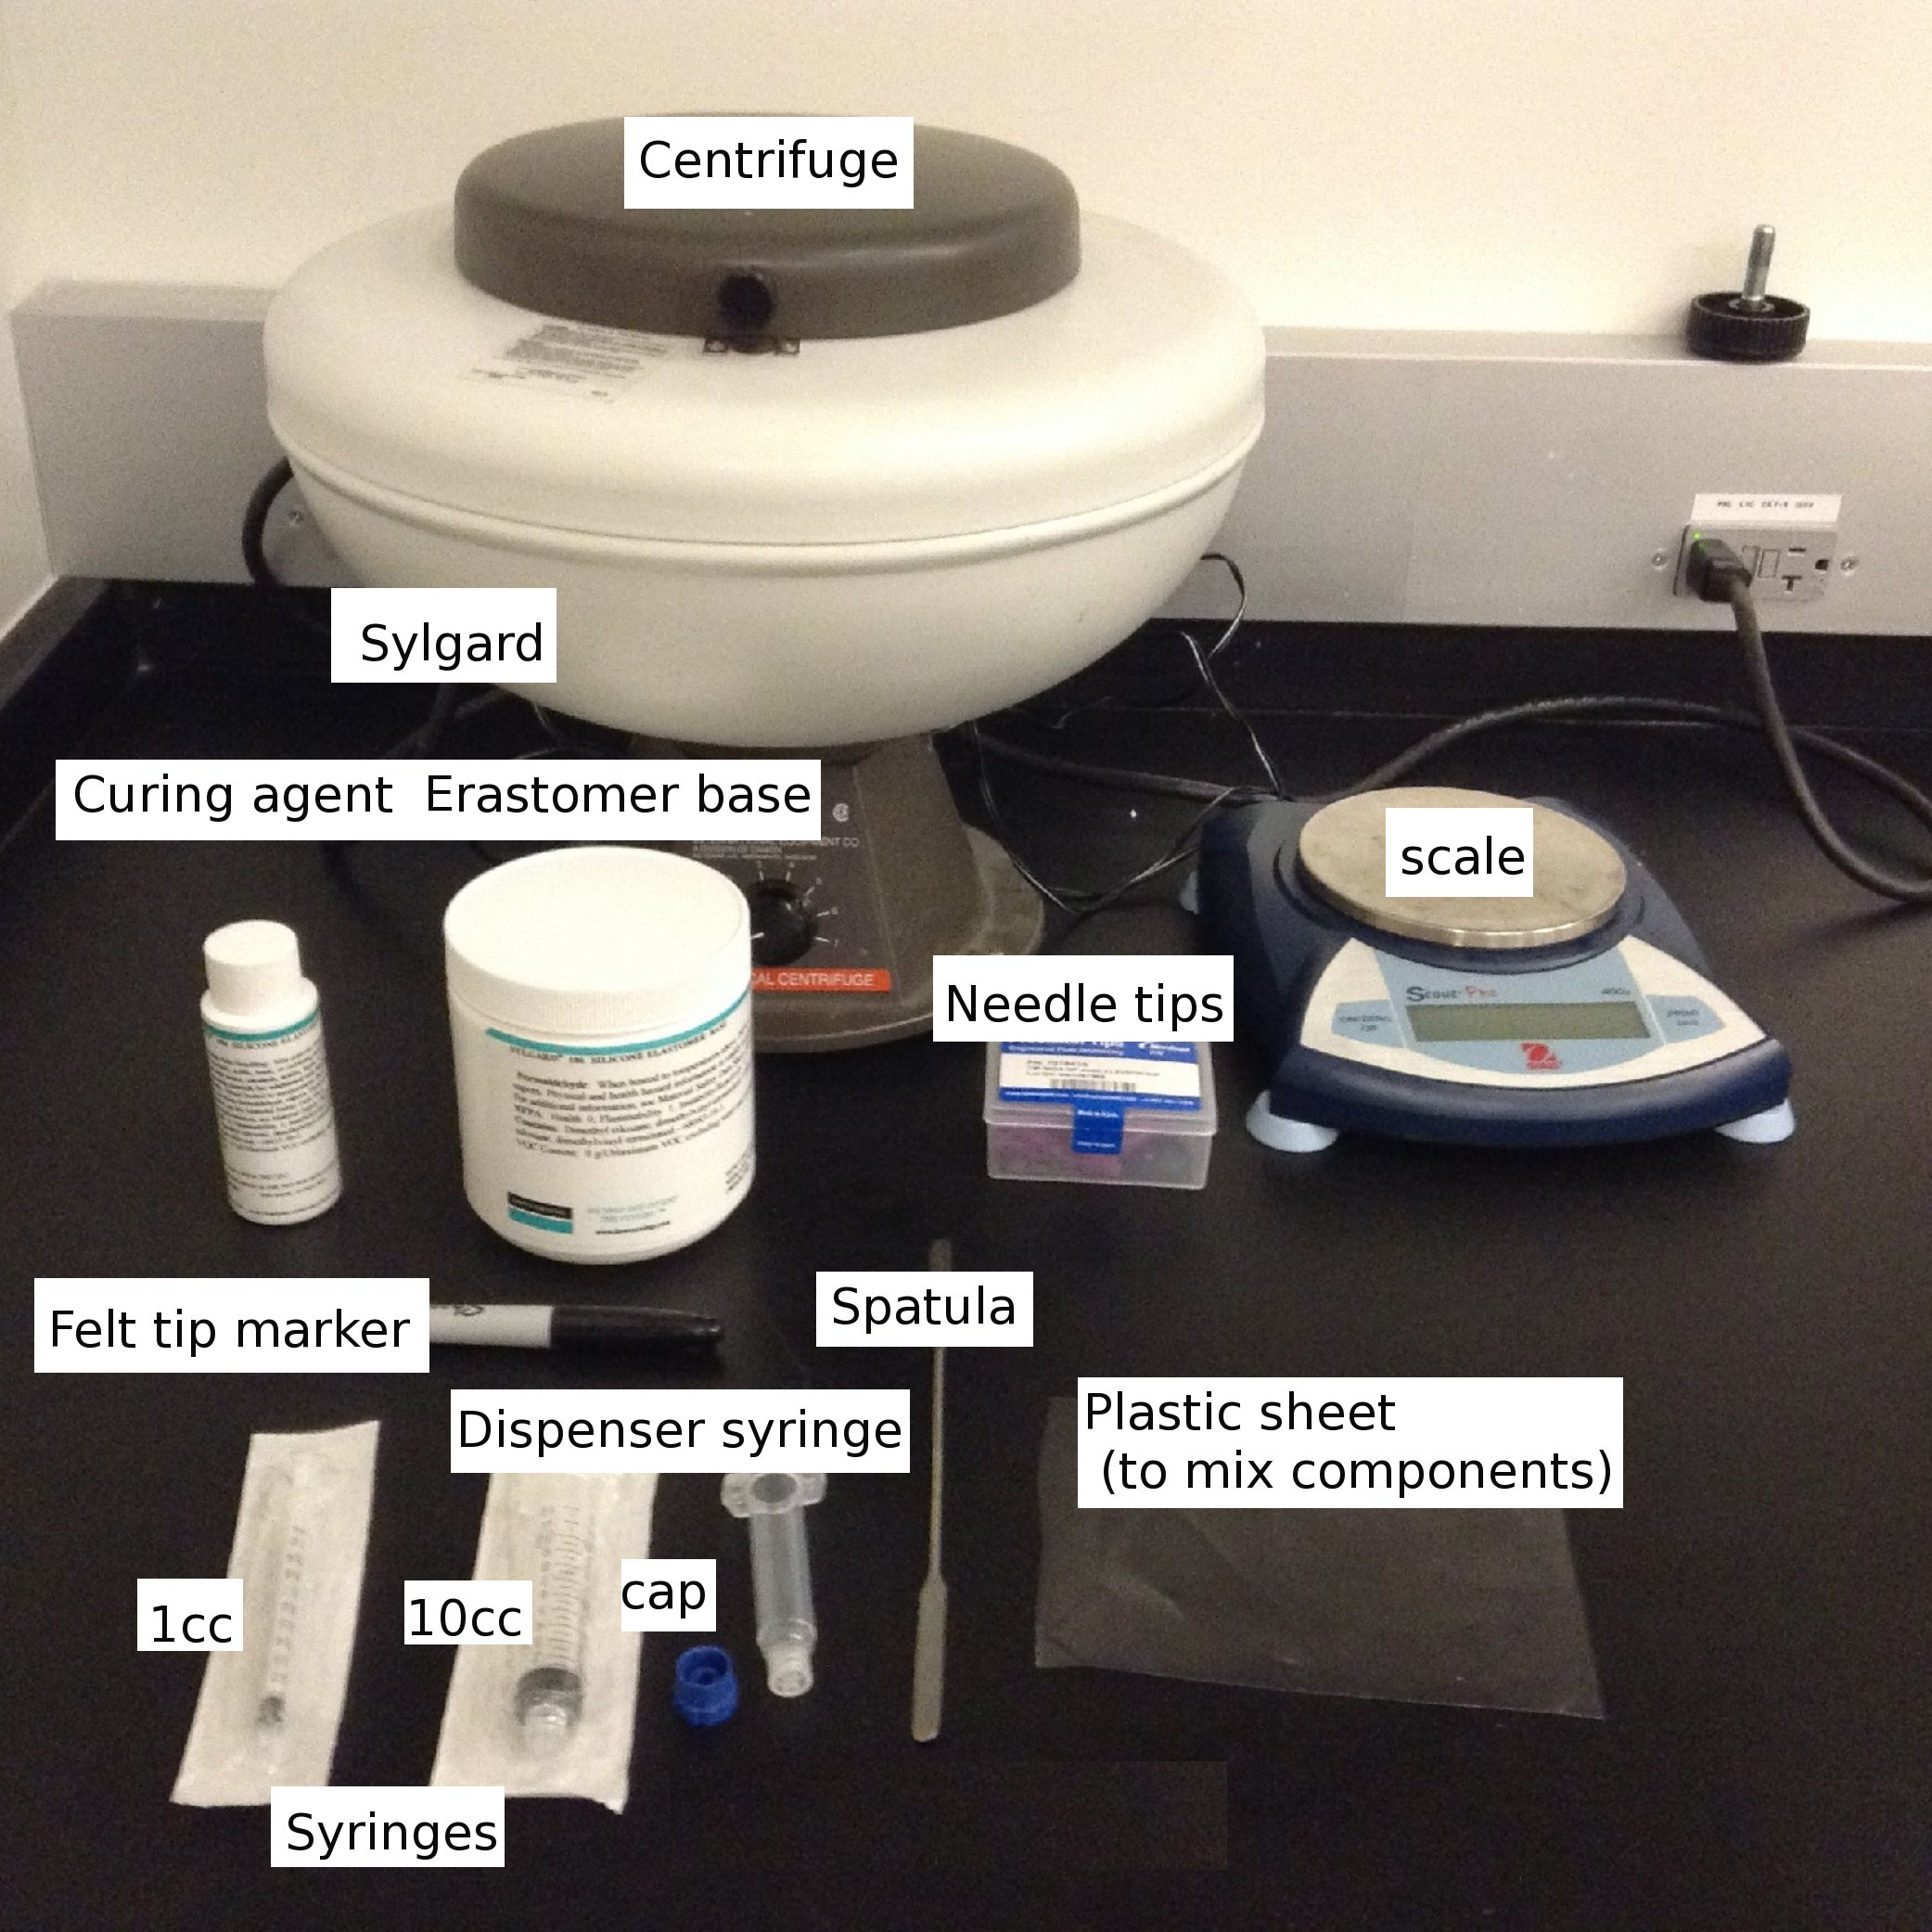
\includegraphics[width=0.5\textwidth]{ch7/encap_mat}
	\caption[Encapsulation materials]{Wirebonds encapsulation materials \cite{ph1_sop}.}
	\label{fig:encapmate}
\end{figure}

A material suitable for this task must be radiation hard and lightweight among other properties. After testing different material and alloys we settle on \ital{Silgard 186}, a mixture of two-component encapsulant. Erastomer (10 cc) and elastomer (1 cc) base and curing agent respectively. The components then, were mix together using a centrifuge and place in a syringe for dispensing. There are three components that need encapsulation, HDI and BBM bond pads, TBM wirebonds, and high votage pads. Figure \ref{fig:encap} shows a module after its different components have been encapsulated. Note how all bond foots and pads are fully covered as needed \cite{and_the}. 

\begin{figure}[!h]
  \centering
  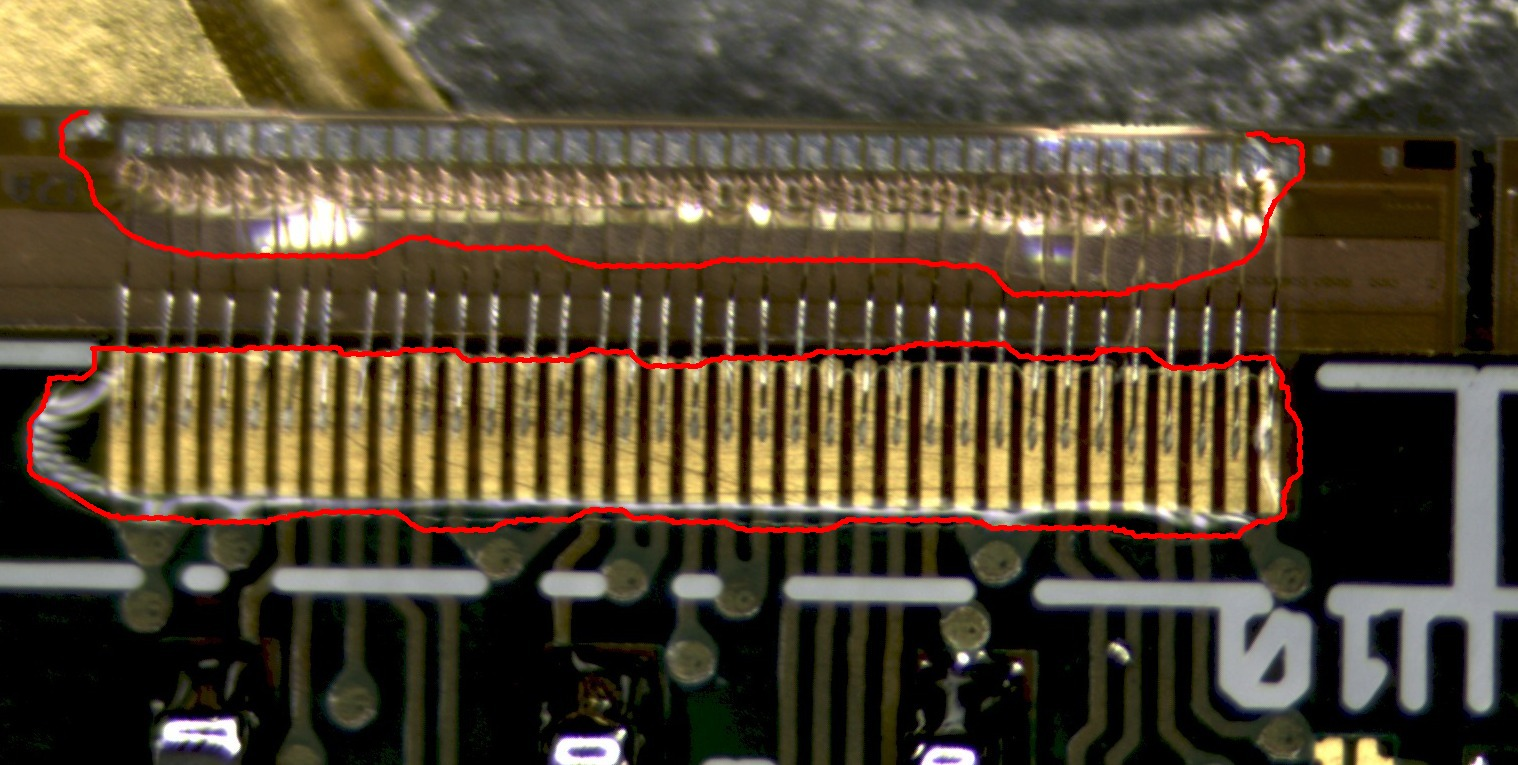
\includegraphics[width=0.5\textwidth]{ch7/encap_ref}
  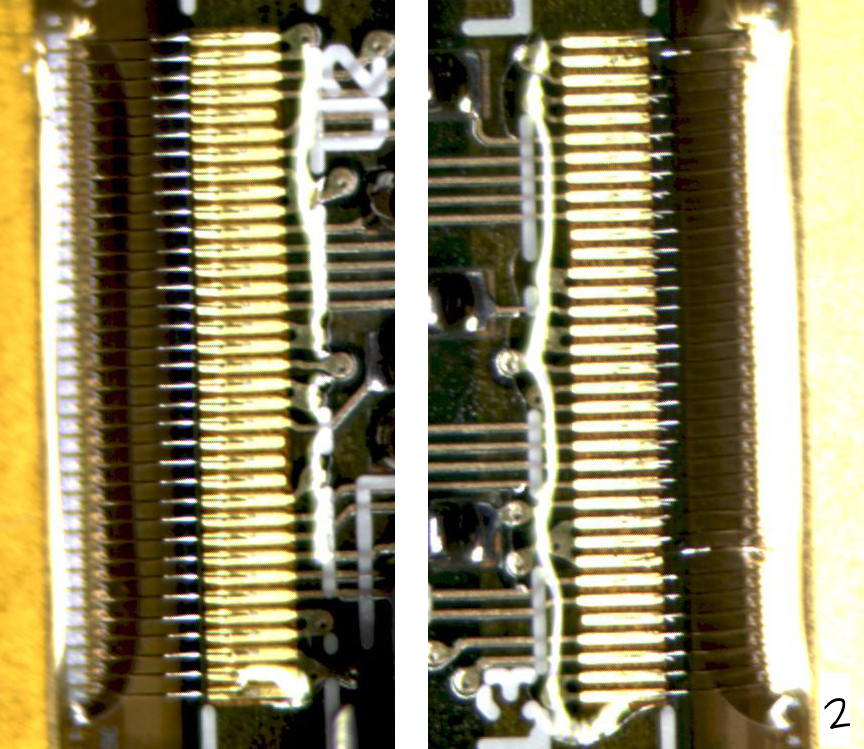
\includegraphics[width=0.4\textwidth]{ch7/encap_roc}
  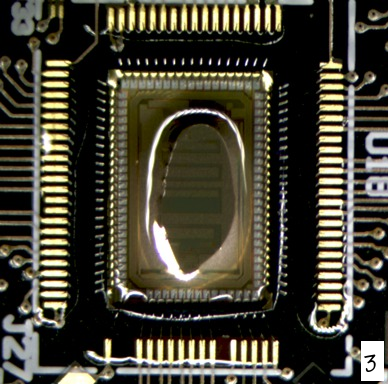
\includegraphics[width=0.2\textwidth]{ch7/encap_tbm}
  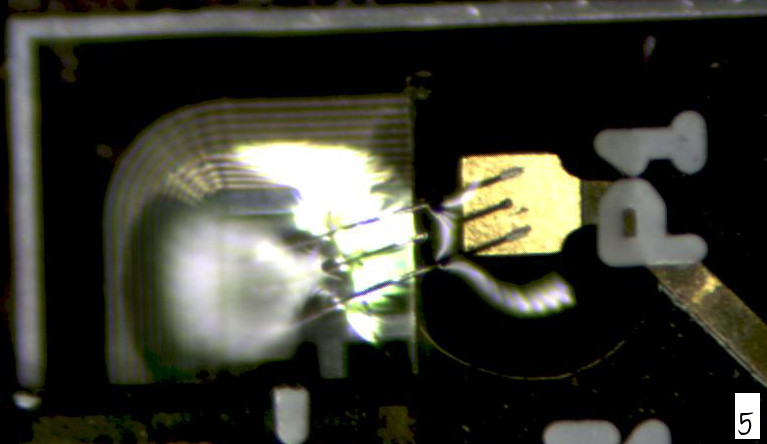
\includegraphics[width=0.4\textwidth]{ch7/encap_hv}
  \caption[Encapsulation results]{Wirebonds encapsulation of the components of a module. Top left, roc used as reference, the boundaries of the encapsulant are enhanced with red lines for better visibility. Top right, two ROCs on two different modules side by side, b) encapsulation of TBM, c) encapsulation of the high voltage pad.}\label{fig:encap}
\end{figure}

\subsection{Electrical Test of a Fully assembly Module}
A manufactured module can be seen in Figure \ref{fig:fully_asem_mod}, it is then visually inspected and mark as ready for electrical test {\rojo{at the end of previous session?}}. 
The electrical test, hereon fulltest, of fully assembly modules is done using the \ital{pXar} software framework, written by the CMS FPix collaboration. More information on \ital{pXar} can be found in \cite{pxar}. The objective of the \ital{Fulltest} is to ensure that all 16 ROCs were functional and have good performance. For this purpose a suit of several tests were designed and developed, the software is flexible in the sense that we could execute a single test just by calling its name or we could execute them all with a single command \ital{Fulltest} with the exception of the IV test. The \ital{Fulltest} at UNL was done using the set up showing in figure \ref{cold_box} at a temperature of $17^{\circ}$ $C$ and using a depletion voltage of $-150$ $V$. The set up allowed us to test up to 4 modules in parallel using a software called \ital{ElComandante} \cite{elcomandante} written specifically for this purpose. The modules are connected via flex cables to adapter cards which convert the data into SCSI format. Each adapter card is connected to a digital test board and the data is finally transferred to a computer via an USB cable. The temperature inside the colbox was controlled by a chiller.

\begin{figure}[!h]
	\centering
	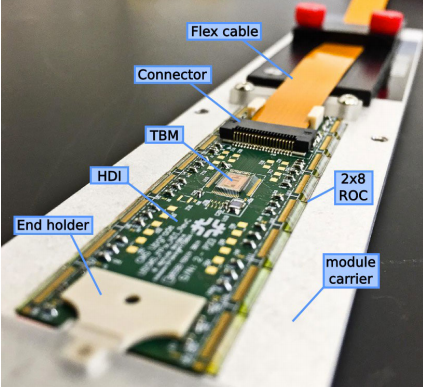
\includegraphics[width=0.7\textwidth]{ch7/fully_asem_mod}
	\caption[Fully assembly Module]{Fully assembly Module}
	\label{fig:fully_asem_mod}
\end{figure}

\begin{figure}[!h]
	\centering
	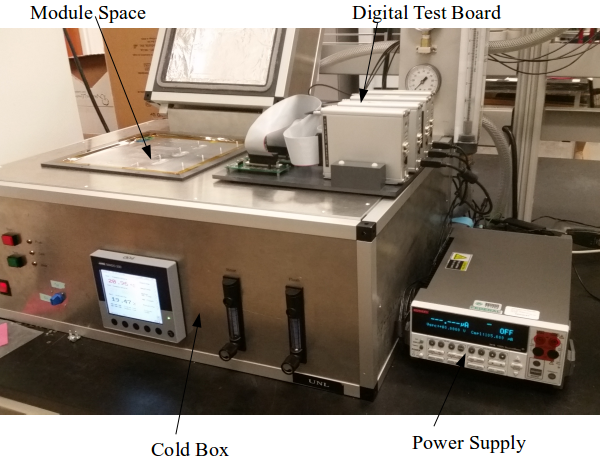
\includegraphics[width=0.7\textwidth]{ch7/cold_box}
	\caption[Testing set up]{Fully assembly module testing set up}
	\label{cold_box}
\end{figure}

The following section {\rojo{subsections?}} give a short description of the most \ital{important} tests a module has to surpass as well as the output of these test. A full list of the tests, a comprehensive description of them, and a {\rojo{description}} of their purpose can be found in \cite{fpix_module_testing_guide} and references therein. After the \ital{Fulltest} of modules was completed some were shipped to Kansas university for X-ray testing and the rest were shipped to FermiLab for testing at $-10^{\circ}$ $C$

\subsubsection{IV Test}
A fully assembled module also undergoes an IV test as described in \ref{ivbbm}. The primary purpose of this test is to ensure that not damage was caused to the circuitry during the assembly process and the module could be operated at high voltages. The IV result for a sample module is shown in figure \ref{ivfullmod}. The operational range for this particular module is between -100 V and -400 V.

\begin{figure}[!h]
	\centering
	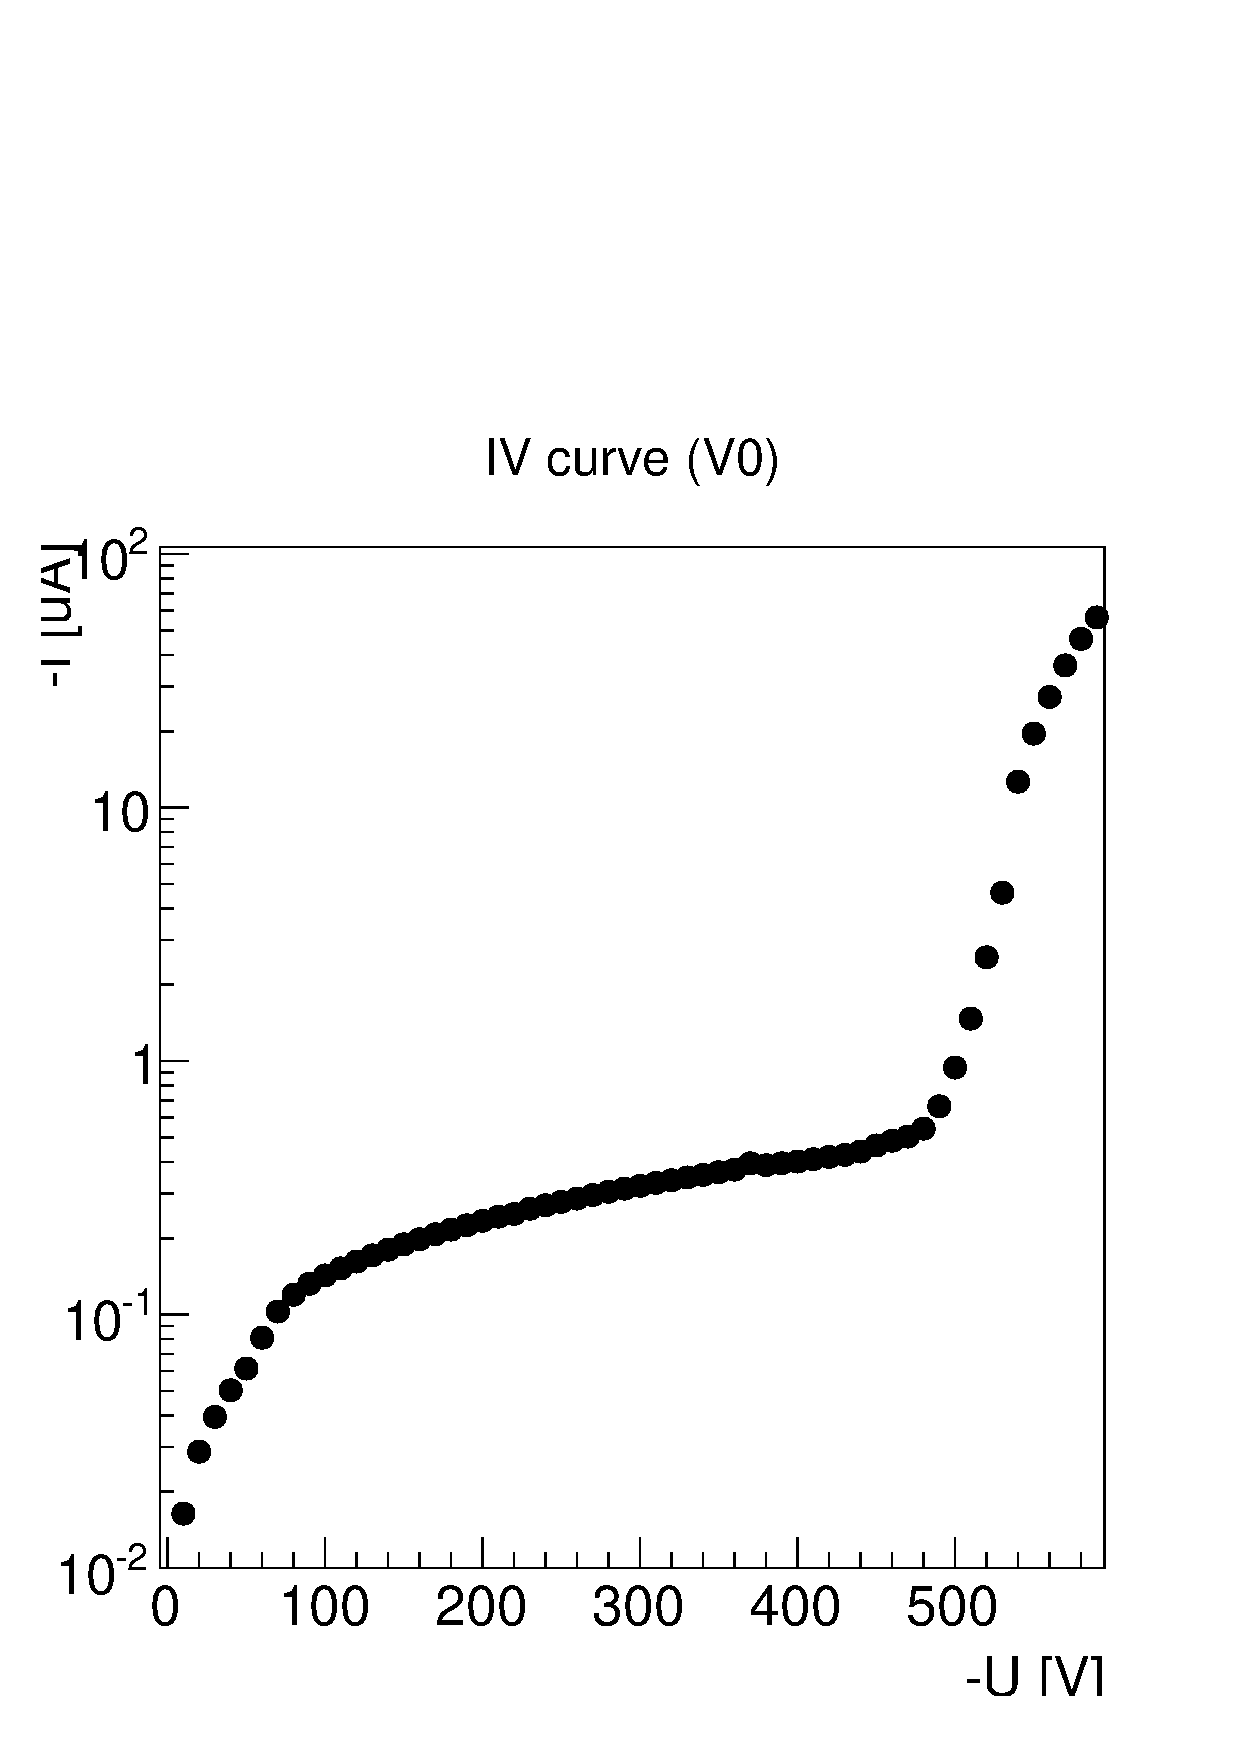
\includegraphics[width=0.4\textwidth]{ch7/iv_test}
  	\caption[IV results of a module]{IV test for a fully assembly module.}
  	\label{ivfullmod}
\end{figure}

\subsubsection{Pretest}
It is composed of several subtests and its purpose is to check the basic functionalities of the ROCs and to calibrate some of the DAC {\rojo{list of DAC here or in ch 2?}} settings. A couple of these subtests are \ital{ProgramRoc} and \ital{SetVthrCompCalDel}. The \ital{ProgramRoc} measures the difference in current (Iana) drawn by the amplifiers when a voltage (Vana) is applied and remove. 
If the difference between these two measurements is non-zero it implies that we are able to change DAC values by sending a command, the ROC is programmable. This test is done for all 16 modules in a ROC. The \ital{SetVthrCompCalDel} subtest is done to optimize the value of the VthrComp and CalDel DACs. It chooses a pixel from within a ROC and sends 5 calibration pulses to the PUC of this pixel. This process is repeated for the 256 x 256 parameter space of these DACs and the response of the pixel is read to make an efficiency plot. Then VthrComp is set to the lower plateau plus 50 units and CalDel is set to half of the left and right edges. This is known as the \ital{VthrComp} and \ital{CalDel} working point of the pixel. Figure \ref{fig:pretest} shows the output of these subtests for a sample module

\begin{figure}[!h]
  \centering
  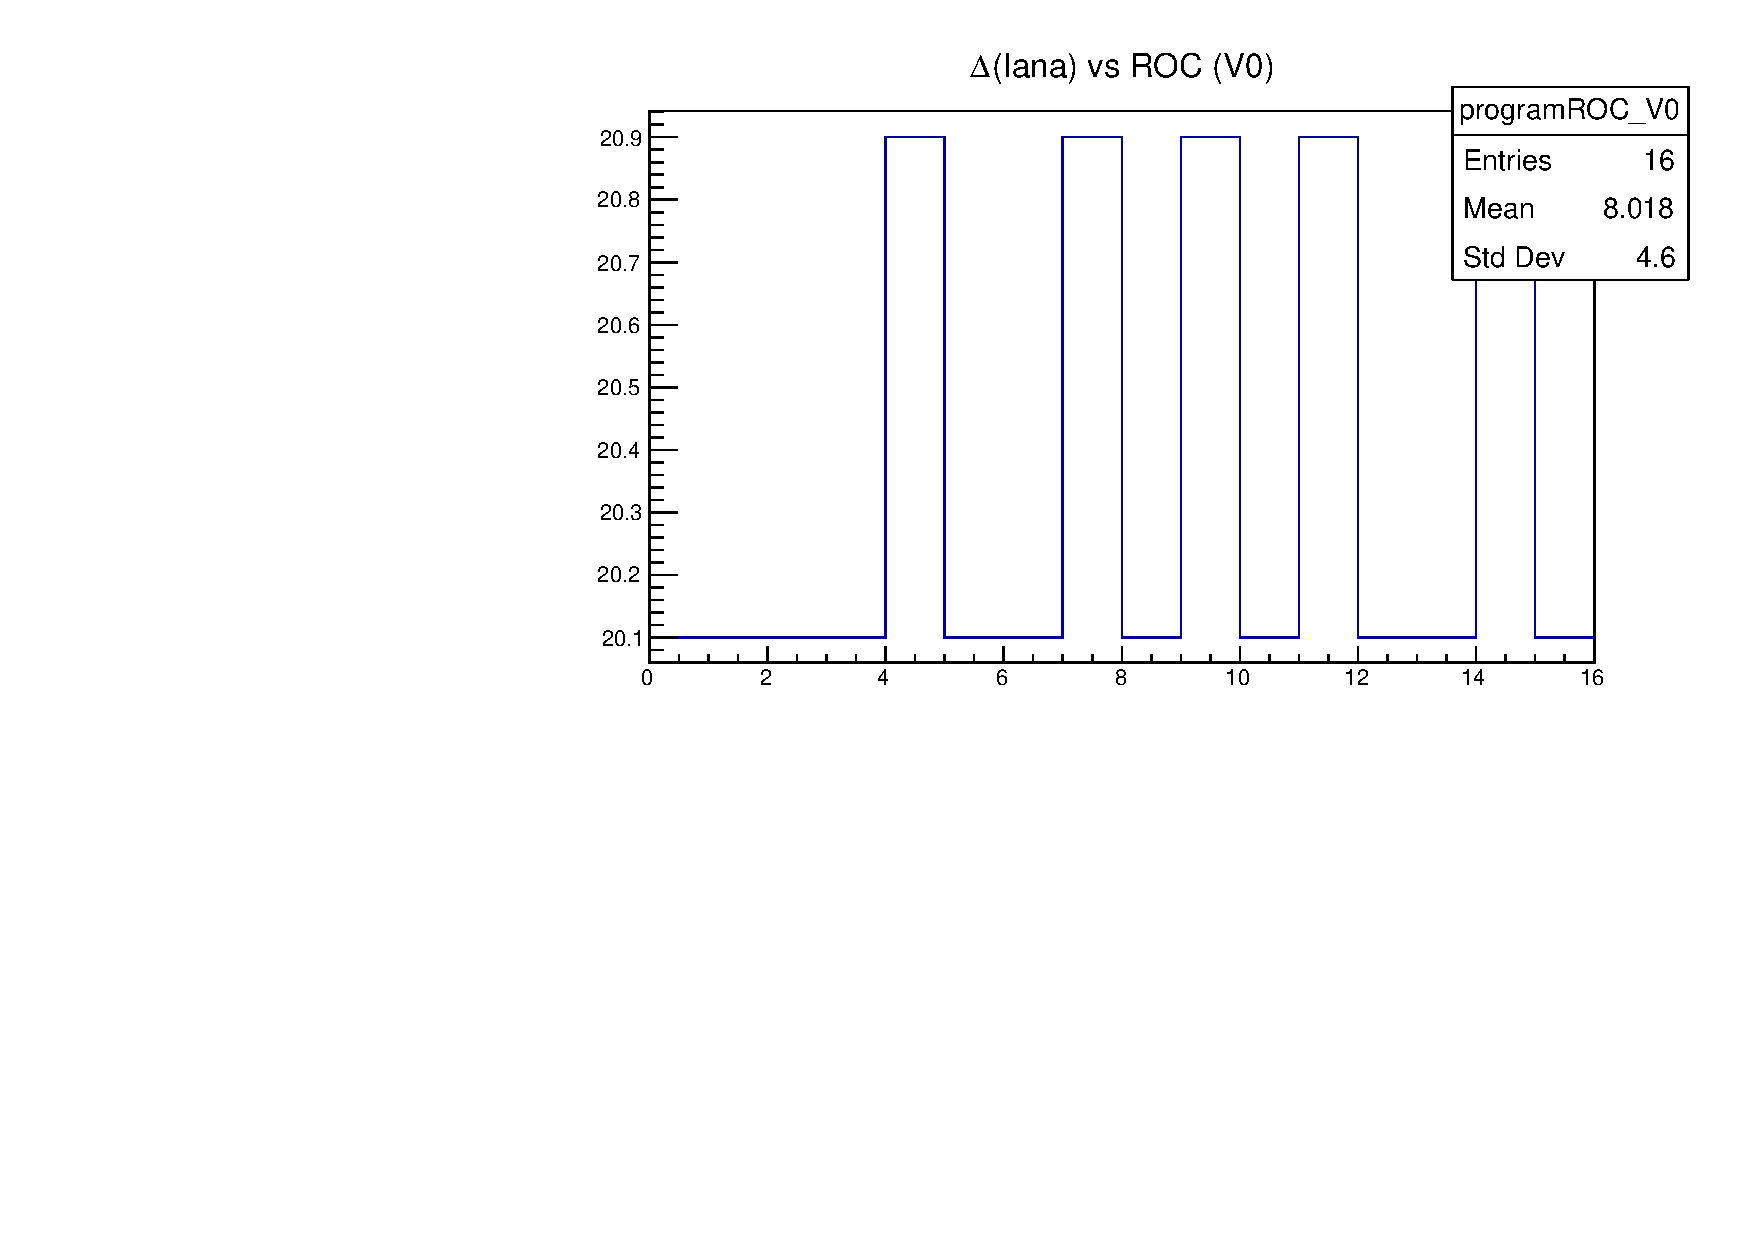
\includegraphics[width=0.7\textwidth]{../images/ch7/pro_roc}
  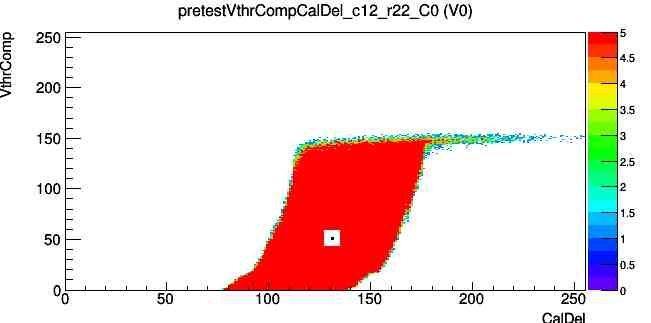
\includegraphics[width=0.7\textwidth]{../images/ch7/working_point}
  \caption[Programable ROC and working point]{Output of the ProgramRoc (left) and finding working pixel (right) subtests.}\label{fig:pretest}
\end{figure}

\subsubsection{Pixel Alive}
In the pixel alive test three subtests are performed: \ital{Alive test} checks for the response of a pixel by sending 10 calibration pulses (hits) to it and recording how many the pixel reports back. Pixel with 10 hits are marked as good, those with less than 10 hits are flagged as faulty, and those with zero hits are called dead. In the \ital{Mask test} all pixels are disable and the same efficiency measurement is done. Pixels with zero efficiency are marked as good while those with efficiency grater than zero are bad. The \ital{AddressDecoding} test checks the specific address of the pixel within the ROC. If the response of the pixel does not match the address to which it was sent the pixel if marked as bad. repeats the same procedure but checks that the order of the resulting data. If the address of a given pixel is out
of order, the recorded hit is given a negative pulse height value. Pixels with negative
hits are flagged as faulty. Figure \ref{fig:pix_ali} shows the result of the pixel alive test for a fully working module and Figure \ref{fig:pix_ali_bad} shows a module with faulty ROC and a ROC with faulty pixels. 

\begin{figure}[!h]
  \centering
   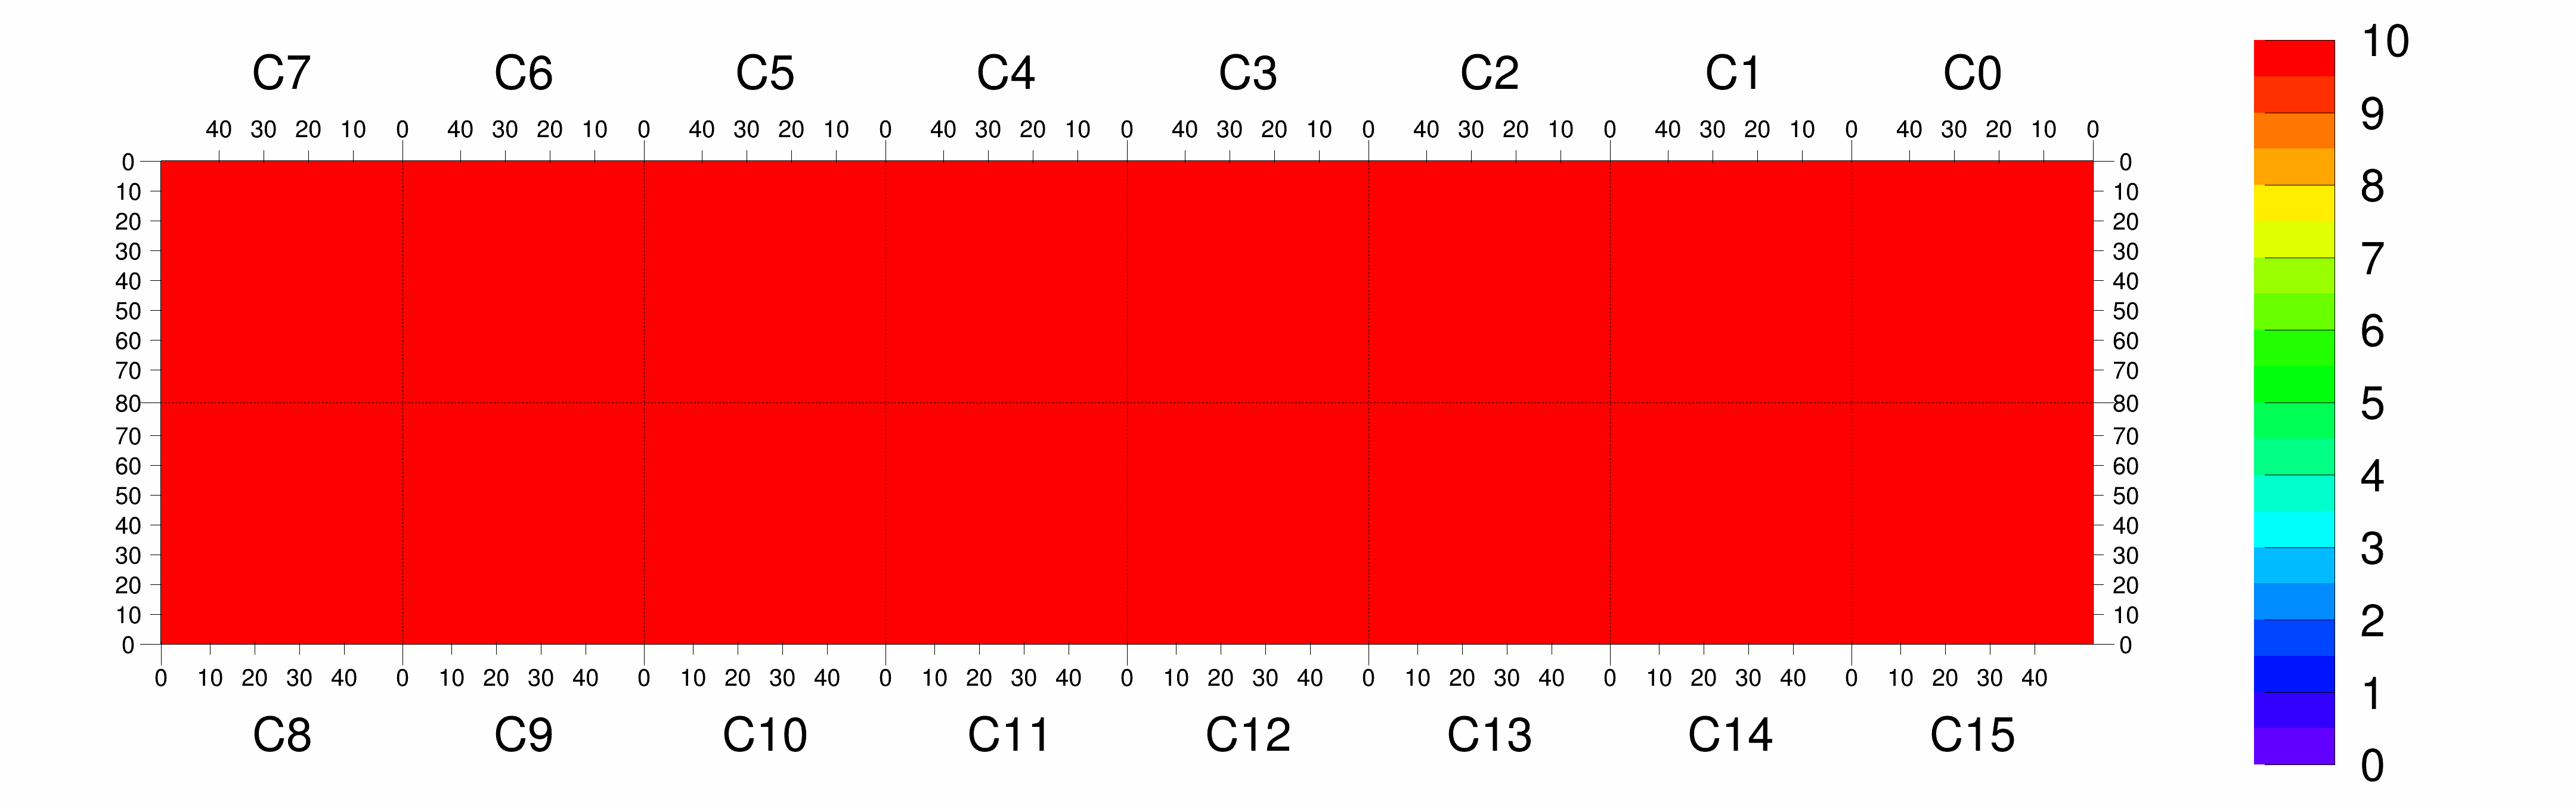
\includegraphics[width=0.3\textwidth]{ch7/pix_ali_good}
   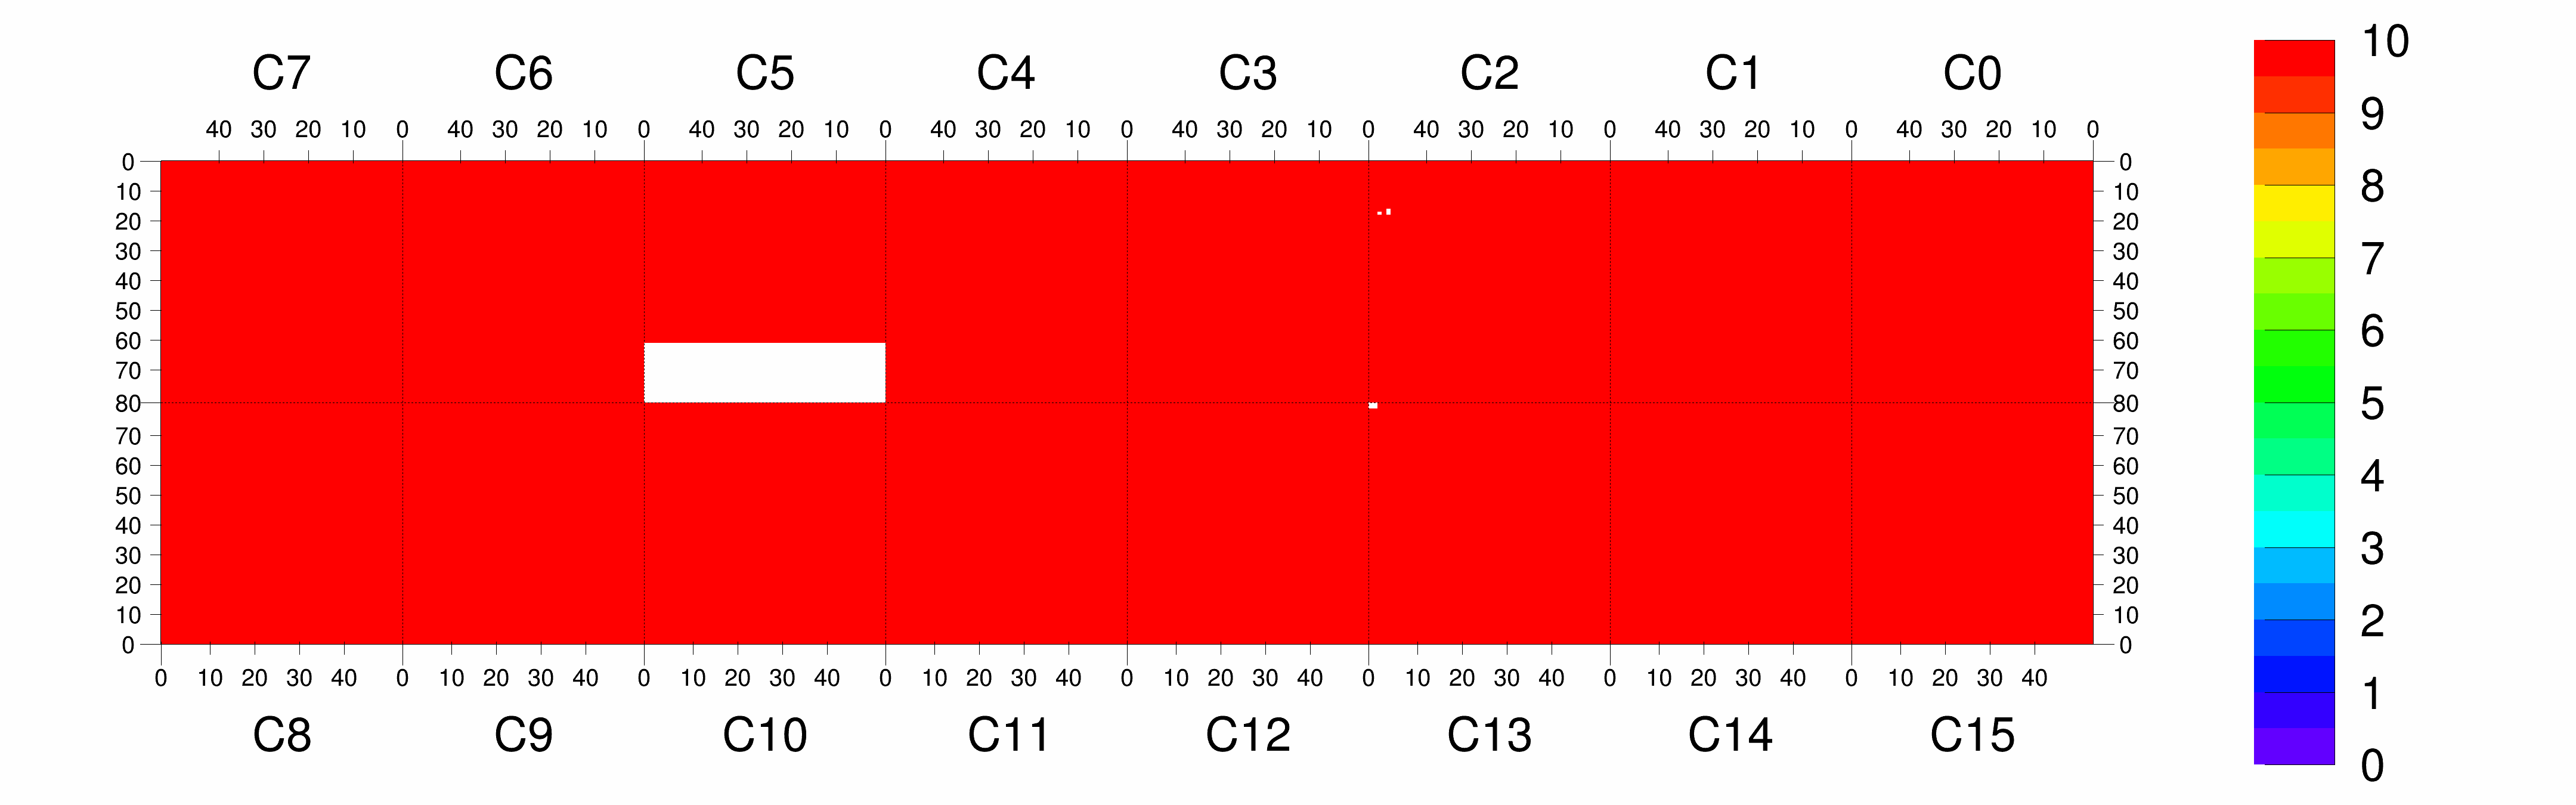
\includegraphics[width=0.3\textwidth]{ch7/pix_ali_bad}
   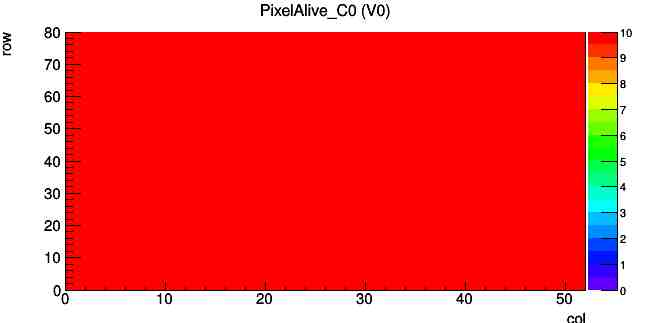
\includegraphics[width=0.3\textwidth]{ch7/pix_ali_full}
  \caption[Pixel alive test]{Pixel alive test for a fully assembled module. a) Alive test, b) Mask test, and c) AddressDecoding test.{\rojo{right fig}}}\label{fig:pix_ali}
\end{figure}

\begin{figure}[!h]
  \centering
   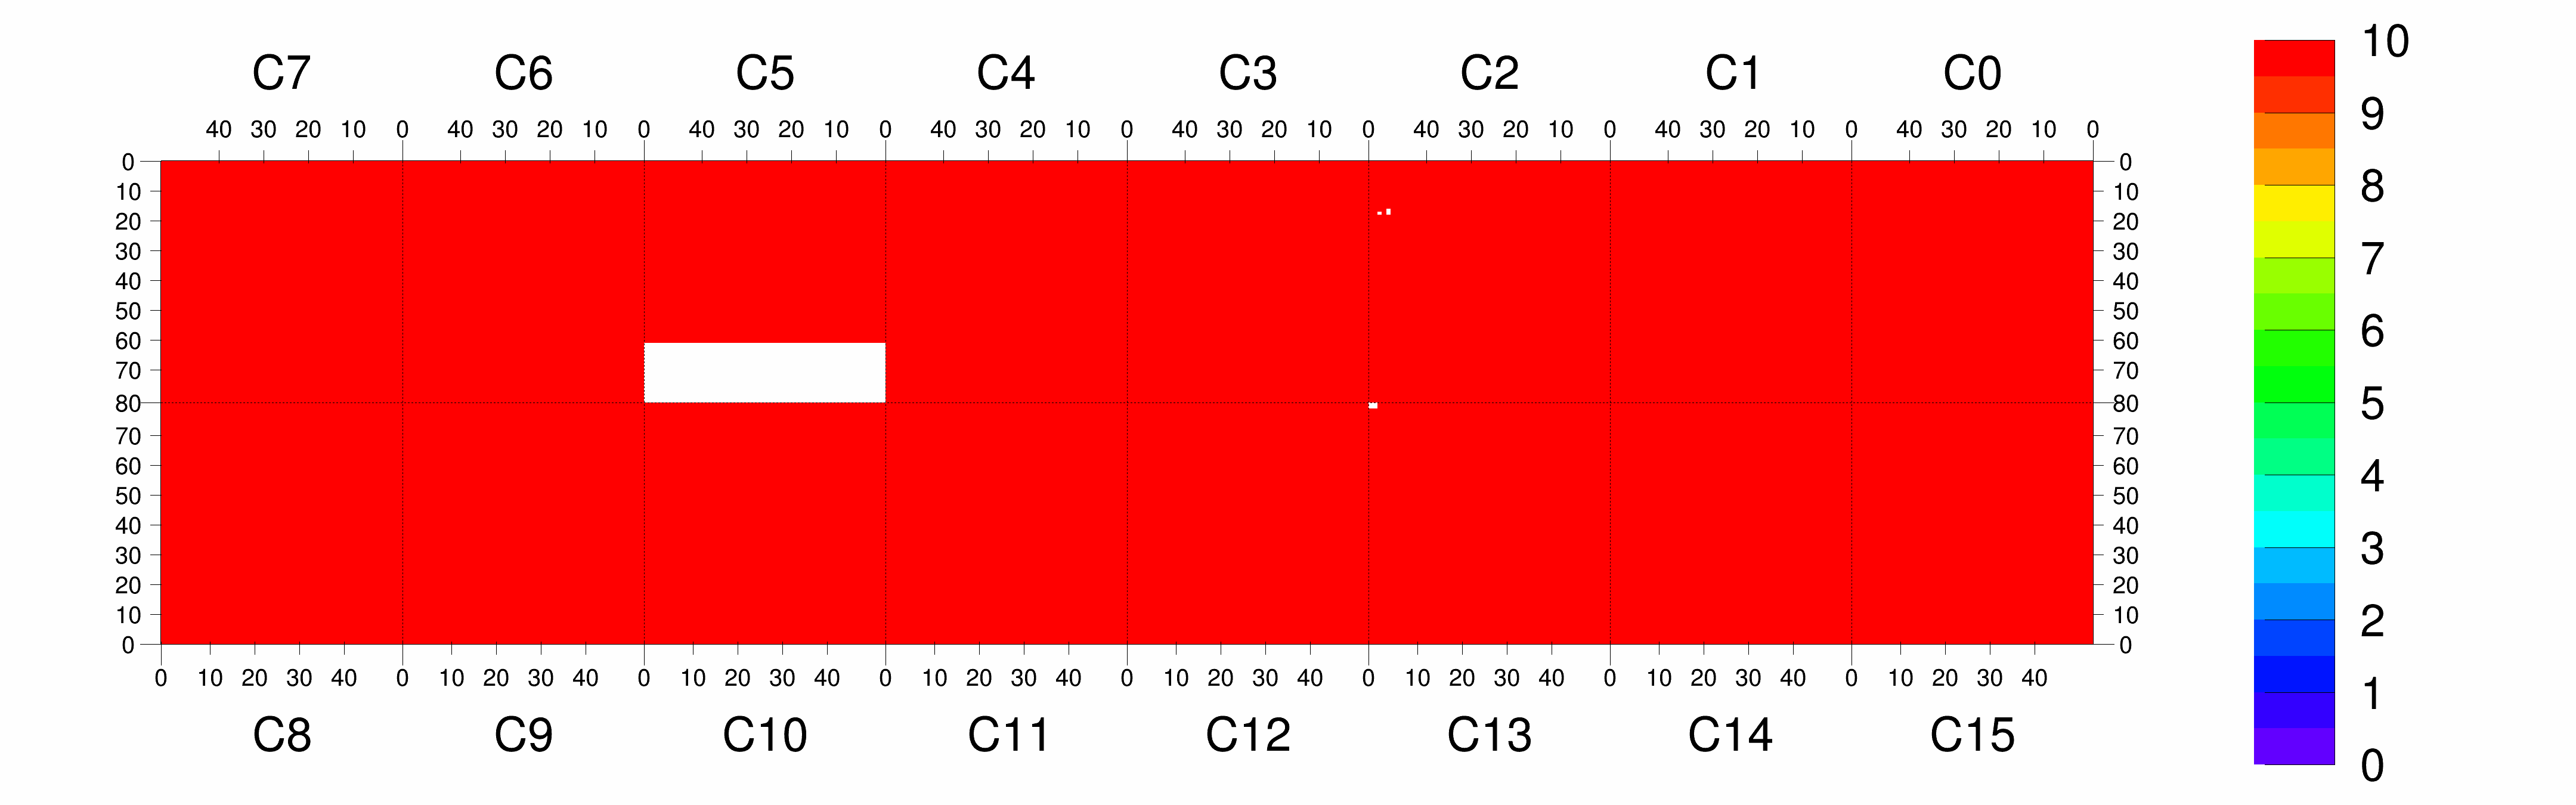
\includegraphics[width=0.4\textwidth]{ch7/pix_ali_bad}
   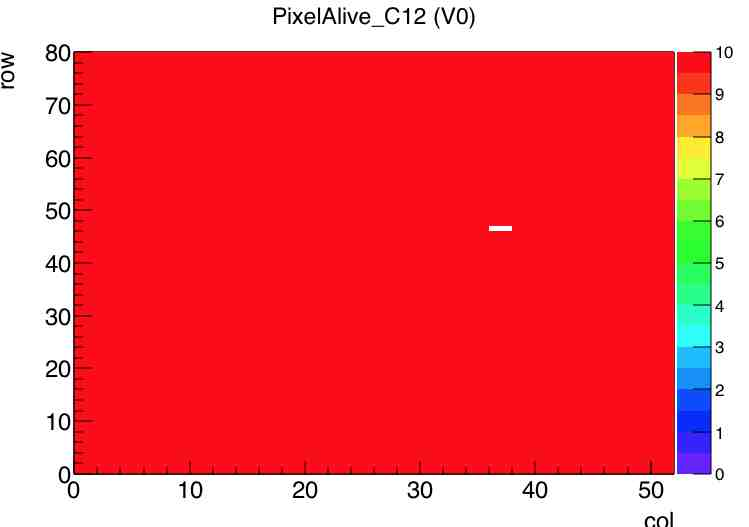
\includegraphics[width=0.3\textwidth]{ch7/pix_ali_roc}
  \caption[Faulty pixel alive test]{Pixel alive for a fully assembled module. a) a module with a faulty ROC and b) a ROC with faulty/dead pixels}\label{fig:pix_ali_bad}
\end{figure}

\subsubsection{Trimming Test}
The aim of the the trimming test is to (calibrate) set the threshold of all pixel on a ROC as uniform as possible. It attempts to do this by varying the VthrComp, Vtrim, and Trim bits DACs. The Trimming test sets VthrComp and Vtrim for the entire ROC and then uses trim bits to further refined the threshold of individual pixels. After the trimming test is finished all pixels within the ROC {\rojo{will have a threshold value as low as possible but still higher than the electrical noise.}}  Furthermore, a TrimBits subtest verifies that all trim bits are working by sequentially enabling each bit and observing its effect on the pixel threshold distribution. The trimming test works as follows: first, with Vcal set to a target value, it finds the VthrComp turn-on value by producing S-Curves for all pixels with respect to VthrComp. Then, VthrComp is set to the value of the pixel with the lowest turn-on value. A ROC map distribution of turn on values for a ROC can be seen in figure \ref{fig:turn-on}. Then, with the VthrComp set to its lowest value, the test tries to minimize the Vtrim value by repeating the previous process and finding the pixel with the highest Vcal turn-on value, see Fig \ref{fig:turn-on}. This is the pixel that requires the most trimming to have its Vcal threshold reduced to the target value. Following, with all trim bits enabled, the test performs an efficiency scan over Vtrim and Vcal DACs \ref{fig:turn-on} to find the value of Vtrim that corresponds to a turn-on at the target Vcal.

\begin{figure}[!h]
  \centering
  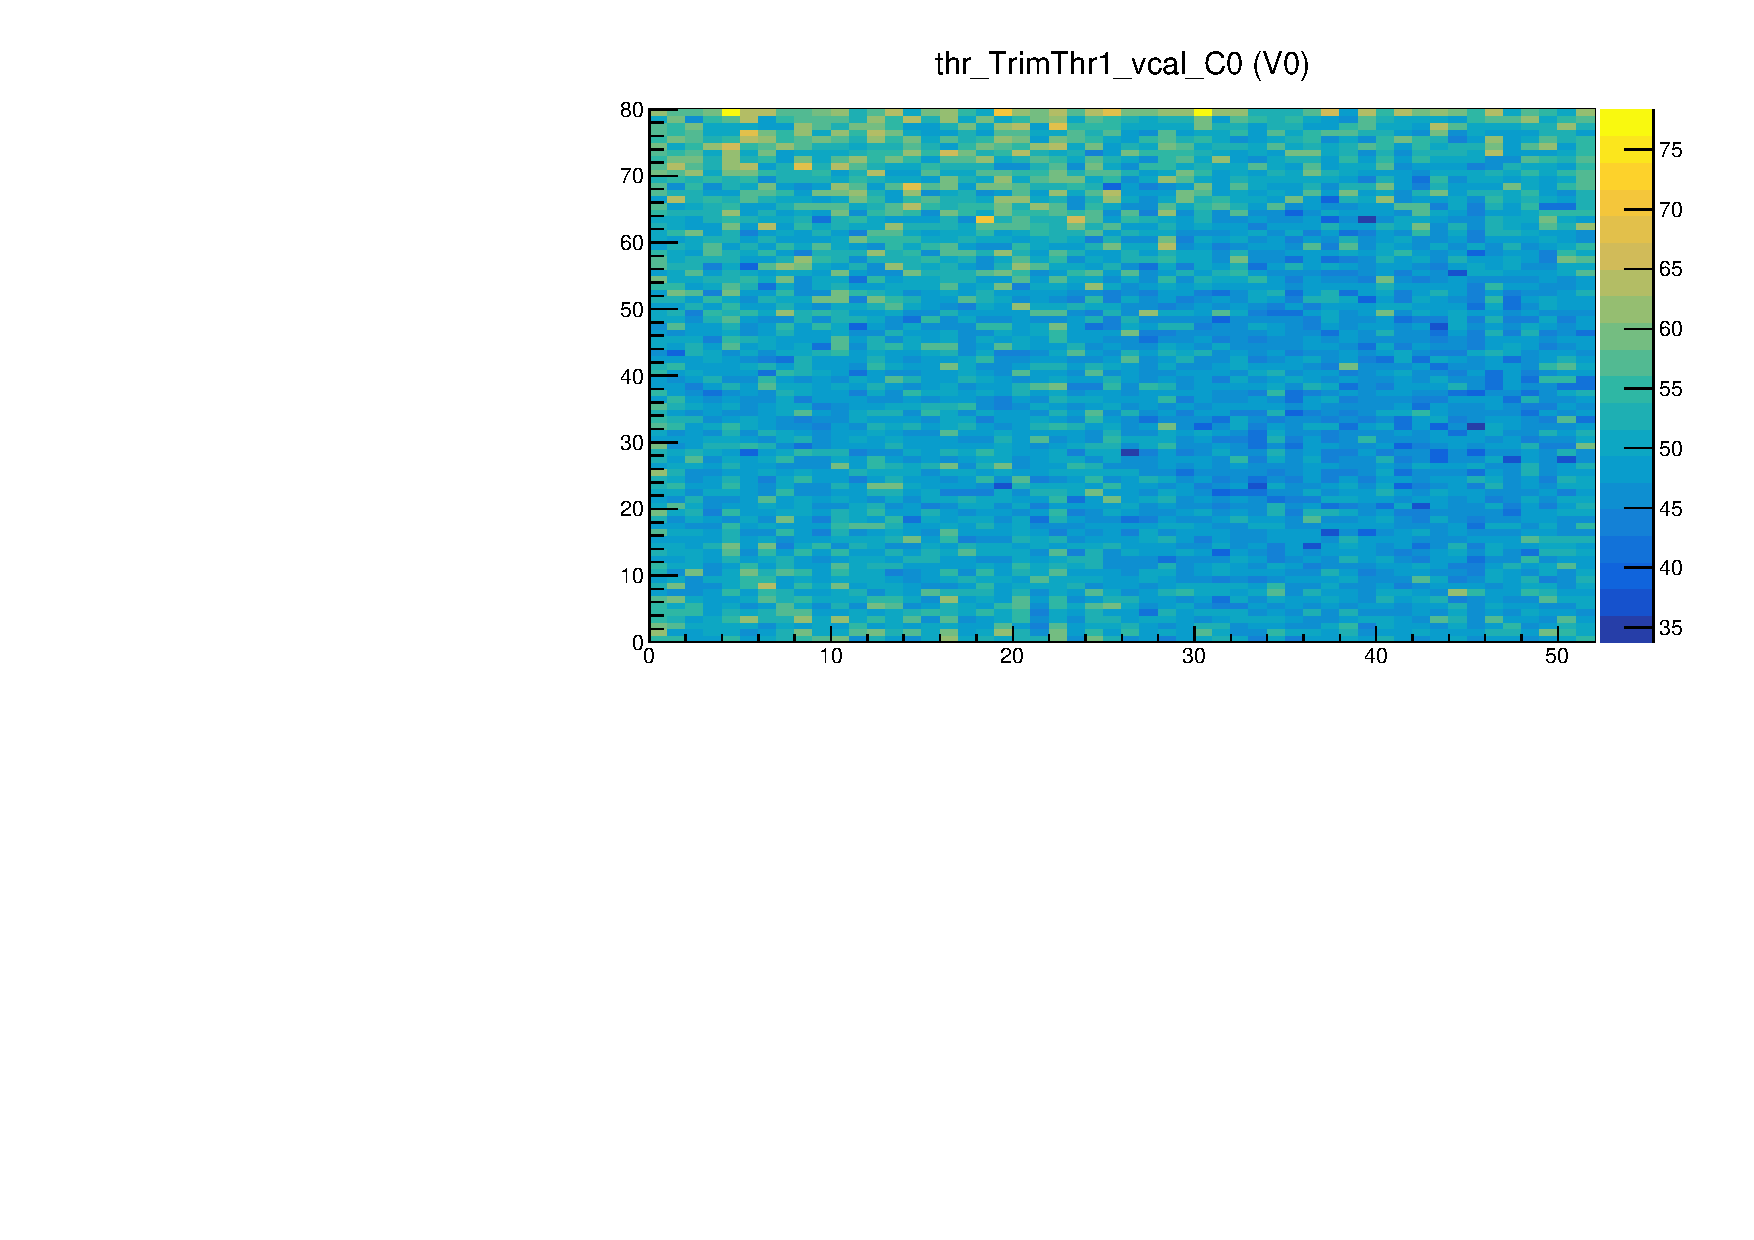
\includegraphics[width=0.3\textwidth]{/ch7/trim_turn-on_vcal}
  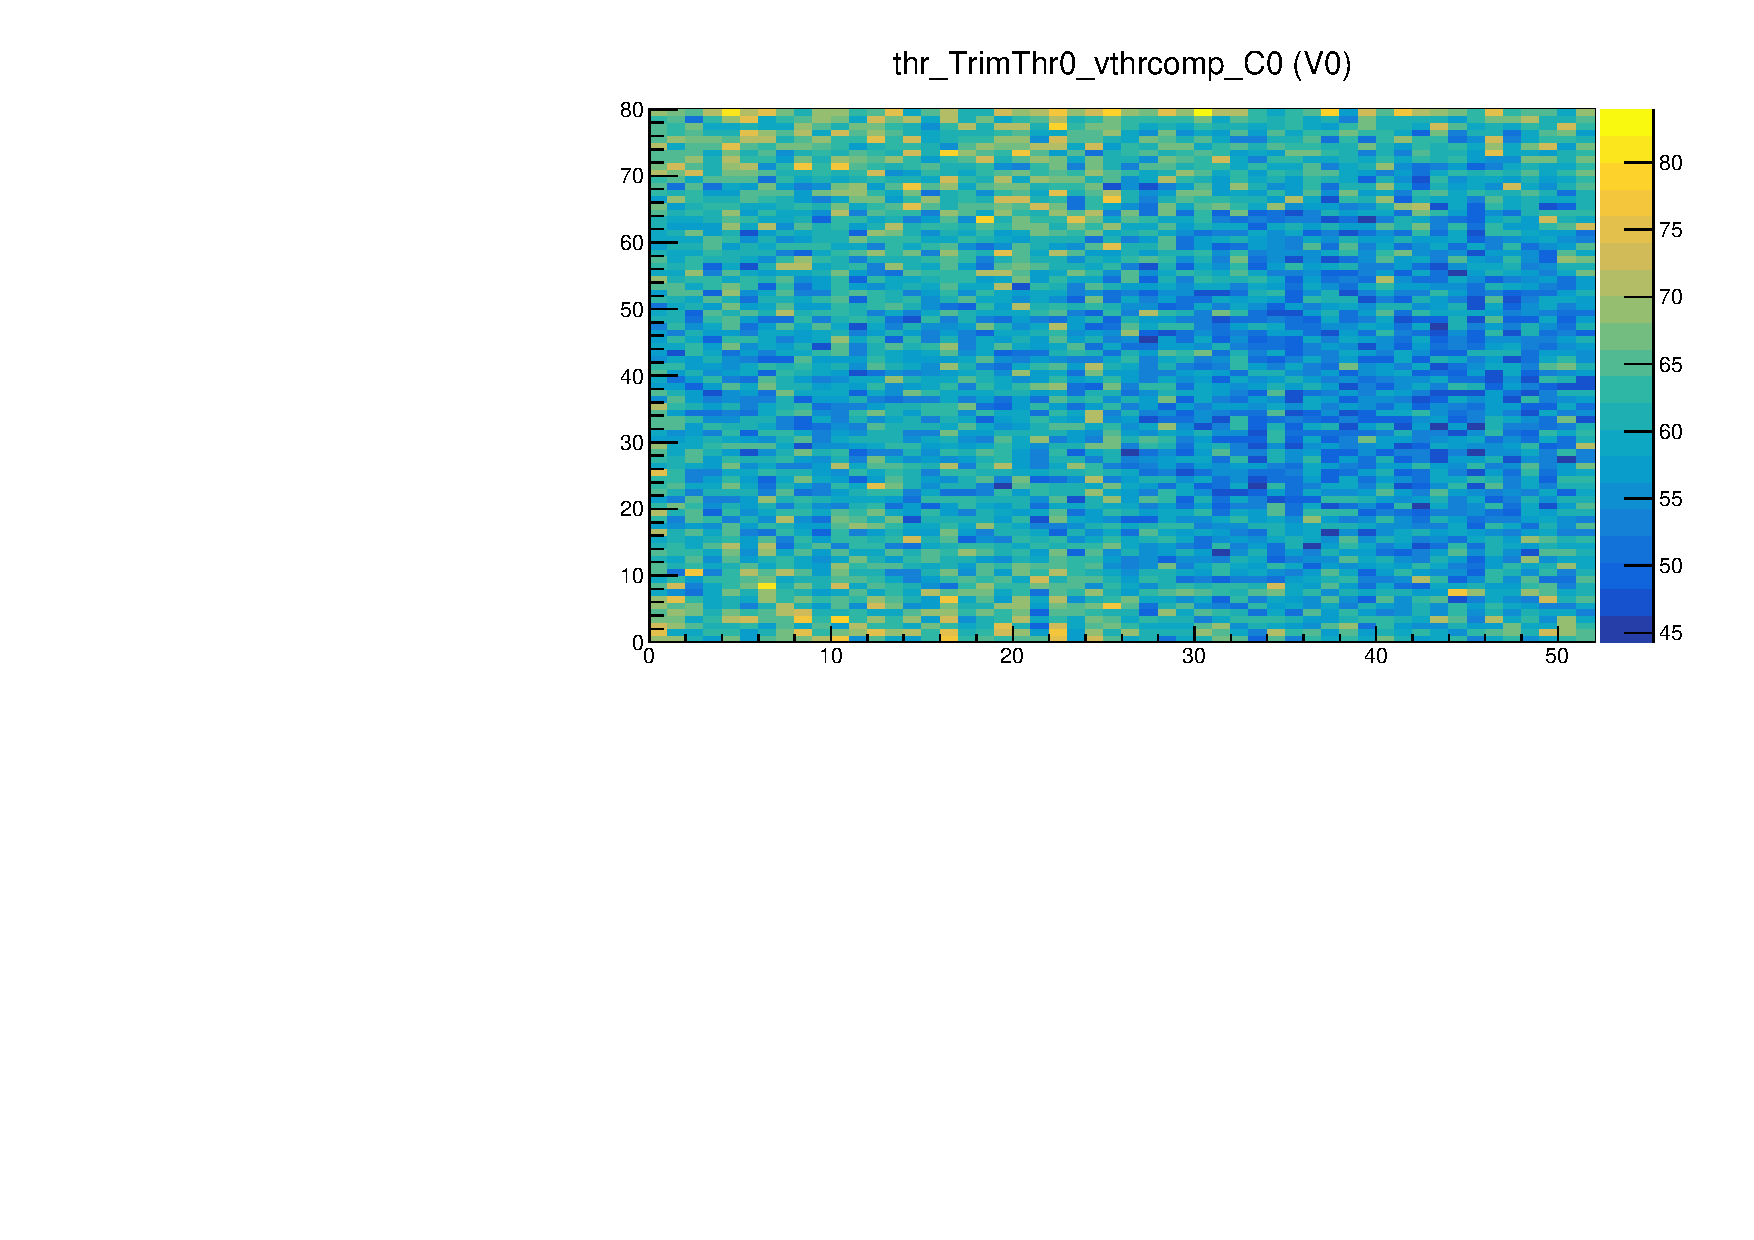
\includegraphics[width=0.4\textwidth]{/ch7/trim_turn-on_vthr}
  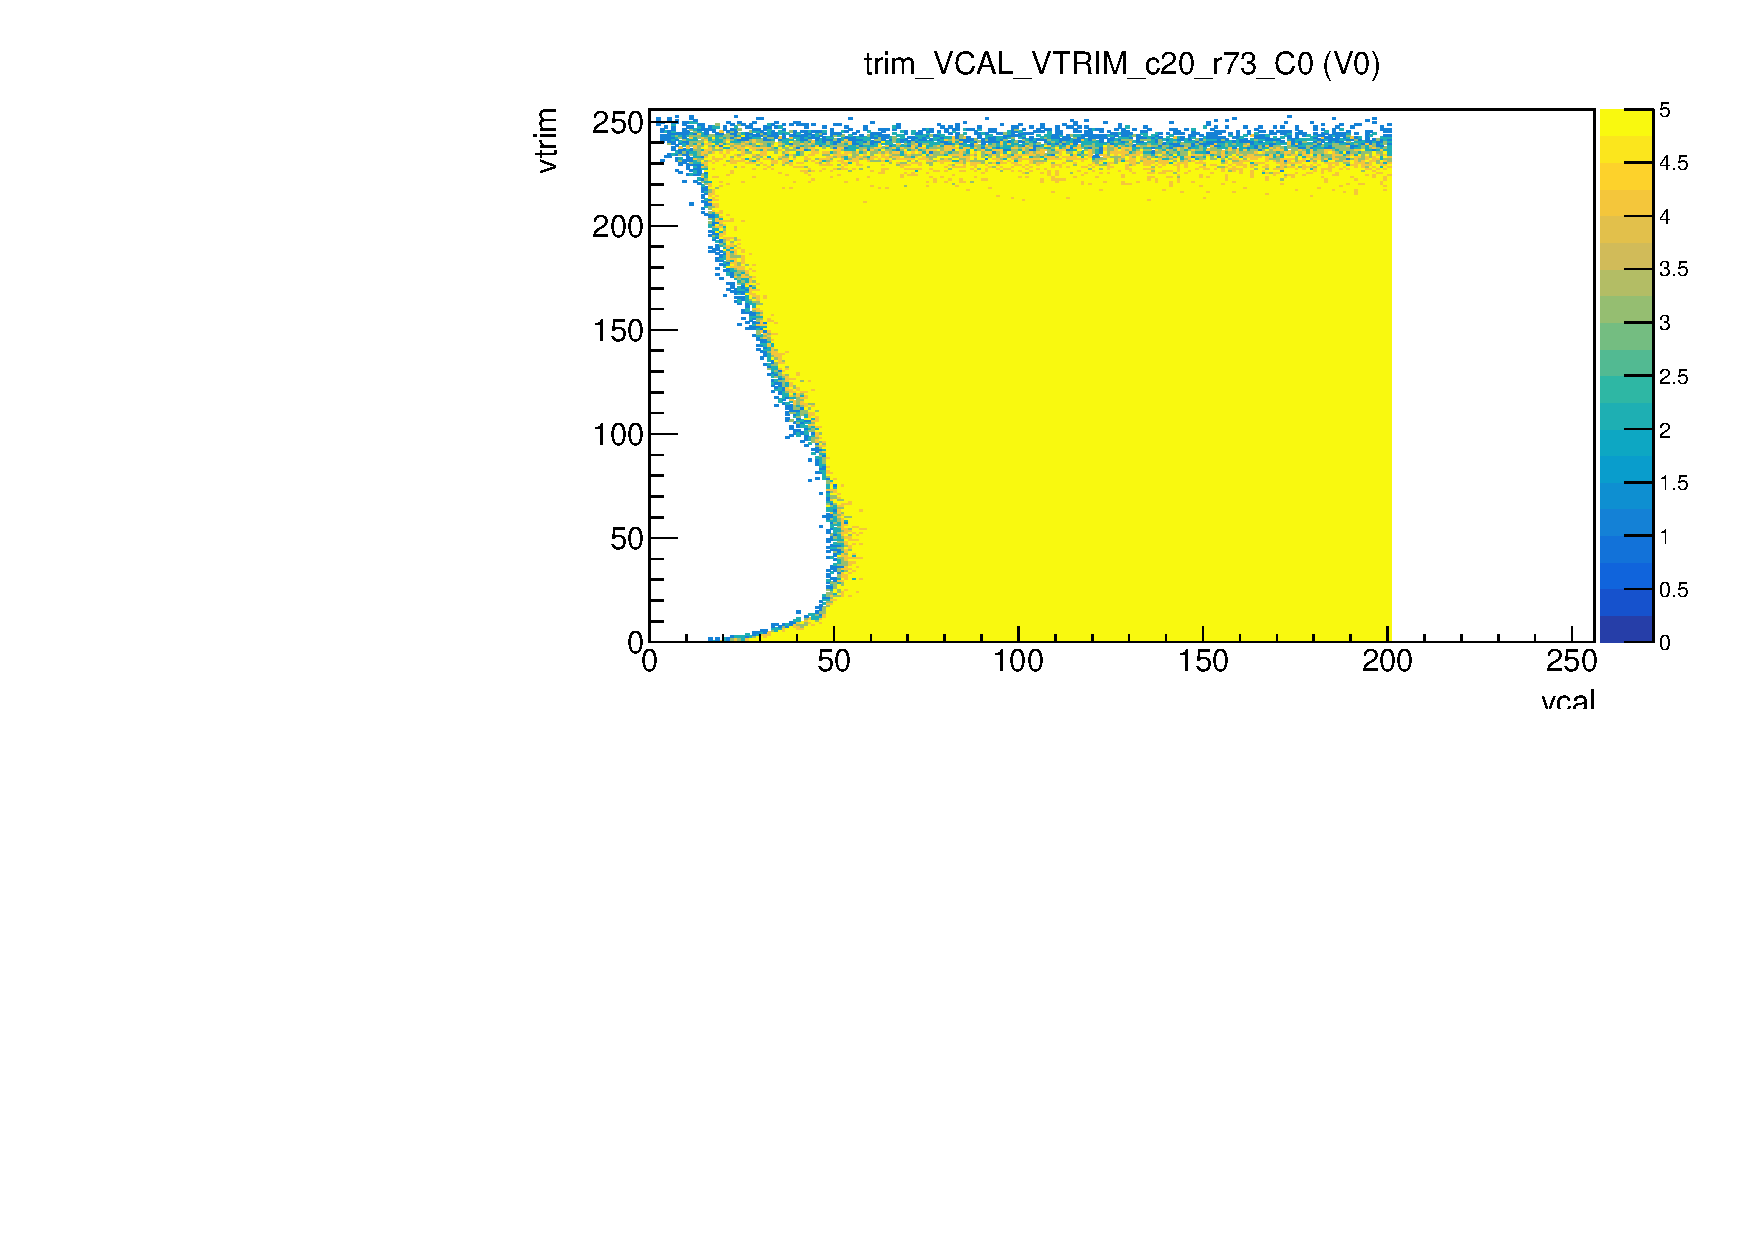
\includegraphics[width=0.3\textwidth]{/ch7/trim_eff}
  \caption[Trim test turn on]{Trim test optimization for. left: Vcal turn on, center: Vthr turn on, right: efficiency in the Vtrim-Vcal plane.}\label{fig:turn-on}
\end{figure}

Next, starting from a high Vtrim, its value is iteratively lowered until the Vcal turn-on surpasses the target Vcal, which corresponds to the minimum value that can trim this pixel. This is the final value of the Vtrim DAC for the the ROC. Finally, with the values of the VthrCaomp and Vtrim set, the test refine the threshold on each pixel by modifying the 4 Trim bits. Starting with the Trim bits set to 7 [0111],    scurves are used to find the Vcal turn-on value. If the pixel {\rojo{reports a hit}} fires below (above) the target Vcal value, the Trim bits value is increased (decreased) by 4, so that the amount of trimming is decreased (increased). This process is repeated three more time increasing or decreasing the Trim bits values by 2, 1, and 1 unit respectively, covering the full range, 0-15, of the Trim bits. Figure \ref{fig:trim_bits} shows a ROC map of Vcal for Trim bits = 7 and after 4 corrections are made and the final Vcal map and distribution could be seen in figure \ref{fig:trim_final}. 

\begin{figure}[!h]
  \centering
  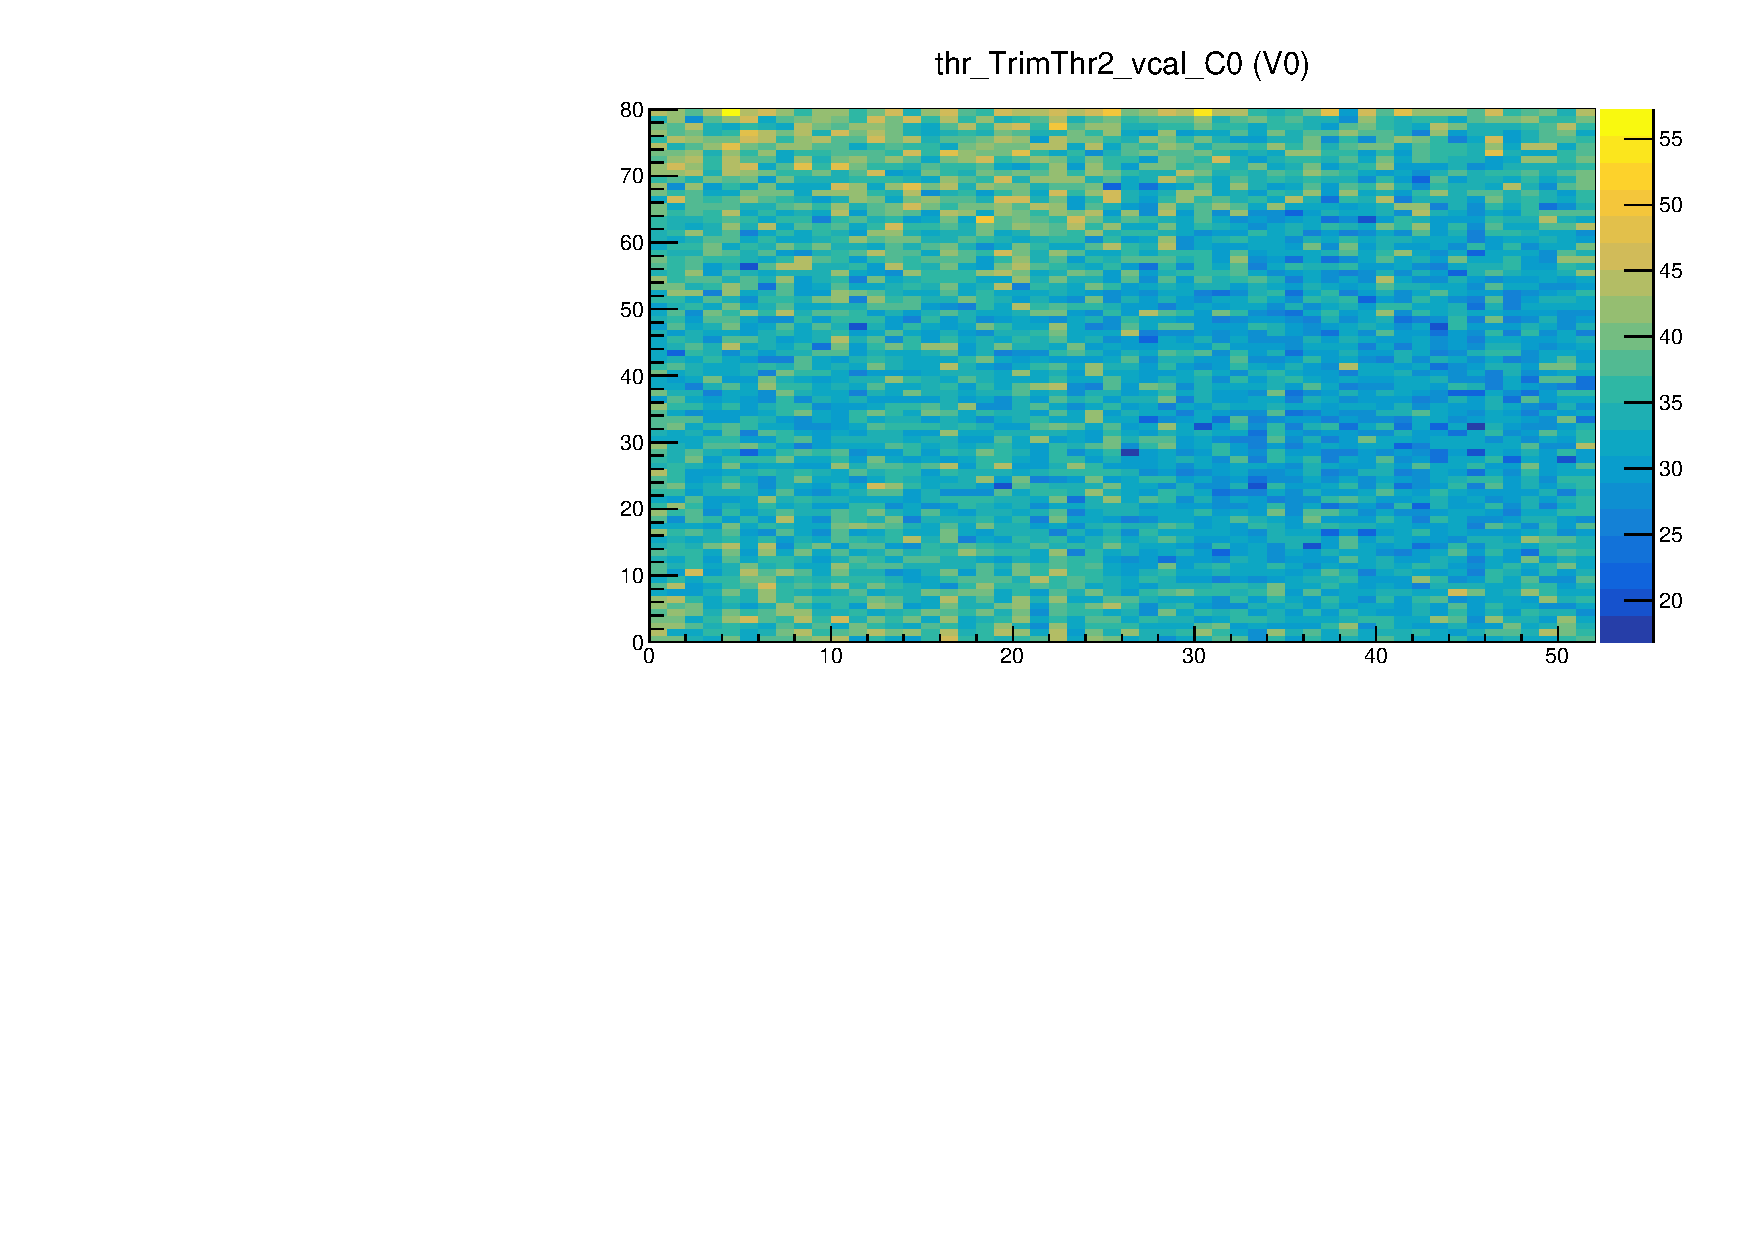
\includegraphics[width=0.7\textwidth]{/ch7/trim_bits_7}
  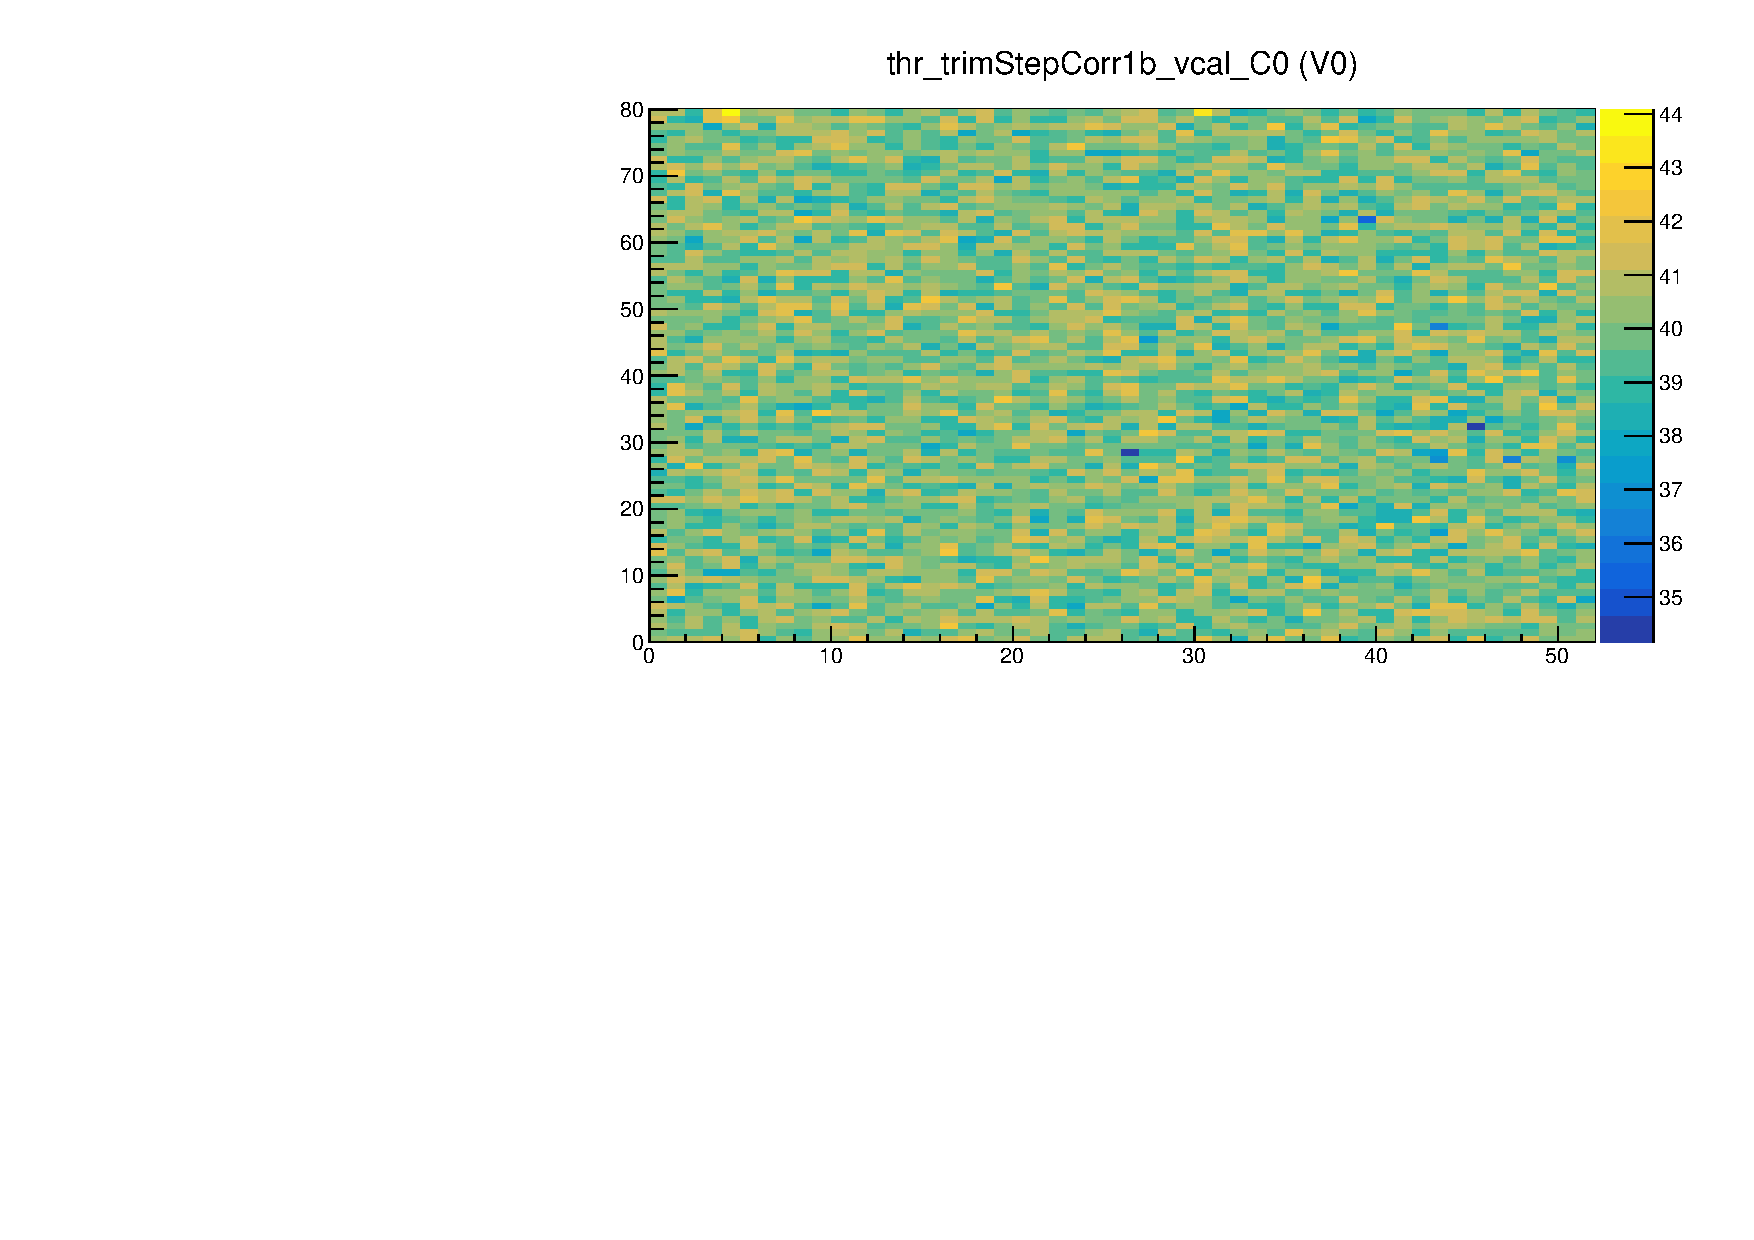
\includegraphics[width=0.7\textwidth]{/ch7/trim_bits_corr}
  \caption[Trim test Trim bits]{Trim bits map distributions for the Vcal turn-on values for the initial  and final Trim bits values.}\label{fig:trim_bits}
\end{figure}

\begin{figure}[!h]
  \centering
  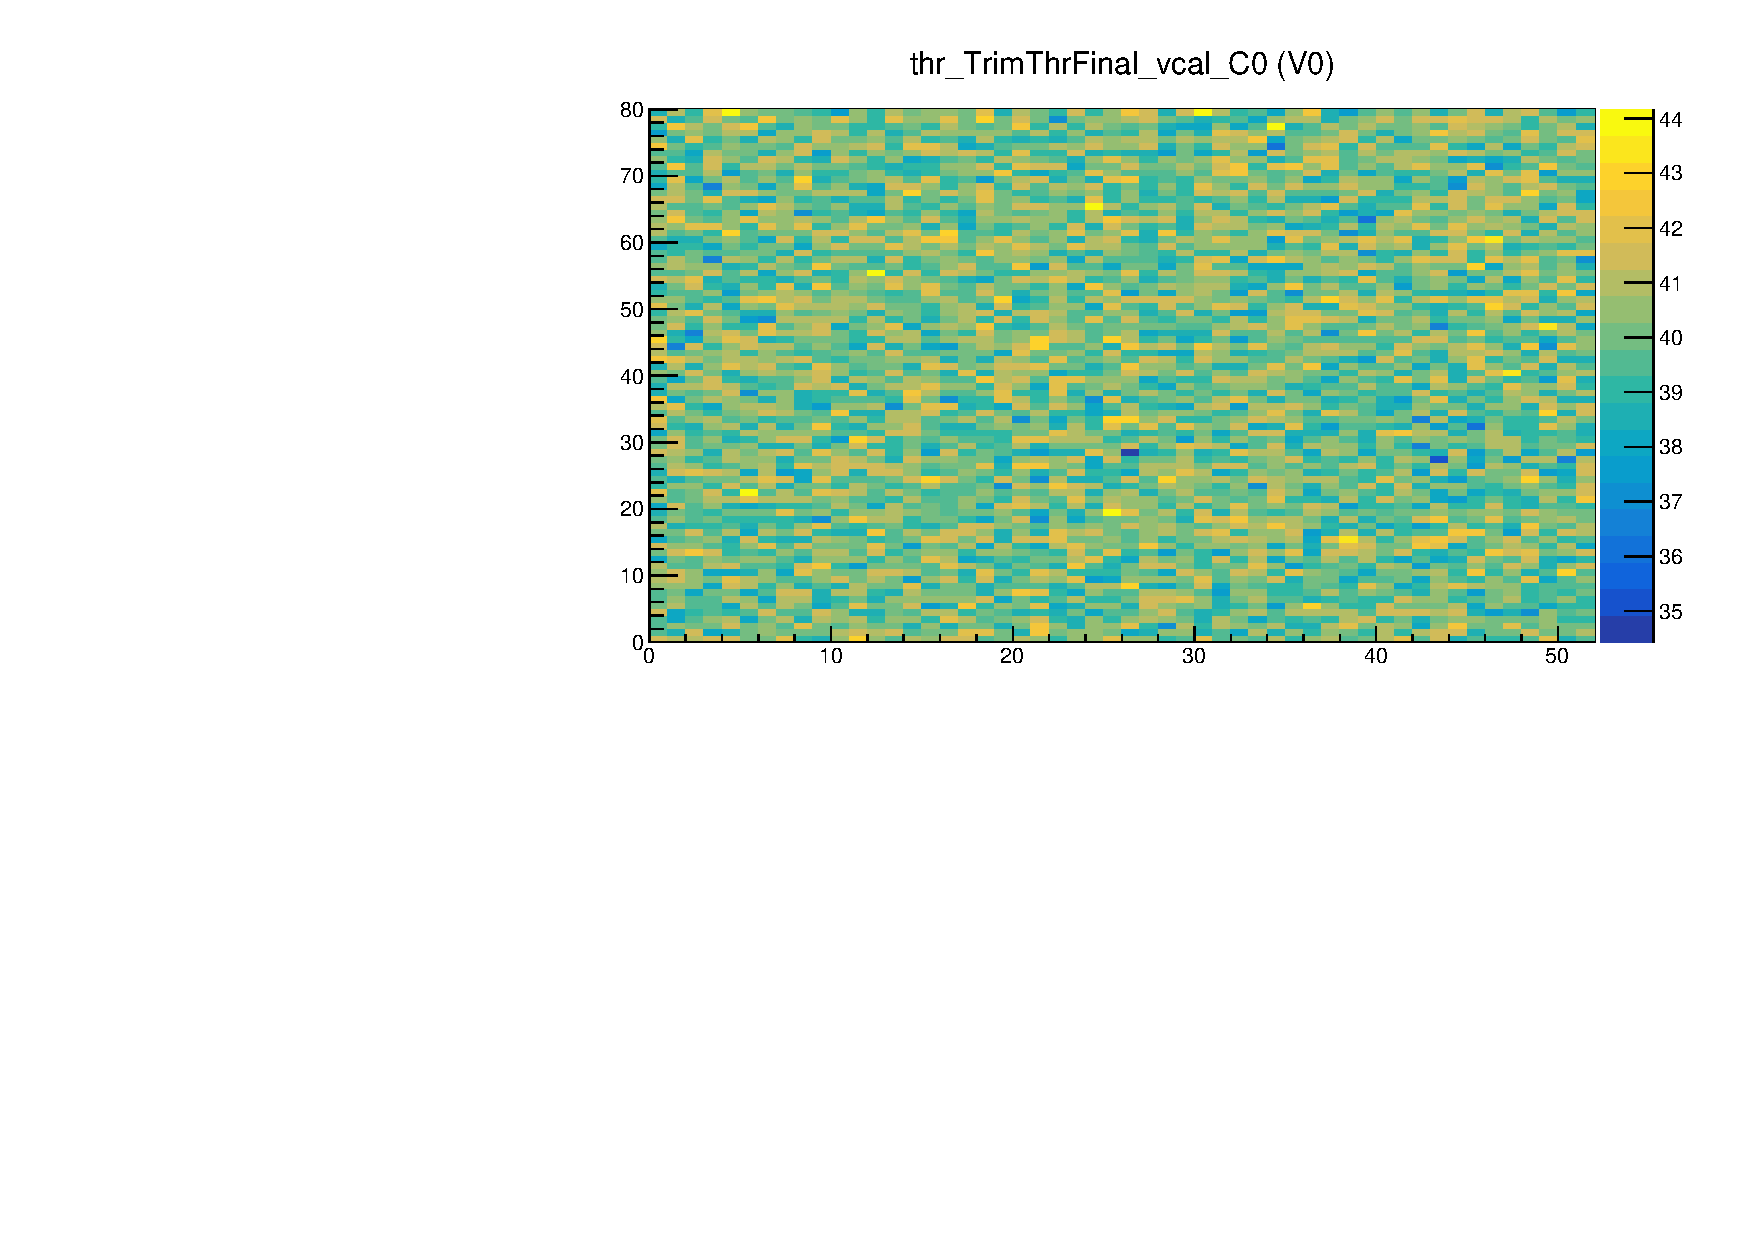
\includegraphics[width=0.7\textwidth]{/ch7/trim_final_map}
  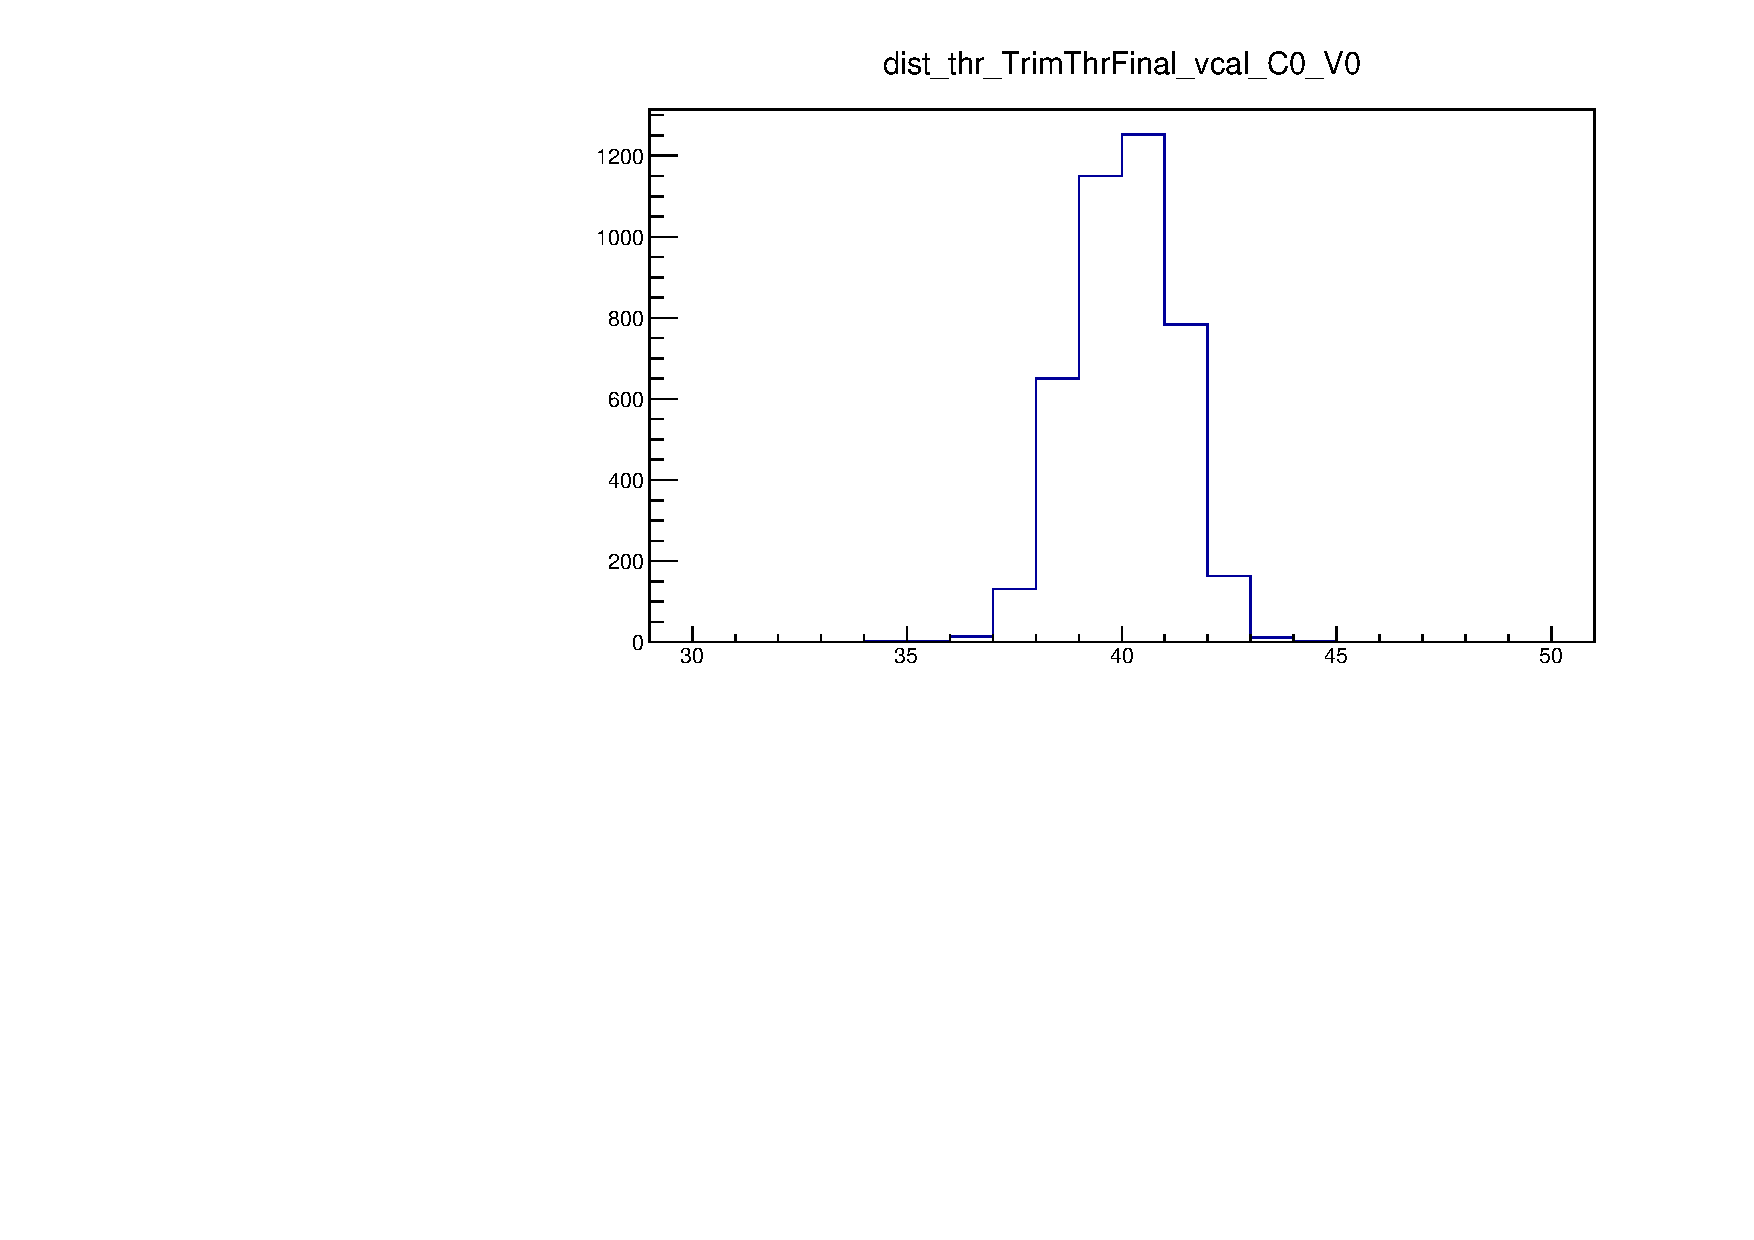
\includegraphics[width=0.7\textwidth]{/ch7/trim_final_dist}
  \caption[Trim test final]{Final map and distribution of Vcal threshold after the Trim test have finished.}\label{fig:trim_final}
\end{figure}

\subsubsection{PH Optimization}
The PHOptimization test is responsible for setting the dynamic range of the output pulse height (PH) as calculated by the ADC serializer. It accomplishes this by optimizing the \ital{PHOffset} and \ital{PHScale} DACs, which adds a constant offset to the pulse height measurement and sets the gain of the ADC. \ital{PHOptimization} works in the following way: First it identifies a low gain and a high gain ensuring it is working (good in pixel alive) and as far as possible from the edges of the sensor. Then, two Vcal signals, low = 60 and high = 255, are sent to each pixel in a ROC and 1D distribution of the PH is created for each vcal value, see figure \ref{phvcal}. A pixel close to the center in each of these distribution is selected as the low and high gain pixel for that ROC.

\begin{figure}[!h]
	\centering
	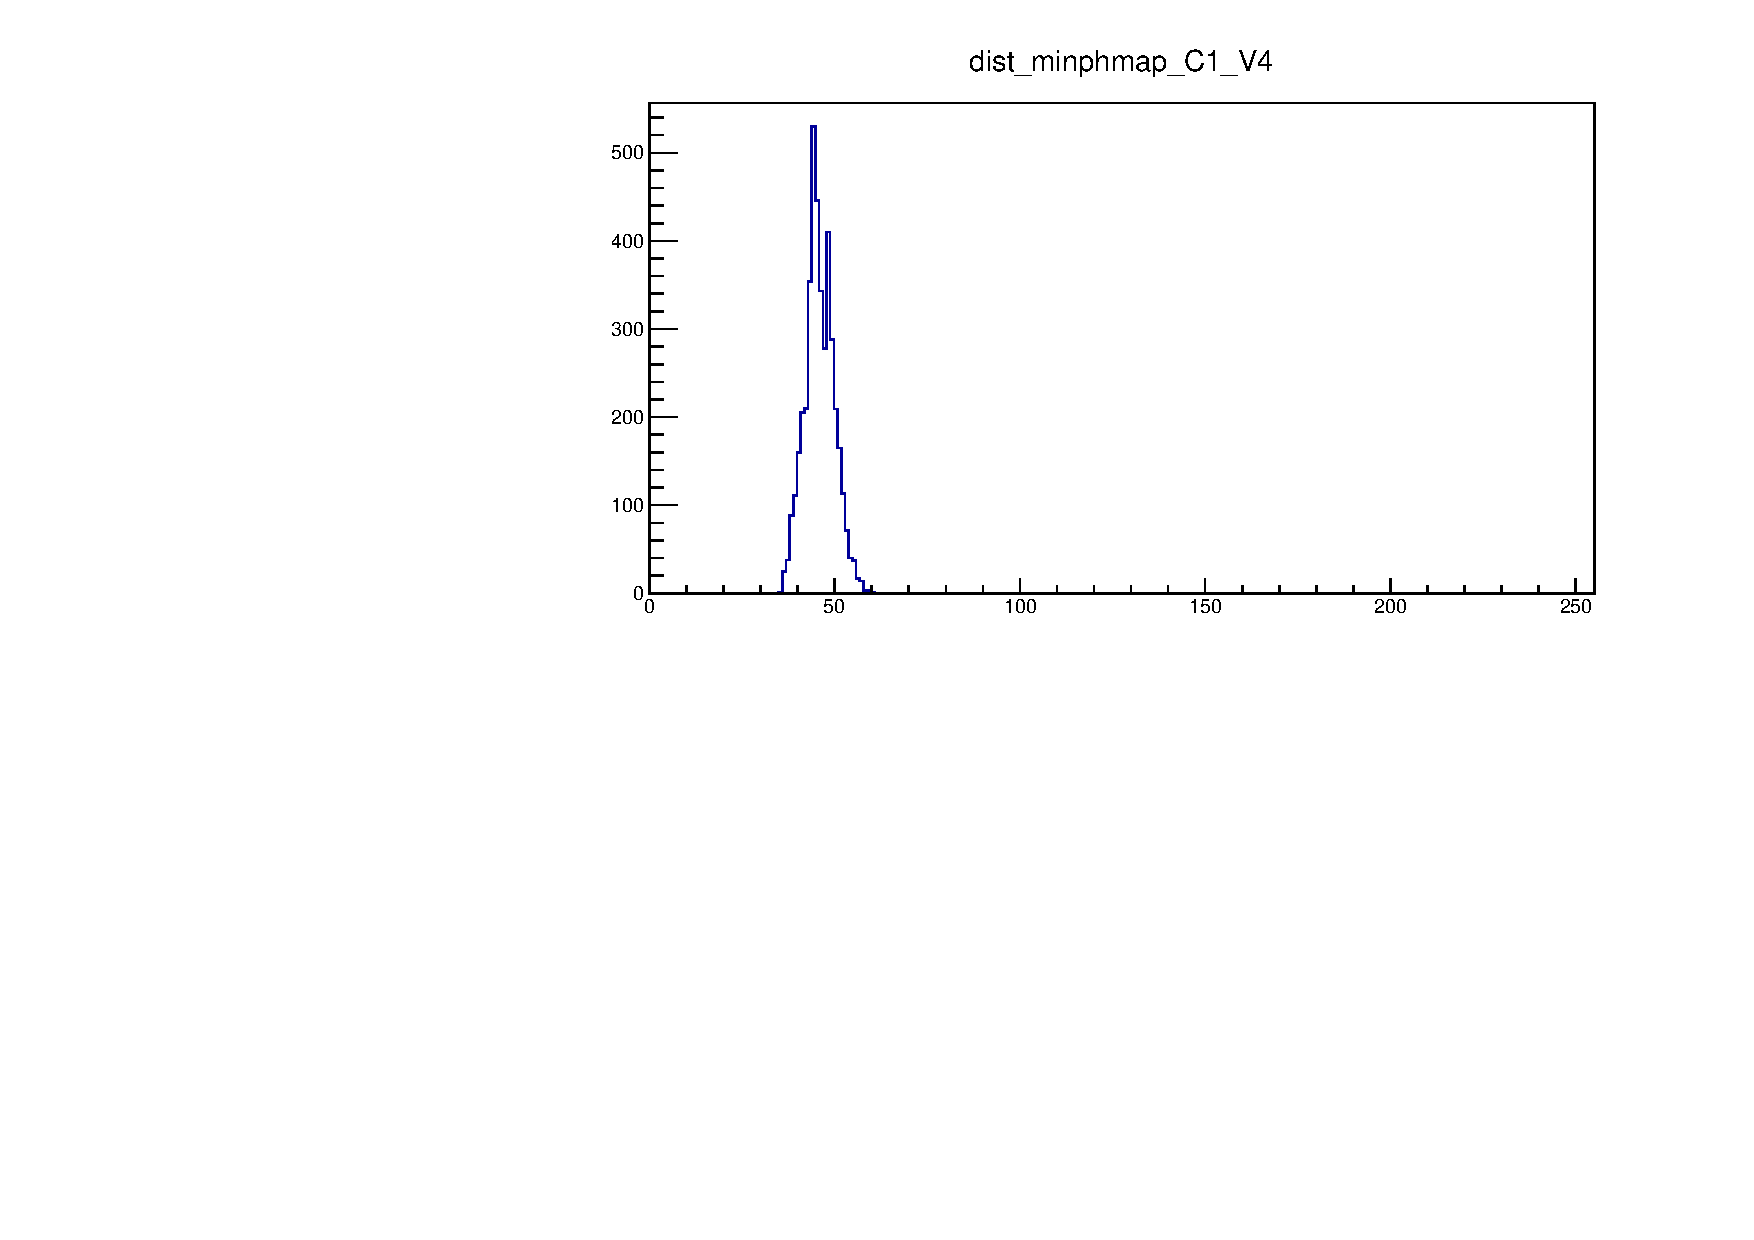
\includegraphics[width=0.5\textwidth]{/ch7/phop_min_dist}
	\includegraphics[width=0.49\textwidth]{/ch7/phop_max_dist}
	\caption[PH vs Vcal]{Distribution of PH as a function of Vcal used to indentify low (top or left) and high (bottom or right) gain pixels.}
	\label{phvcal}
\end{figure}

After both pixels have been identified the test optimizes \ital{PHScale} and \ital{PHOffset} by performing a 2D scan over these two DACs plane. %, using the appropriate Vcal value in each case.
The output of these scan is showing if figure \ref{phovsphs}. The final value of the DACs are chosen from the interception of these two plots as showing in figure \ref{phovsphs}c.  

\begin{figure}[!h]
	\centering
	\includegraphics[width=0.33\textwidth]{/ch7/phop_min}
	\includegraphics[width=0.33\textwidth]{/ch7/phop_max}
	\includegraphics[width=0.32\textwidth]{/ch7/phop_inter}
	\caption[PHOffset and PHScale scan]{Scan on the PHOffset-PHScale plane used to optimize these DACs. a) for a low gain pixel, b) for a high gain pixel, c) interception of a) and b) showing the values of PHOffset and PHScale.}
	\label{phovsphs}
\end{figure}

\subsubsection{Gain Pedestal}
The \ital{Gainpedestal} test measures and records the variation in gain for each pixel in a ROC. Since each pixel will have a different gain these values are needed to calibrate the PH to an input signal. It produces a PH vs. Vcal curvea and fits it with an error function recording the its 4 parameters. Parameter 0 corresponds to
the Vcal value at the center of the error function. Parameter 1 is proportional to the width of the turn-on and is therefore inversely related to the gain of the pixel. Parameter 2 shifts the error function upwards, with a value of unity moving the floor of the function to zero. Parameter 3 corresponds to half the height of the function, and should be near 127.5 (255/2). {\rojo{include equation?}}% y=A*erf(k*(x-x0))+y0
The test also measures the linearity of the pixel response by comparing the integral of the fitted error function in the vcal range to a linear approximation. The results of the test for parameter zero and its linearity are shown in figure \ref{gainped}.

\begin{figure}[!h]
	\centering
	\includegraphics[width=0.6\textwidth]{ch7/gain_ped_p1}
	\includegraphics[width=0.6\textwidth]{ch7/bbbb}
	\caption[Gain pedestal test]{Results of the \ital{GainPedestal} test. a) parameter 0 and b) linearity test {\rojo{find figure}}}
	\label{gainped}
\end{figure}

\subsubsection{Scurve Test}
The SCurve test measures the efficiency of a pixel as a function of Vcal. It is based on the assumption that a pixel will not respond to lower values of Vcal but it will always respond for higher values. In the absence of noise this curve will be just a step function which changes from zero effiecinecy below the threshold to a region of 100\% efficiency above. The effect of the noise is to smear out the step function giving it a \ital{S} shape. As the noise is assume to follow a Gaussian distribution, the SCurve if fitted with an error function and its width is a measure of the noise level in the pixel. Since the Vcal is known at this point in the testing procedure the SCurve is done around this Vcal value. In order to extract an accurate estimate of the width the number of triggers used for the test is 200. The output of this test can seen in figure \ref{fig:scurve}

\begin{figure}[!h]
  \centering
  \includegraphics[width=0.5\textwidth]{ch7/scurve_map}
  \includegraphics[width=0.5\textwidth]{ch7/scurve_dist}
  \caption[Scurve test]{Left: ROC map of the Vcal s-curve turn-on widths. Right: 1D distribution of the vcal scurve width.}\label{fig:vis_insp}
\end{figure}

\subsubsection{Bond Bonding Test}
{\rojo{could be better, include the ROC-Sensor air gap?}} The primary purpose of the \ital{BumpBonding test} is to identify problems with the bumps connecting the sensor to the ROC. The test works by a calibration signal to the sensor via the alternatively path labeled 'sensor calib' \ref{pix_unit_cell}. The signal then reaches the sensor and makes its way to the ROC via the bump bond where it can be normally read. The strength of the signal is measure and compare to the one sent. In the {\ital{pXar} software usually 5 signal of 250 Vcal units are sent to each pixel during a \ital{BumpBonding} test. The {\rojo{output}} of the test is shown if figure \ref{fig:bb_map}    

\begin{figure}[!h]
	\centering
	\includegraphics[width=0.7\textwidth]{ch7/bb_map}
	\caption[Bond bonding test.]{Bond bonding test.}
	\label{fig:bb_map}
\end{figure}

\subsubsection{Summary}
The UNL-HEP module production was a susceesful {\rojo{project}} that culminated with the production and testing of over 500 modules. Figure \ref{mod_ass_time} shows the module production over time for both assembly sites, UNL and Purdue University. Production started slow for the first two months but ramped up after fixing some issues with the parts. Besides that the other time when production almost stopped was around July of 2016 when the BBM provider had difficulties and could not supply BBMs on time. {\rojo{include purdue database}}

\begin{figure}[ht]
	\centering
	\includegraphics[width=0.8\textwidth]{ch7/mod_ass_time}
	\includegraphics[width=0.8\textwidth]{ch7/mod_ass_unl}
	\caption[Module assembly over time.]{Module assembly over time for both assembly sites (top) and for UNL (bottom).}
	\label{mod_ass_time}
\end{figure}

Following the production and testing these of modules a grading scheme was adopted. The grade of a module was given based on the amount of current drawn by it at nominal operating voltages and the number of pixel defects. UNL graded modules at $17$ $^{\circ} C$ but the final grade of the modules was given at FermiLab, where the \ital{Fulltest} was done at $-10$ $^{\circ} C$. Table \ref{tab:mod_grades} shows the grade names and the requirements a module needs to meet to obtain this grade. Since there are 672 modules needed to populate the forward part of the pixel detector and there were not enough grade A modules, some parts of the outer most cylinder was populated with grade B modules.  


\begin{table}
	\centering
	\begin{tabular}{l | c | c | c  }
		Grade & I(V=-150V)  & I(V=-150V)/I(V=-100V)  & Pixel defects\\
		\hline \hline
		A & $<2\mu A$  & $<2$ & $ <1\% $ \\ 
		B & $<10\mu A$ & $<2$  & $ <4\% $ \\
		C & $>10\mu A$ & $>2$ & $ >4\% $  \\    
	\end{tabular}
	\caption[Module grade]{Module grades for the Fpix phase I module production.}
	\label{tab:mod_grades}
\end{table}

Figure \ref{fig:mod_grad_time} shows graded modules over time as well as the module grading by batch received and tested at FermiLab. The integration of the modules into the half cylinders was done at FermiLab, they were later transported to Switzerland and installed into the CMS detector.

\begin{figure}[h]
	\centering
	\includegraphics[width=0.6\textwidth]{ch7/mod_grade_time}
	\includegraphics[width=0.8\textwidth]{ch7/mod_grade_batch}
	\caption[Module grade over time.]{Module grade over time (top) and per received batch at the integration site(bottom).}
	\label{fig:mod_grad_time}
\end{figure}



%\begin{figure}[!h]
 % \centering
 % \includegraphics[width=0.7\textwidth]{../images/ch7/unl_workflow2}
 % \caption[bla for index.]{bla bla.}\label{fig:unl_workflow2}
%\end{figure}
\begin{figure}[!h]
	\centering
	\includegraphics[width=0.7\textwidth]{ch7/thepuc}
	\caption[Pixel unit cell.]{A schematic view of a pixel circuit showing the PUC, CIB, DCP, and some of the relevant DACs.}
	\label{pix_unit_cell}
\end{figure}





